\chapter{L'acoustique}\label{Ch-Acous}
\begin{abstract}
En complément avec ce qui a été vu aux chapitres précédents~\ref{Ch-temps} et~\ref{Ch-ondes} sur les problèmes non stationnaires et les ondes, nous allons nous focaliser dans ce chapitre sur l'acoustique, et plus particulièrement sur le calcul de problèmes pour lesquels les fréquences restent inférieures à quelques milliers de Hz. Nous en profiterons pour effectuer une présentation pratique de l'acoustique et des solutions qui peuvent être mises en œuvre physiquement.
\end{abstract}

Nous avons déjà présenté la problématique de l'acoustique à plusieurs reprises au long de ce document: au paragraphe~\ref{Sec-EqOnde}, l'équation des ondes a été donnée dans le cas de l'acoustique sous forme d'équation différentielle~(\ref{Eq-EqOndeAcou}) dont l'inconnue est la pression acoustique; des remarques plus «physiques» concernant l'acoustique ont été faites au paragraphe~\ref{Sec-EqAcou}, notamment concernant les échelles d'énergies mises en œuvre, ainsi que sur les aspects solidien et aérien; mais c'est surtout au paragraphe~\ref{Sec-EqFblAcou} qu'ont été présentées l'équation d'Helmholtz~(\ref{Eq-Helm})\index[aut]{Helmholtz (Hermann Ludwig Ferdinand von -), 1821-1894, Allemand} et sa formulation faible. Quant à la formulation éléments finis, elle a été abordée au chapitre~\ref{Ch-ondes}, où ont été décrit les systèmes matriciels à traiter selon les cas (réponse libre, périodique ou transitoire, amortie ou non).

Toutefois, nous souhaitions apporter des éléments supplémentaires sur le sujet: 
\begin{itemize}
   \item au paragraphe~\ref{Sec-AcouPhy}, nous proposerons une présentation de l'acoustique «sur le terrain»: nous exposerons brièvement l'acoustique à partir des problématiques qui se posent physiquement, et nous présenterons quelques solutions typiquement utilisées pour résoudre ces problèmes d'acoustique. Nous verrons d'ailleurs que les problèmes rencontrés en hautes fréquences sont généralement aisément résolus, et qu'il convient donc de se concentrer sur les fréquences inférieures à quelques~kHz.
   
   \item au paragraphe suivant~\ref{Sec-AcouMEF} nous reviendrons plus en détails sur la mise en œuvre pratique d'un calcul acoustique par éléments finis.
   
   La motivation principale vient de ce que, dans le paragraphe~\ref{Sec-choc}, nous avons indiqué que la méthode des éléments finis devait se cantonner aux basses fréquences, celles-ci allant jusqu'à 600~Hz environ. Il est vrai qu'au-delà, de nombreuses autres méthodes existent... et nous avions profité de ce paragraphe pour les présenter.
Néanmoins, l'augmentation rapide des capacités des ordinateurs, fait qu'il est tout à fait raisonnable aujourd'hui de traiter des cas allant jusqu'à quelques milliers de Hz, disons 3000~Hz pour fixer les idées, à l'aide de la méthode des éléments finis. Cela permet de traiter la plupart des cas pratiques qui se posent à nous, puisque nous aurons vu auparavant qu'il est souvent inutile de monter plus haut en fréquence.
   
   \item Des illustrations sur quelques cas types seront faites au paragraphe~\ref{Sec-AcouIllus}.
\end{itemize}

\medskip

\medskip
\section{Introduction à l'acoustique physique}\label{Sec-AcouPhy}

Nous nous proposons d'étudier comment une nuisance vibro-acoustique se propage depuis son émission jusqu'à sa réception.
La source pourra être mécanique, aéro- ou hydrodynamique... et pourra couvrir un très large spectre de fréquences, depuis les plus basses (excitation vibratoire, i.e. inférieure à environ 500~Hz), jusqu'aux plus hautes (excitation acoustique, depuis 500 jusqu'à environ 8000~Hz).
La propagation nécessitera de connaître le ou les modes de transmission (solidien, aérien) ainsi que l'environnement de transmission (champ ouvert ou fermé).
La réception quant à elle sera liée à la la perception, qui elle-même sera décrite de manière normative (niveau, puissance) ou sensorielle (psycho-acoustique...).

\medskip
\subsection{Émission}

Face à une problème vibro-acoustique, on est amené à considérer les questions suivantes:
\begin{itemize}
   \item \textcolorblue{Localisation:} où est-ce que ça fait du bruit? Il s'agit de trouver, dans un ensemble qui peut être très complexe (par exemple un véhicule, un compresseur...), où sont les sources.
   \item \textcolorblue{Identification/Séparation:} là où ça fait du bruit, qu’est-ce qui fait du bruit exactement? De manière plus détaillée que la localisation, il peut être nécessaire, pour les sources identifiées, de déterminer la contribution de certaines de leurs parties ou sous-ensembles: selon la modélisation souhaitée, on pourra se contenter de dire que la source vibro-acoustique dans un véhicule est le moteur, où alors souhaiter s'intéresser plus finement aux injecteurs, au carter, à la boîte de vitesse...
   \item \textcolorblue{Enregistrement/Caractérisation:} quel bruit est émis par chaque source? Il s'agit de réaliser des enregistrements permettant de caractériser la source vibro-acoustique considérée. Par exemple, un vibromètre laser permet de récupérer les vibrations (accélérations, vitesses), sans contact. De là, il est possible de re-synthétiser le son d'une seule pièce parmi un ensemble de pièces en fonctionnement. Les enregistrements permettent de caractériser la source en terme de spectre, puissance, directivité... et fournissent également des données utiles pour la restitution de résultats (par exemple données audio binaurales).
\end{itemize}

\medskip
La caractérisation des sources peut également déboucher sur des lois phénoménologiques, qui relient les caractéristiques vibro-acoustiques à certains paramètres tels que par exemple: le rapport de boîte, le régime moteur, le régime ventilateur...
%VM REFS A METTRE

\medskip
Notons enfin que lorsque l'on parle d'acoustique, la propagation finale se fait forcément dans l'air puisque c'est celle qui arrive jusqu'aux oreilles...

\medskip
\subsection{Transmission}

%\medskip
La figure~\ref{Fig-ondes} donne la répartition schématique des puissances (ou les différents types d'ondes à considérer).
\begin{wrapfigure}{l}{65mm}
\centering
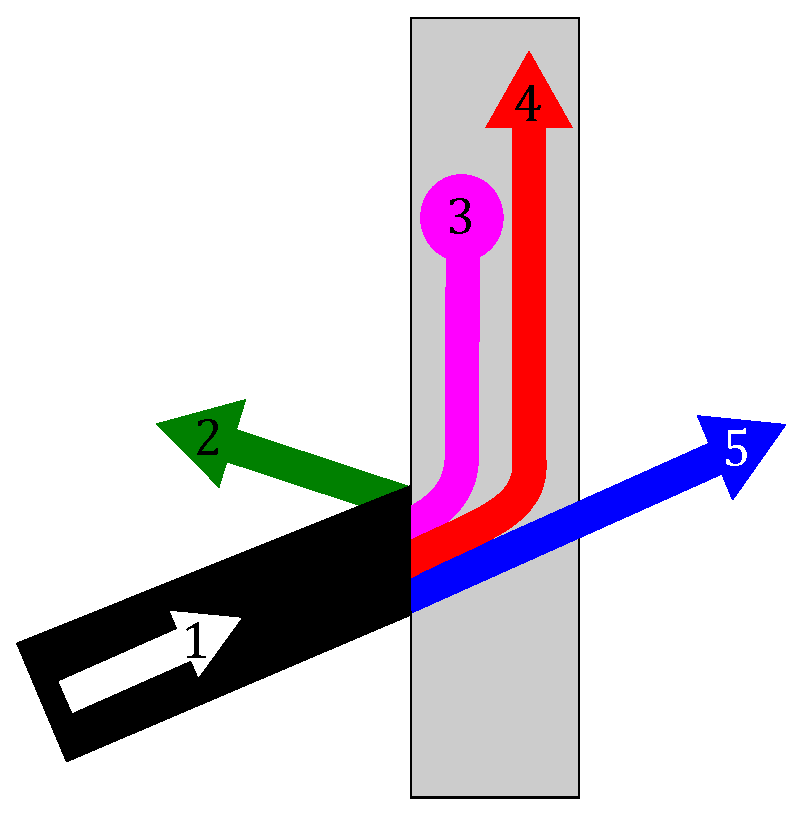
\includegraphics[height=55mm]{ondes.eps}\hspace{1cm}
\caption{Répartition schématique des puissances}\label{Fig-ondes}%: 1 = incidente, \textcolorgreen{2 = réfléchie}, \textcolormagenta{3 = absorbée}, \textcolorred{4 = propagée} et \textcolorblue{5= transmise}}
\end{wrapfigure}
Une onde incidente (1) arrivant sur un obstacle se trouve en partie \textcolorgreen{réfléchie par celui-ci (2)}, alors qu'une partie est directement \textcolorblue{transmise (5)}. Toutefois, cela ne représente pas la totalité de l'énergie incidente, car il reste encore une fraction qui est \textcolormagenta{absorbée ou dissipée par l'obstacle (3)}, et une dernière qui se \textcolorred{propage au sein de l'obstacle (4)} et qui peut ressurgir plus loin dans la structure considérée.

\medskip
Pour les matériaux acoustiques, la réflexion et la transmission seront déduites de mesures en tube d'impédance ou en cabine alpha, la capacité d'isolation sera caractérisée en utilisant la petite cabine, alors que la capacité de rayonnement sera appréhendée par le banc RTC III.

\medskip
L'\textcolorblue{isolement} est une donnée globale qui traduit la capacité d'un ensemble à «faire barrière au bruit». Il s'agit tout simplement de la différence entre ce qui attaque d'un côté et ce que l'on récupère de l'autre. Un isolement donné ne donne donc pas d'information sur la manière dont il est obtenu: réflexion, amortissement, absorption, ou plus probablement par une combinaison plus ou moins complexe (et inconnue) de ces trois phénomènes.

\medskip\ifVersionDuDocEstVincent\newpage\fi
\subsubsection{Modes de propagation}
Comme déjà mentionné au paragraphe~\ref{Sec-EqAcou}, il peut être nécessaire de considérer un ou plusieurs des modes de propagation suivants:
\begin{itemize}
\item \textcolorblue{solidien/solidien:} la source excite mécaniquement la structure, et la vibration se propage dans la structure;
  \item \textcolorblue{aérien/aérien:} la source émet une vibration (un bruit) qui se propage dans l'air (en général). il s'agit de la propagation d'une onde acoustique de sa source jusqu'au récepteur, dans l'air;
  \item \textcolorblue{solidien/aérien:} il s'agit du cas du rayonnement. La source excite  mécaniquement une structure, et celle-ci ré-émet une onde dans l'air. 
  \item \textcolorblue{aérien/solidien:} dans le cas de sources acoustiques très puissantes, l'excitation acoustique se propageant dans l'air peut arriver à faire vibrer une structure.
\end{itemize}
Dans les deux premiers cas, on doit résoudre un problème de propagation dans un milieu (structure ou air). La sollicitation dépend du temps, donc on peut appliquer ce qui a été vu au chapitre~\ref{Ch-temps}; mais comme elle est généralement périodique, et que l'on s'intéresse au régime stationnaire, on peut alors utiliser ce qui a été vu au chapitre~\ref{Ch-ondes} sur les ondes.

Dans les deux derniers cas, il s'agit d'un calcul où il faut prendre en compte le couplage fluide-structure. La source étant périodique, on utilise encore ce qui a été vu au chapitre~\ref{Ch-ondes}, aussi bien dans la structure que dans l'air. Évidemment, ce sont les techniques du chapitre~\ref{Ch-temps} qui s'appliquent si l'on s'intéresse au régime transitoire.

\medskip
Dans la «réalité», tous ces cas existent bien:
\begin{itemize}
  \item solidien/solidien: tout moteur, même monté sur des silenblocs qui filtrent l'excitation, génère dans les supports, puis dans toute la structure porteuse, des vibrations. On est donc bien face à la propagation de vibrations au sein de solides;
  \item aérien/aérien: si l'on n'entre pas dans le détail de son fonctionnement mécanique, un haut-parleur est une source aérienne qui génère une onde acoustique qui se propage dans un volume d'air contenu, par exemple, dans une salle. Si l'on s'intéresse au niveau de pression acoustique en un point de la salle, on a une modélisation où seul le volume intérieur de la salle est nécessaire (et les bonnes conditions aux limites, mais nous y reviendrons);
    \item solidien/aérien: dans le cas de structures en treillis portant des panneaux, ce qui est le cas pour la conception de cars et bus, le moteur, situé à l'arrière, excite la structure de manière solidienne... et des vibrations se propagent dans tout le bus, où elles trouvent régulièrement, et jusqu'à l'avant, des panneaux qui vont se mettre à rayonner, i.e. à transformer cette vibration mécanique en bruit se propageant dans l'air jusqu'aux oreilles du conducteur et des passagers;
  \item aérien/solidien: dans le cas de structures légères, par exemple pour des véhicules sans permis, le moteur excite la structure non seulement de manière solidienne, mais également de manière aérienne. Le bruit généré par le moteur est tel, au sein du compartiment moteur, que cette sollicitation aérienne est capable de faire vibrer le tablier de séparation moteur/habitacle, qui dans ce cas précis est généralement très peu isolant (typiquement en ABS thermoformé avec une épaisseur avant transformation d'environ 3~mm, donc une épaisseur, dans les endroits les plus déformés, de l'ordre du millimètre). Il suffit pour le mettre en évidence de remplacer le moteur par un haut parleur découplé du châssis et générant une pression acoustique équivalente à celle du moteur.  
\end{itemize}
Tous ces cas existent donc bien, et peuvent même se superposer. Il convient donc d'être prudent dans le choix de la modélisation la plus adaptée au problème étudié.

\medskip
%\subsubsection{Les trois «lois» de l'acoustique}
\subsubsection{Fonctionnement des solutions acoustiques}

Il en va de même dans l'utilisation de matériaux ou solutions acoustiques. Plusieurs phénomènes peuvent intervenir et se superposer:
\begin{itemize}
   \item \textcolorblue{absorption:} il s'agit du cas où l'énergie acoustique est dissipée dans ou par le matériau ou la solution. Pour les matériaux poreux ou fibreux, des modèles de fluides équivalent existent. Ils sont modélisés par des paramètres tels que la porosité, la tortuosité... dans le cas de résonateurs ou de foils absorbers, ce sont les caractéristiques du matériau constituant ceux-ci ainsi que leur géométrie qui déterminent leur performance d'absorption;
   \item \textcolorblue{isolation:} il s'agit du cas où l'on fait barrière au bruit. Les notions d'étanchéité et de masses sont prépondérantes. On commencera donc par éviter au maximum toutes les fuites acoustiques (tous les trous). Ensuite, on pourra utiliser le fait que l'isolation est liée à la masse: on gagne 6~dB par doublement de masse (en fait $20\log_{10}2$).

Enfin, d'autres systèmes peuvent être utilisés. Parmi ceux-ci, le système «masse-ressort» constitue l'une des plus anciennes solutions pour améliorer l'isolation acoustique. Il s'agit de réaliser un système rudimentaire de double parois découplées. Lorsque la première paroi est attaquée par le bruit et les vibrations, la seconde réagit de manière découplée. On peut choisir le ressort et la masse pour «filtrer» les fréquences indésirables. Ce système présente par contre une fréquence de coupure pour laquelle l'isolation n'est pas améliorée, mais au contraire le phénomène est amplifié.
   
   \item \textcolorblue{amortissement:} il s'agit du cas où l'énergie vibratoire est dissipée dans un matériau choisi pour ses propriétés d'amortissement visqueux, ou par son mode de fixation (collage, montage en contrainte...).
\end{itemize}
L'ajout d'une pièces d'insonorisation, par exemple réalisée par thermocompression de matières fibreuses, sur une structure a pour effet d'augmenter l'absorption. Toutefois, cette pièce possède une masse, même faible, qui ajoute de l'isolation. De plus, son mode de fixation peut apporter de l'amortissement à la structure étudiée. Toutefois, si la pièce est montée sur une tôle, sa masse étant vraiment faible face à celle de la tôle, il n'est pas faux de ne pas prendre en compte son apport sur l'isolation. Si de plus elle est juste maintenue mécaniquement, il est également possible de négliger son influence en terme d'amortissement.

\medskip
\subsubsection{Compléments sur l'absorption}

Revenons quelques instants sur l'\textcolorblue{absorption}, et plus particulièrement sur les performances d'absorption des solutions existantes, qui sont illustrées sur la figure~\ref{Fig-mtxalpha}.
\begin{figure}[h!]
\centering
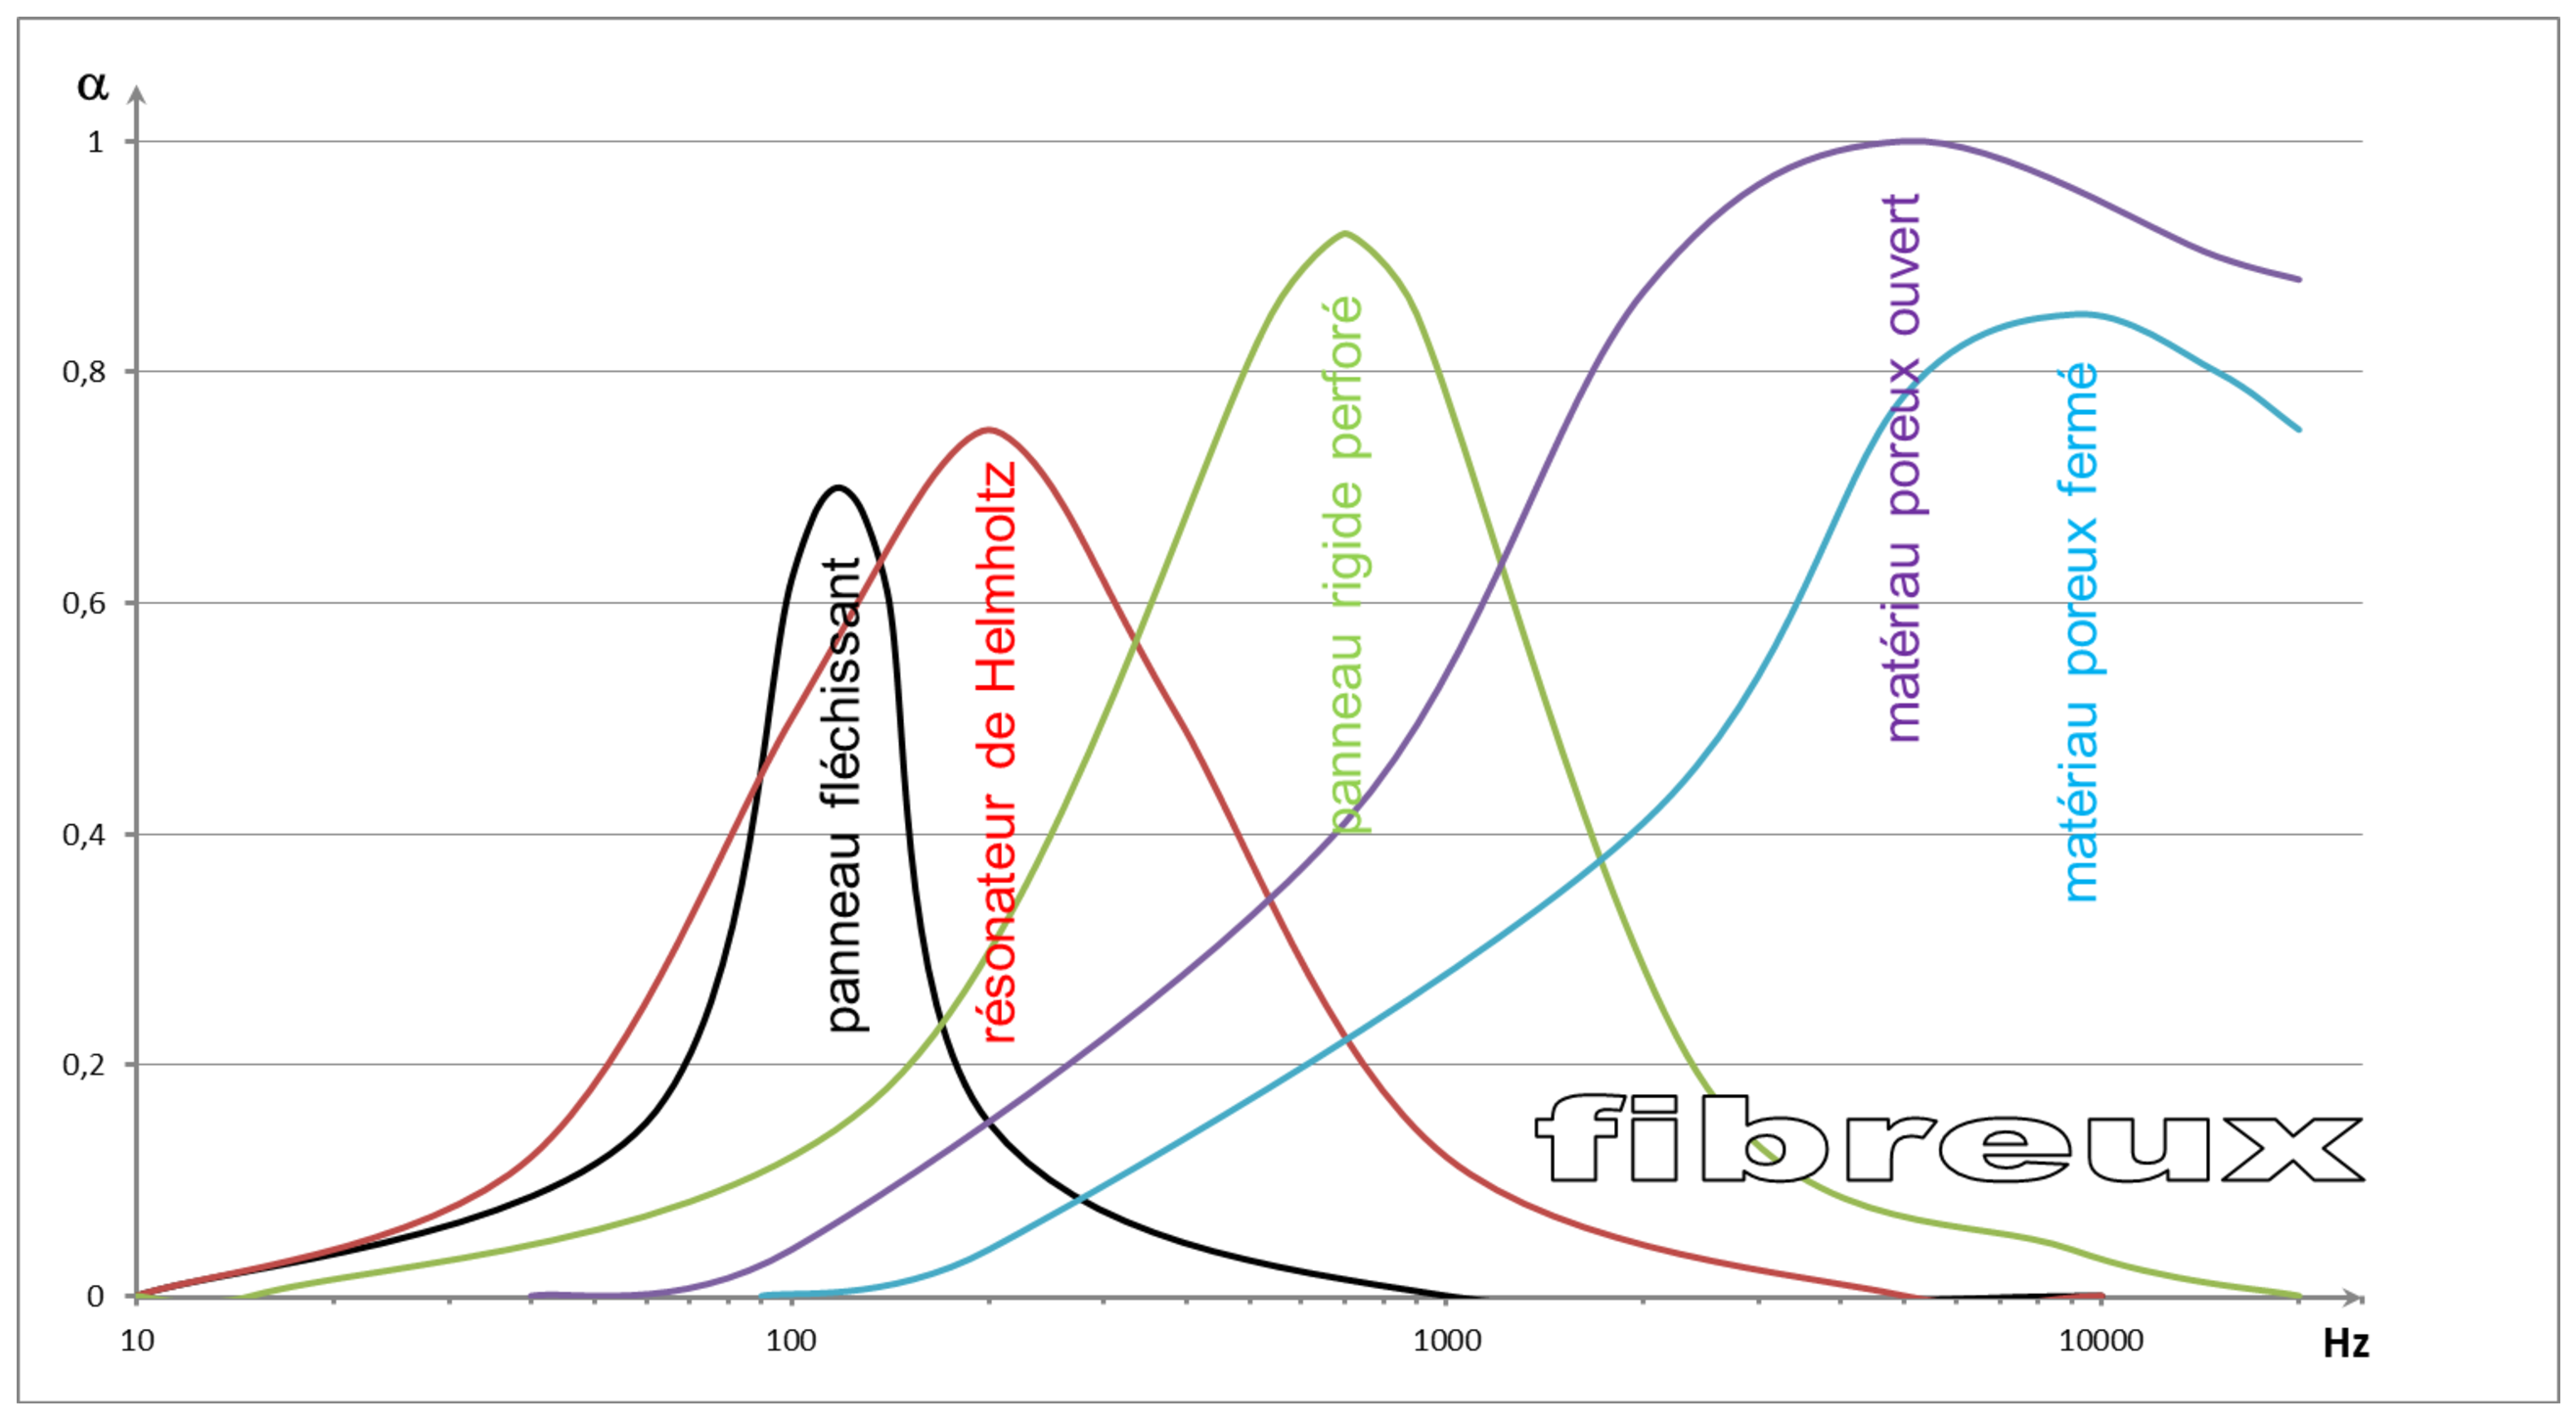
\includegraphics[width=150mm]{Mtx-alpha.eps}
\caption{Coefficient d'absorption pour différents types d'absorbants}\label{Fig-mtxalpha}
\end{figure}

On voit sur la figure~\ref{Fig-mtxalpha} que l'on peut distinguer deux types de comportements:
\begin{itemize}
   \item un comportement d'absorption centré sur une fréquence: il s'agit des panneaux fléchissants, des résonateurs de Helmholtz\index[aut]{Helmholtz (Hermann Ludwig Ferdinand von -), 1821-1894, Allemand} et des panneaux rigides perforés. L'avantage de ces systèmes est qu'ils permettent d'attaquer des fréquences relativement basses. Leur inconvénient est que face à une source large bande, ils ne traitent qu'une infime partie du problème;
  
   \item et un comportement d'absorption large bande: il s'agit des matériaux poreux et fibreux. Bien que n'apportant qu'une absorption très limitée aux basses fréquences, ils permettent de bien traiter le spectre en hautes fréquences et constituent donc une solution simple et aisée à mettre en œuvre. La figure~\ref{Fig-poro}
\begin{figure}[h!]
\centering
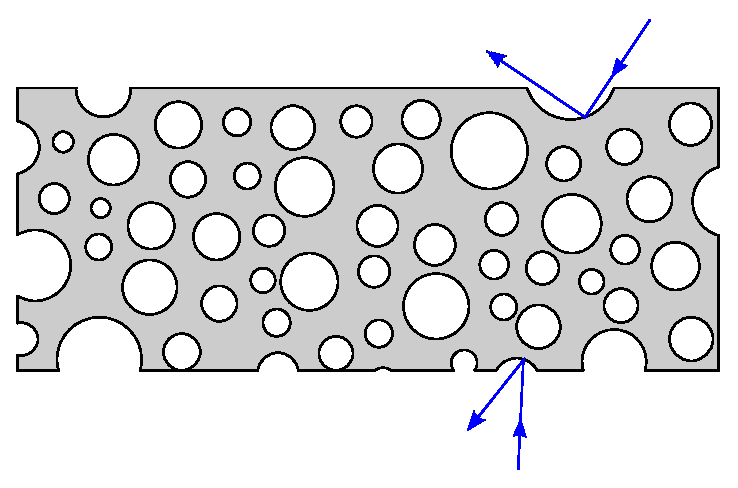
\includegraphics[width=45mm]{poroF.eps}\hspace{4mm}
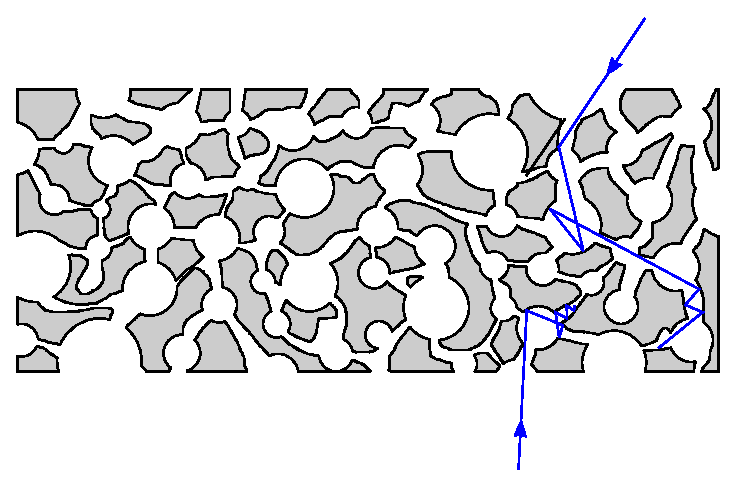
\includegraphics[width=45mm]{poroO.eps}\hspace{4mm}
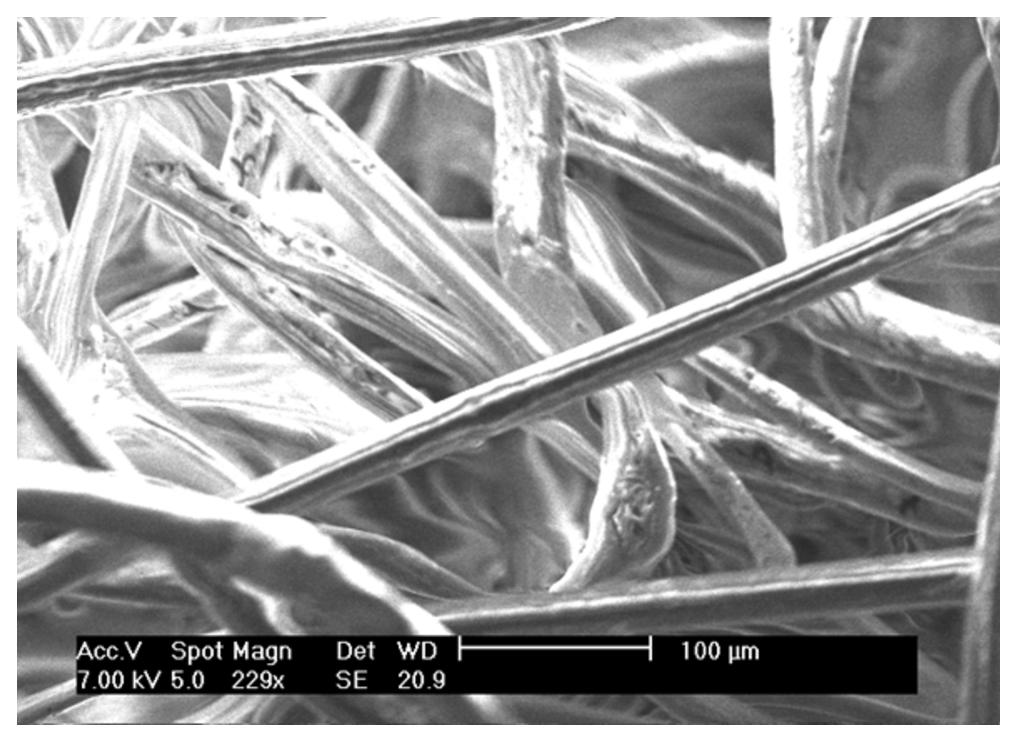
\includegraphics[width=38mm]{fibres.eps}
\caption{Rôle de la porosité}\label{Fig-poro}
\end{figure}
montre le rôle de la porosité dans l'absorption, en augmentant le parcourt moyen parcouru par l'onde acoustique. La dernière photo est une microscopie d'un matériau fibreux réel (on remarquera qu'il y a «beaucoup d'air» et peu de fibres finalement).
\end{itemize}

\medskip
Tout cela justifie la remarque que nous faisons en introduction: la partie difficile à traiter dans les problèmes d'acoustique ne concerne que les basses fréquences où il n'existe que très peu de solutions, surtout simples de mise en œuvre. Les hautes fréquences (supérieures à 2 ou 3000~Hz) peuvent être facilement traitées (poreux, fibreux). De plus, l'oreille humaine, bien que percevant les fréquences de 20 à 20000~Hz, est surtout sensible dans la bande de fréquences allant de 1 à 4~kHz. \textcolorgreen{Dès lors, bien qu'une étude acoustique doive prendre en compte la totalité du spectre (de la source et audible), du point de vue calculatoire (et du point de vue de la conception des solutions), c'est au-dessous de 3000~Hz que le travail devra se concentrer.} Ainsi donc, un traitement par la méthode des éléments finis est tout à fait envisageable pour faire face à la majorité des problèmes: nous entendons par là, avec un «coût» de calcul raisonnable.

\begin{histoire}
\emph{Complément sur le résonateur de Helmholtz.}\\
Les résonateurs de Helmholtz sont une solution très ancienne, puisqu'on utilisait déjà des vases dans les théâtres antiques pour la correction acoustique. Le nom provient d'un dispositif créé dans les années 1850 par Hermann von Helmholtz afin de déterminer la hauteur des différents tons. 

\sbox{\MaBoiteAvecPhotos}{\setlength{\tabcolsep}{0pt}\scriptsize%
\begin{tabular}{c}%
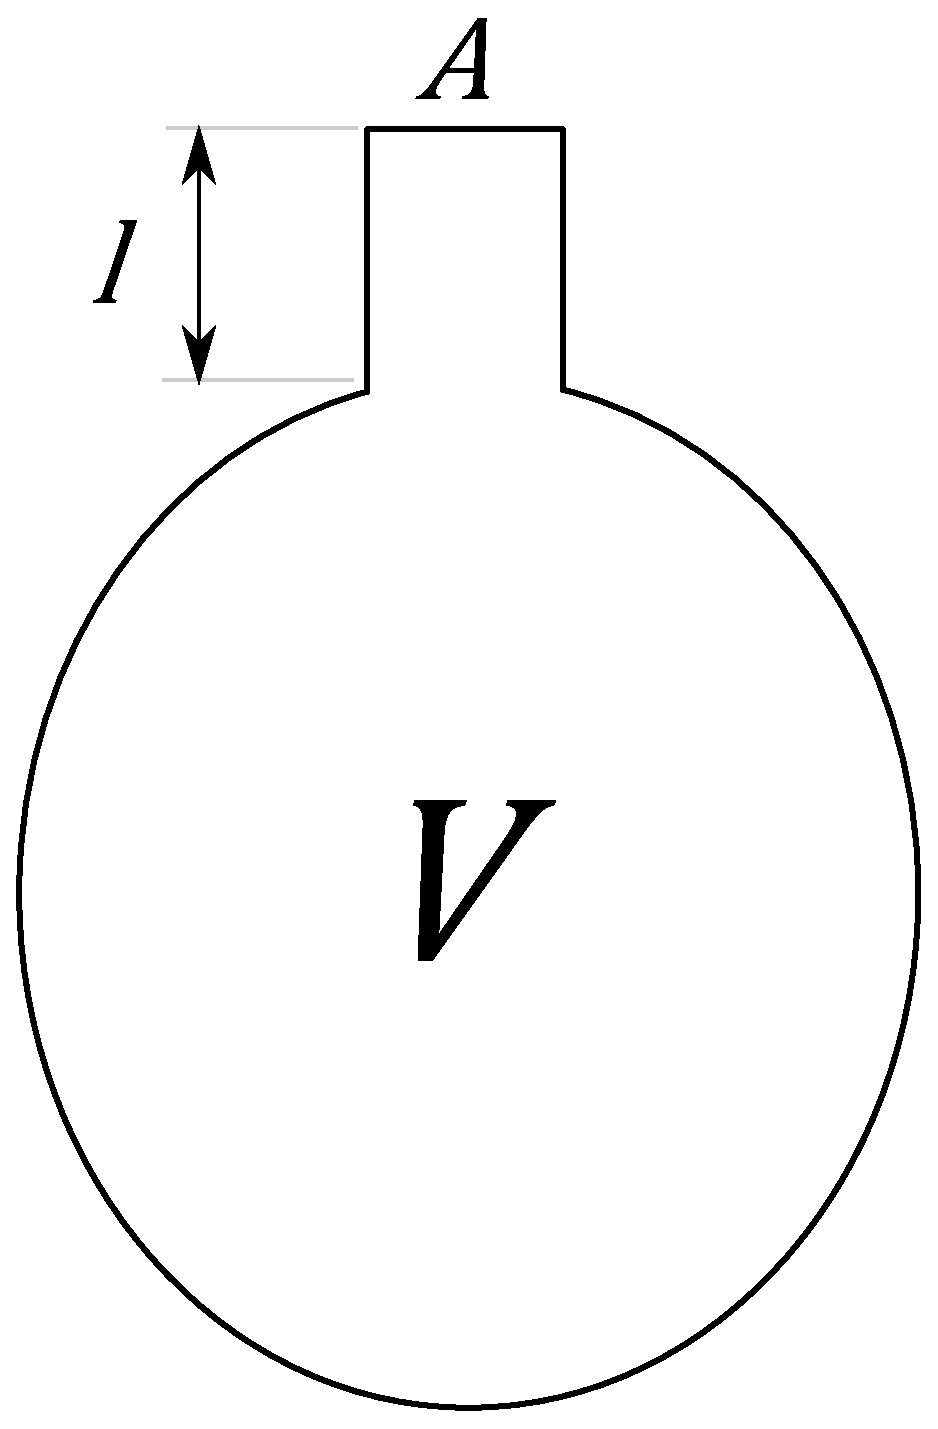
\includegraphics[height=35mm]{Helm.eps}\\
Résonateur de Helmholtz\\[2mm]%
\end{tabular}}
\medskip
\ImageADroite{%
Les applications des résonateurs de Helmholtz sont nombreuses.
En \emph{acoustique des salles}, ils permettent d'atténuer les fréquences médiums.
Le principe du résonateur de Helmholtz est le principe de base permettant de faire des enceintes acoustiques utilisant la technique de l'\emph{enceinte bass-reflex}. L'enceinte contenant le haut-parleur est ouverte par un tube où l'air se déplace et crée donc un résonateur auxiliaire entrant en résonance avec le haut-parleur actif principal permettant d'abaisser la fréquence de coupure basse de l'enceinte.
En \emph{aéronautique}, pour limiter le bruit des réacteurs civils, les nacelles et entrées d'air sont constituées de panneaux sandwich nid d'abeilles recouverts d'une tôle perforée aluminium ou composite. Le résonateur est ainsi constitué par la bouteille (cellule du nid d'abeilles) et le col (perçage de la tôle).
En \emph{automobile}, la résonance de Helmholtz peut être utilisée pour améliorer le remplissage en air des moteurs à combustion interne...}

Le résonateur est assimilé à une cavité fermée de volume~$V$ qui communique avec l'extérieur par l'intermédiaire du col de longueur~$l$ et de section~$A$. On fait par ailleurs l'hypothèse que les dimensions du résonateurs sont petites devant la longueur des ondes acoustiques considérées, que l'air se comporte comme un gaz parfait et que l'on peut négliger les effets thermiques ainsi que les effets dissipatifs. Alors la fréquence du résonateur est:
\begin{equation}
f_0 = \frac{c}{2 \pi} \sqrt{\frac{A}{V l}}
\end{equation}
où~$c$ est la vitesse du son. Ce système se comporte comme un système masse ressort: on se retrouve face aux oscillations libres de l'inertance pneumatique ${\rho A}/{l}$ de la colonne d'air dans le col sur la raideur pneumatique ${\gamma p}/{V}$ de l'air contenu dans la cavité~$V$. Il ne fait pas intervenir la propagation des ondes. La résonance de Helmholtz à la fréquence~$f_0$ doit donc être distinguée des modes propres acoustiques de la cavité, qui sont solutions de l'équation d'Helmholtz, et se situent à des fréquences beaucoup plus élevées que~$f_0$.
\end{histoire}

\medskip
Le coefficient ou facteur d'absorption acoustique est le rapport de l'intensité acoustique qui n'est pas réfléchie (absorbée, propagée et transmise) sur l'intensité acoustique incidente.
On définit le \textcolorblue{coefficient d'absorption de Sabine}~$\alpha_S$,\index[aut]{Sabine (Wallace Clement), 1868-1919, Américain} ou valeur moyenne du coefficient d'absorption, par:
\begin{equation}
\alpha_S = \dfrac{\sum_{i=1}^n\alpha_iS_i}{S_{totale}}
\end{equation}
où la surface totale~$S_{totale}$ est composées de~$n$ surfaces~$S_i$ de coefficient d'absorption~$\alpha_i$.

L'\textcolorblue{aire d'absorption} de chaque surface~$S_i$, quant à elle, est définie par:
\begin{equation}
A_i=\alpha_iS_i
\end{equation}

\medskip
L'\textcolorblue{aire d'absorption équivalente}~$A$ est calculée par la formule de Sabine\index[aut]{Sabine (Wallace Clement), 1868-1919, Américain} datant des années 1898:
\begin{equation}\label{Eq-ASabine}
A = 4mV + \sum^n_{i=1} S_i \alpha_i = 4mV + \sum^{N}_{i=1} A_i
\end{equation}
où~$m$ est l'amortissement du milieu (en général l'air) et~$V$ le volume de la salle (ou du volume) considéré.
Cette formule n'est valable que pour des valeurs de~$\alpha$ sensiblement inférieures à 1. Pour~$\alpha\ge0,3$ on utilisera la formule d'Eyring\index[aut]{Eyring (Carl Ferdinand), 1889-1951, Américain} précisée dans les années 1920, et valable pour toutes les valeurs de~$\alpha$:
\begin{equation}\label{Eq-AEyring}
A = 4mV - \dsum_{i=1}^N S_i \ln(1-\alpha_i)=\dfrac{S_{totale}\overline{\alpha}}{1-\overline{\alpha}}
\end{equation}
où~$\overline{\alpha}$ est le coefficient moyen d'absorption qui peut être pris égale à~$\alpha_S$.

\textcolorgreen{Le terme d'amortissement~$4mV$ est souvent négligé, ce qui est particulièrement licite pour les salles de petite taille.}




\medskip
\subsubsection{Diffraction et réflexion}

La \textcolorblue{diffraction} est un autre phénomène avec lequel il faut compter dans la propagation des ondes. Il est illustré sur plusieurs cas à la figure~\ref{Fig-diffrac}.
\begin{figure}[h!]
\centering
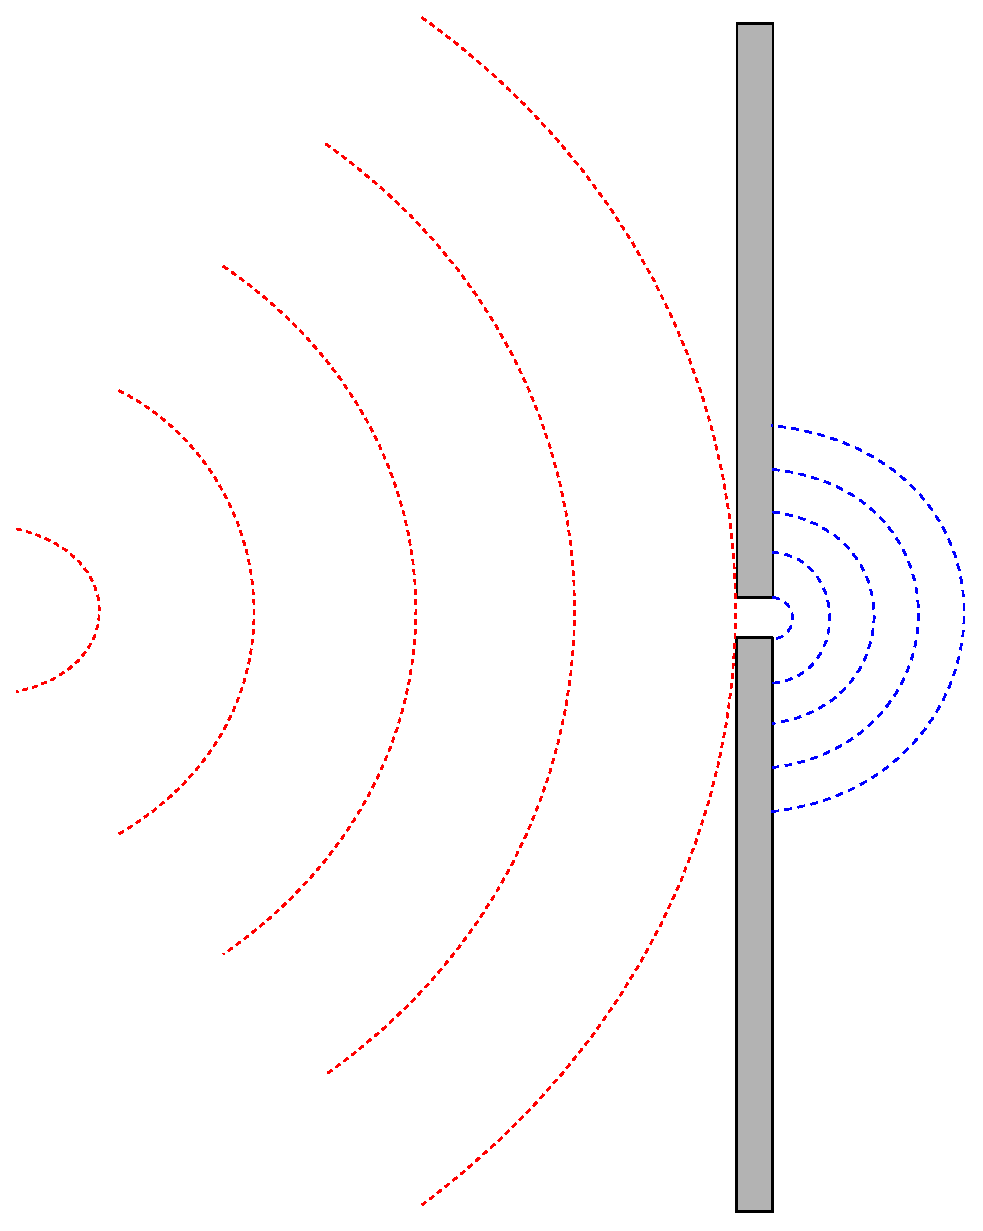
\includegraphics[height=35mm]{diffraction1.eps}\hfill%
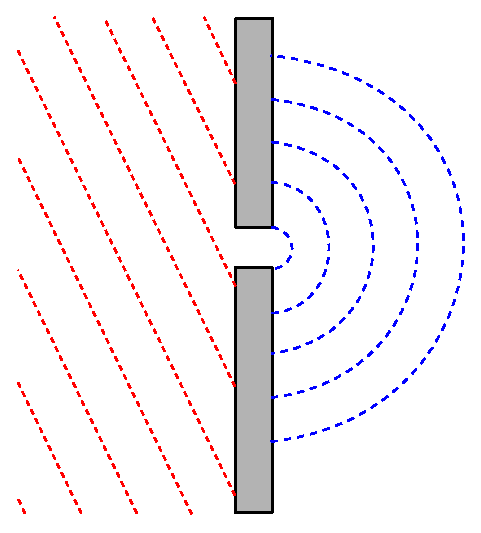
\includegraphics[height=35mm]{diffraction2.eps}\hfill%
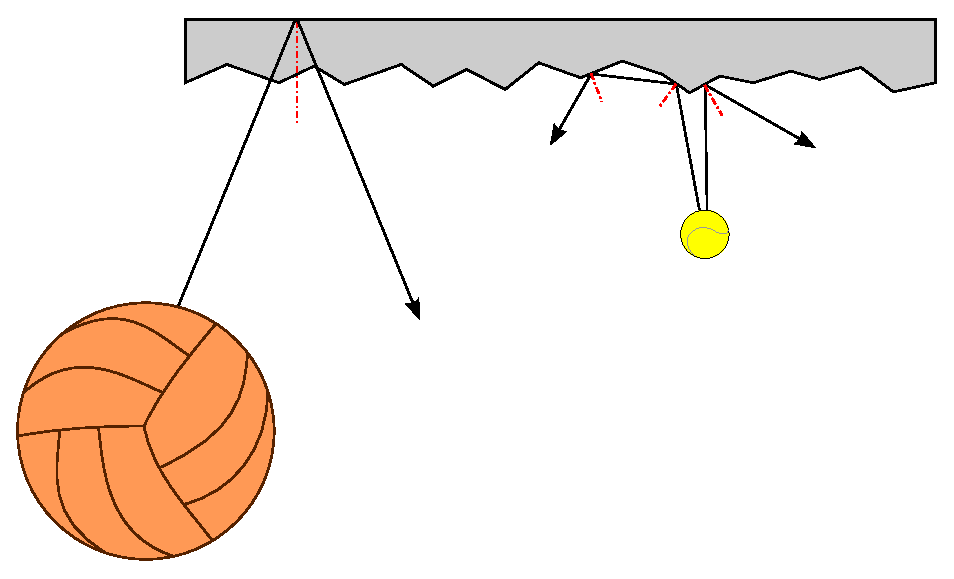
\includegraphics[height=35mm]{diffraction3.eps}\hfill%
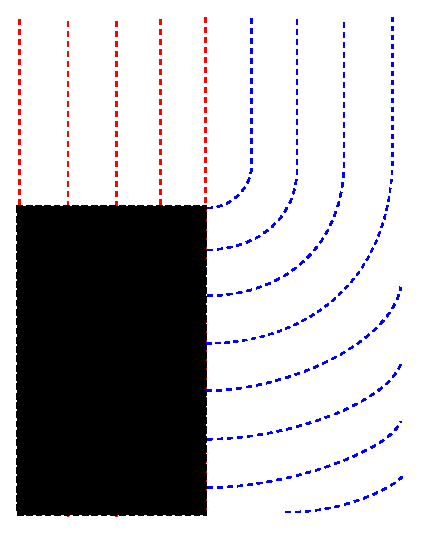
\includegraphics[height=35mm]{diffraction5.eps}\hfill%
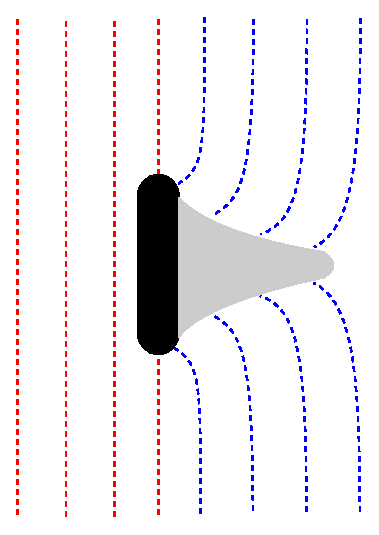
\includegraphics[height=35mm]{diffraction4.eps}
\caption{Phénomène de diffraction}\label{Fig-diffrac}
\end{figure}

Les figures~\ref{Fig-diffrac}a--\ref{Fig-diffrac}c représentent le phénomène de diffraction au travers d'une ouverture. L'onde après l'obstacle, i.e. l'onde diffractée, a la même fréquence, la même longueur d'onde et la même vitesse que l'onde incidente. Par contre, sa direction, son amplitude et sa forme sont modifiées (l'amplitude de l'onde diffractée  est inférieure à celle de l'onde incidente). 

C'est ce phénomène qui fait qu'au coin d'une rue, on entend la personne venant perpendiculairement à nous avant de la voir, comme montré sur la figure~\ref{Fig-diffrac}d.

Rappelons que deux ondes, diffractées ou non (mais ça a plus de sens ici en parlant d'ondes diffractées) peuvent interférer.
Le phénomène analogue se produit également lorsqu'un obstacle est inséré au sein d'un fluide, comme le représente la figure~\ref{Fig-diffrac}e. Les ondes doivent «éviter» l'obstacle, ce qui modifie notamment leur direction sur les bords de l'obstacle.
Il se crée un zone d'ombre en arrière de l'obstacle (schématisée en gris).
De plus, selon la forme de l'objet, les ondes diffractées peuvent générer, plus en aval de l'obstacle, des figures d'interférence.

\medskip
Le phénomène de \textcolorblue{réflexion} sur un obstacle est illustré sur la figure~\ref{Fig-reflex}.
\begin{figure}[h!]
\centering
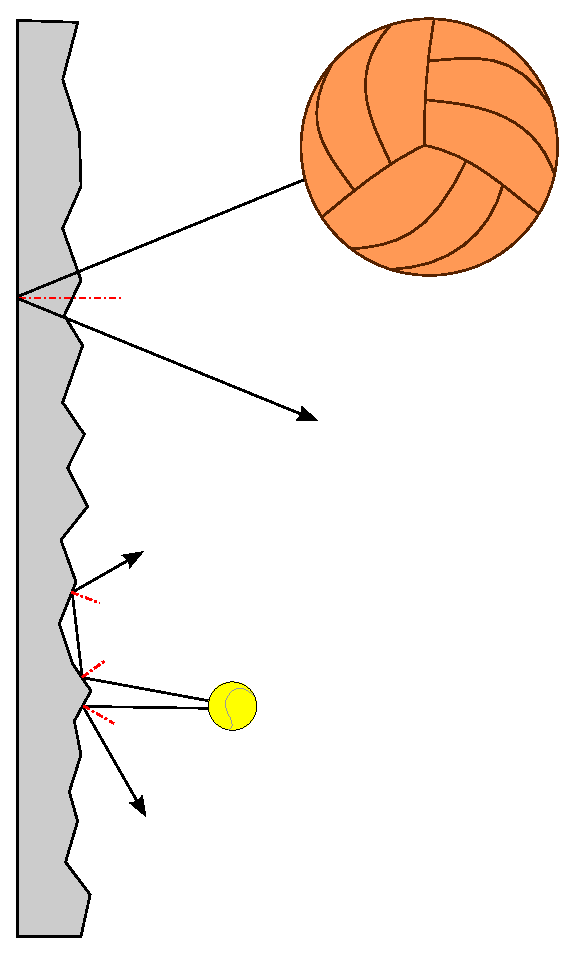
\includegraphics[height=60mm]{reflexion1.eps}\hspace{2cm}
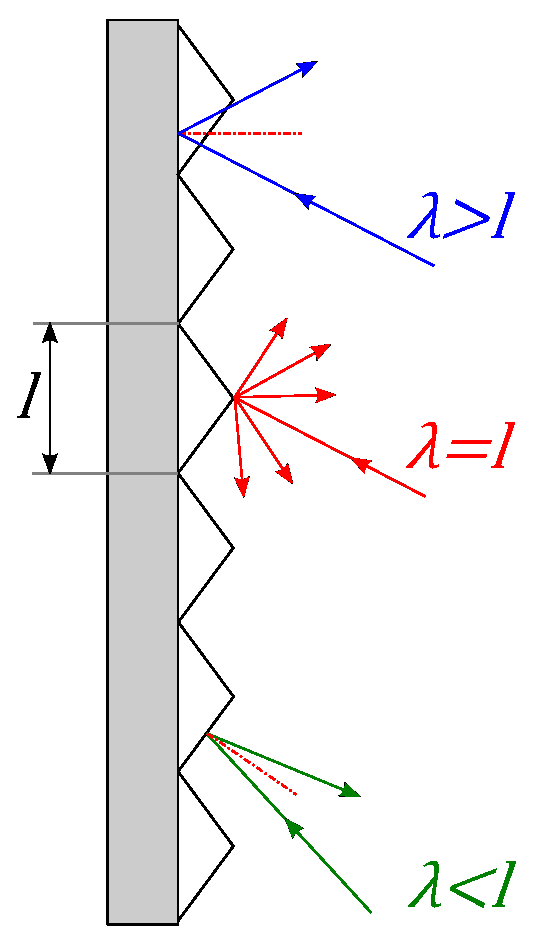
\includegraphics[height=60mm]{reflexion2.eps}
\caption{Phénomène de réflexion}\label{Fig-reflex}
\end{figure}
La figure~\ref{Fig-reflex}a propose une analogie avec des balles, de ce qui est décrit avec des ondes à la figure~\ref{Fig-reflex}b, i.e. le cas de la \textcolorblue{réflexion contre une surface irrégulière}.

Si la balle est grosse face à la taille des irrégularités, i.e. si la longueur d'onde est plus grande que «celle des irrégularités» (ici on a un mur «en accordéon» ayant un motif répétitif de longueur~$l$), alors le trajet est insensible aux irrégularités de la surface: la normale prise en compte est celle de la surface sans irrégularités. Si~$\lambda<l$, alors on peut encore utiliser les lois de l'optique géométrique, mais on voit qu'il est alors nécessaire de disposer d'une discrétisation suffisamment fine pour décrire ces irrégularités. Lorsque la dimension de la balle, i.e. la longueur d'onde de l'onde incidente, s'approche de la longueur caractéristique des irrégularités, alors il convient d'être prudent: si~$\lambda=l$, on a des \textcolorblue{réflexions spéculaires multiples} (on parle aussi de réflexion diffuse) qu'il est souvent difficile de prendre en compte, sauf par des formulation particulières. Souvent, ce cas n'est clairement pas pris en compte.


\medskip
\subsubsection{Environnement ouvert ou fermé}

La propagation d'ondes acoustiques se traite généralement dans deux cas distincts:
\begin{itemize}
   \item celui d'un environnement ouvert, ou champ libre: l'onde peut se propager «à l'infini»;
   \item ou celui d'un environnement fermé: l'onde est confinée dans un volume donné dont elle ne peut sortir.
\end{itemize}

On rappelle par ailleurs qu'une onde voit son intensité décroitre avec la distance parcourue.
\textcolorgris{L'intensité (vectorielle) est le produit de la pression (scalaire) par la vitesse (vecteur).}
Dans les conditions de champ libre, l'intensité acoustique est proportionnelle au carré de la pression acoustique. Quand la distance à la source est doublée, la pression est divisée par deux (et l'intensité acoustique est divisée par quatre). Le niveau de pression acoustique diminue alors de 6~dB.

\medskip
Une question intéressante, dans le cas d'un environnement fermé, est de se demander ce qu'il se passe lorsqu'une source émet à des fréquences qui «n'ont pas la place» de se développer au sein du volume disponible, i.e. \textcolorblue{lorsque les longueurs d'ondes considérées sont supérieures aux dimensions de l'espace dans lequel émet la source}. Ce cas se produit pour les basses fréquences émises par un moteur au sein de son encoffrement, ce dernier étant approximativement un cube de 60~cm de côté.

Et bien, dans ce cas, l'énergie injectée «gonfle» en quelque sorte l'encoffrement. Celui-ci est sollicité en pression... et répond évidemment selon ses \textcolorblue{modes propres}.
Dans de nombreux cas (encoffrement moteur, habitacle de véhicule...), il est nécessaire de prendre en compte la réponse modale du volume dans lequel on définit le problème, car celle-ci influe sur la répartition du champ acoustique, dont notamment d'éventuelles \textcolorblue{résonances}.
\begin{figure}[h!]
\centering
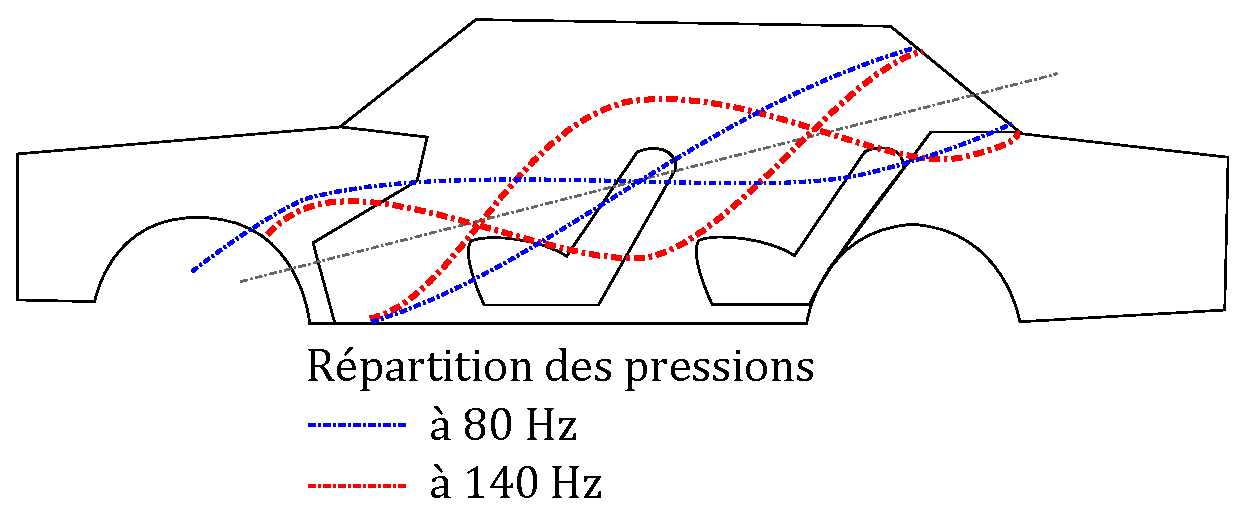
\includegraphics[width=95mm]{modalVh1.eps}\hspace{10mm}%\hfill
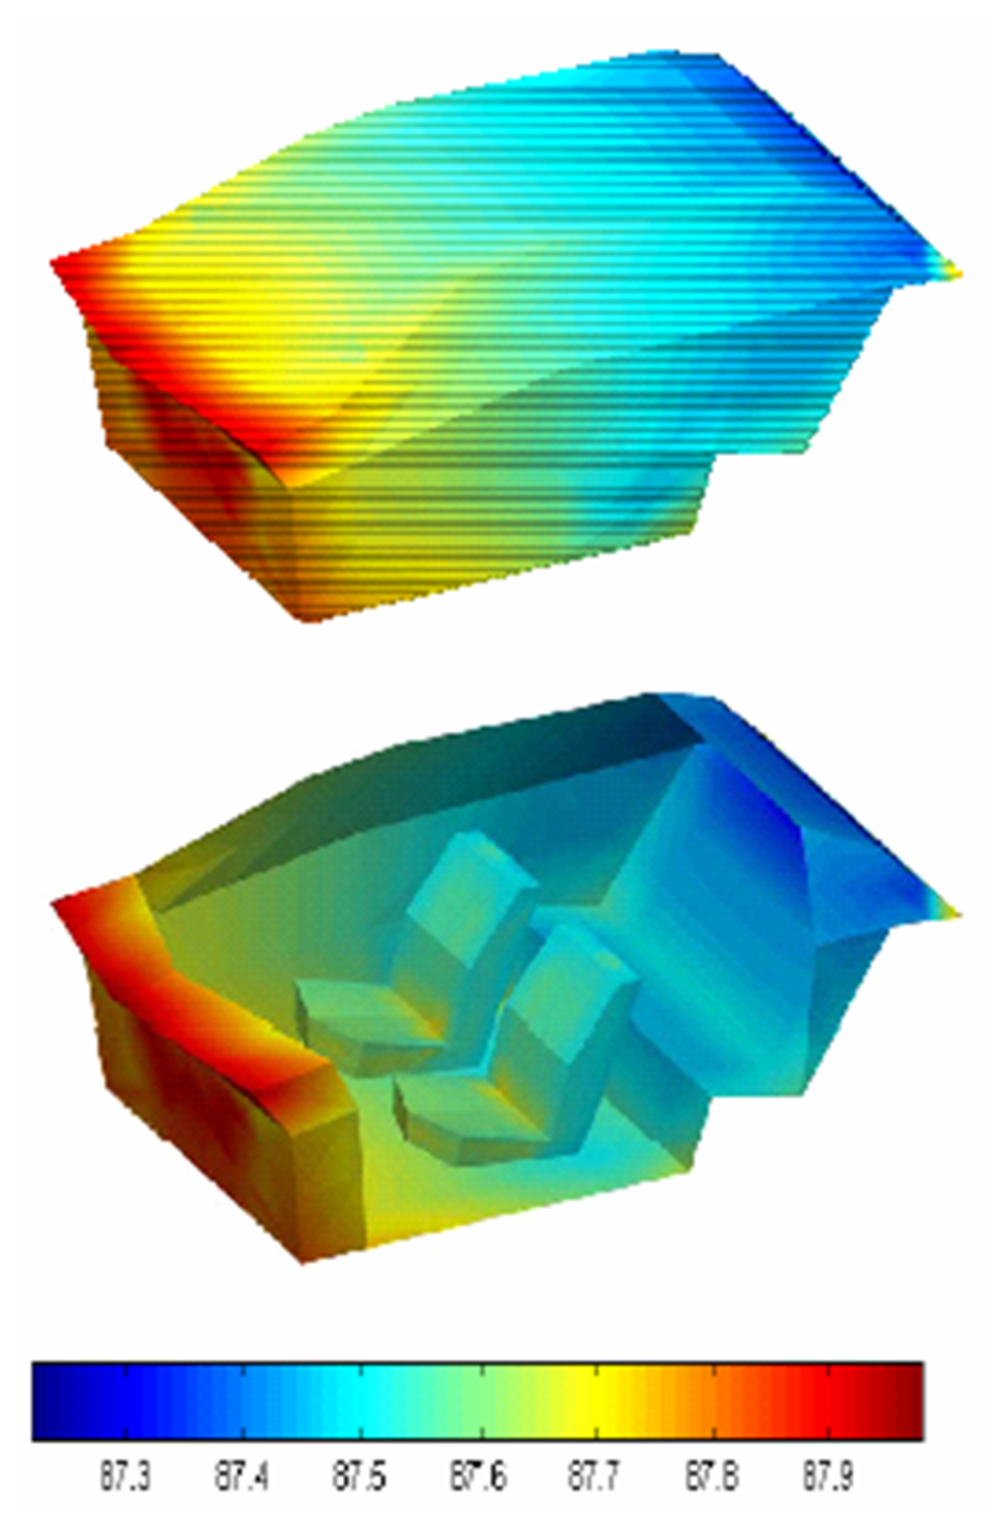
\includegraphics[height=55mm]{modalVh2.eps}
\caption{a) Répartition modale dans un véhicule et b) non-uniformité du champ acoustique}\label{Fig-modalVh}
\end{figure}

Le champ acoustique dans de telles situations (et dans d'autres) est non uniforme, i.e. a des valeurs très différentes d'un point à l'autre.
Ces deux aspects sont illustrés à la figure~\ref{Fig-modalVh}.


%hétérodynage

\medskip
\subsection{Réception}\label{Sec-Reception}

\begin{histoire}
Le bel (B) est utilisé dans les télécommunications, l'électronique et l'acoustique. Vers 1920, les entreprises de téléphonie utilisaient comme unité pour l'atténuation le msc, valant celle d'un mile (1,6 km) de câble standard à la fréquence de 800 Hz. Des ingénieurs des Laboratoires Bell définirent une unité de transmission indépendante du câble et de la fréquence, basée sur dix fois le logarithme décimal. Cette unité s'appela d'abord TU pour «Transmission Unit» (unité de transmission). Elle présentait l'avantage d'être presque équivalente au  msc (1 TU = 1,083 msc). Elle fut renommée décibel en 1923 ou 1924 en l'honneur du fondateur du laboratoire et pionnier des télécoms, Alexander Graham Bell.\index[aut]{Bell (Alexander Graham), 1847-1922, Britannique}

\sbox{\MaBoiteAvecPhotos}{\setlength{\tabcolsep}{0pt}\scriptsize%
\begin{tabular}{c}%
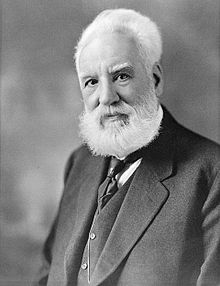
\includegraphics[height=\the\HauteurDesPhotos]{Bell}\\%&%
Bell%
\end{tabular}}
\medskip
\ImageADroite{%
Les Laboratoires Bell consultèrent les opérateurs téléphoniques et administrations responsables. Certaines utilisaient des logarithmes népériens, qui présentent certains avantages pour le calcul, avec une unité appelée le néper (symbole Np). Les deux unités ont coexisté, mais le néper n'a pas connu le succès du décibel. 
La norme ISO 80000-3, page viii, dit d'ailleurs: «L'utilisation du néper est le plus souvent limitée à des calculs théoriques sur des grandeurs de champ, où cette unité est la plus commode, alors que, dans d'autres cas, en particulier pour des grandeurs de puissance, le bel (B), ou en pratique son sous-multiple, le décibel (dB), est largement utilisé. Il convient de souligner que le fait que le néper soit choisi comme l'unité cohérente n'implique pas qu'il convienne d'éviter d'utiliser le bel. Le bel est accepté par le CIPM et l'OIML pour être utilisé avec le SI. À certains égards, cette situation est similaire au fait que l'unité degré (\degre) est utilisée couramment à la place de l'unité SI cohérente radian (rad) pour les angles plans.»}

L'usage du logarithme décimal était d'autant plus pratique qu'avant la diffusion des calculatrices électroniques, on se servait pour les calculs de tables de logarithmes décimaux. Lorsqu'on se propose de calculer l'atténuation dans une ligne de longueur $l$ et de coefficient d'atténuation $\alpha$, il faut élever $(1-\alpha)$ à la puissance $l$. En pratique, on cherchait $l\log(1-\alpha)$ dans la table avant de reconvertir le logarithme en rapport.

\sbox{\MaBoiteAvecPhotos}{\setlength{\tabcolsep}{0pt}\scriptsize%
\begin{tabular}{ccc}%
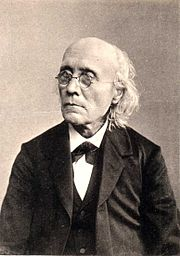
\includegraphics[height=\the\HauteurDesPhotos]{Fechner}&
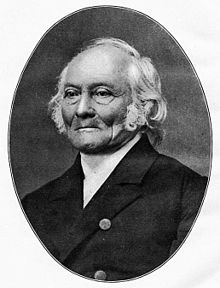
\includegraphics[height=\the\HauteurDesPhotos]{Weber}&
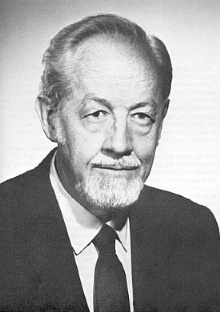
\includegraphics[height=\the\HauteurDesPhotos]{Stevens}\\
Fechner&Weber&Stevens%
\end{tabular}}
\medskip
\ImageAGauche{%
Le décibel a connu un grand succès dans le domaine de l'acoustique. Par une coïncidence fortuite, un décibel, en puissance sonore, correspond à peu près à la plus petite variation perceptible par l'oreille. Selon le philosophe et psychologue Gustav Fechner,\index[aut]{Fechner (Gustav Theodor), 1801—1887, Allemand} la sensation ressentie varierait comme le logarithme de l'excitation. Une unité à progression logarithmique semblait particulièrement pertinente dans un domaine où la perception humaine était en jeu. Des recherches ultérieures sont venues contester la loi de Weber-Fechner,\index[aut]{Weber (Ernst Heinrich), 1795-1878, Allemand} comme la loi de puissance de Stevens\index[aut]{Stevens (Stanley Smith), 1906-1973, Américain} (1951); mais l'usage du décibel s'était établi, même dans des cas où il complique la compréhension.}

La loi de Weber-Fechner stipule que la sensation perçue, $S$, est proportionnelle au logarithme de l'intensité, $I$, du stimulus:
\begin{equation}
 S = k\log(I) 
\end{equation}
alors que la loi de puissance de Stevens modélise cette relation entre ces deux grandeurs par une loi puissance:
\begin{equation}
     S = kI^a 
\end{equation}
où, dans les deux cas, $k$ est une constante.
Stevens a donné des valeurs obtenues pour l'exposant $a$ dans différents domaines dans une publication de 1957 et dans son ouvrage de 1951 \emph{Handbook of Experimental Psychology}.
\end{histoire}

\medskip
\subsubsection{Décibels}

La notion de réception sera forcément liée à une échelle de mesure (une métrique). Nous avons plusieurs fois déjà utilisé le décibel (dB). Toutefois, il convient de distinguer plusieurs échelles:
\begin{itemize}
   \item Le \textcolorblue{décibel} (dB) est une unité de grandeur adimensionnelle définie comme 10 fois le logarithme décimal du rapport entre deux puissances. Pour l'acoustique, ce rapport des puissances est défini entre la grandeur mesurée et une valeur de référence fixée par une norme.
   \begin{equation}
   n \text{(en dB)} = 10 \log_{10} (I_1/I_0)
   \end{equation}
   où $I_1$ et $I_0$ sont deux intensités.
   
   \item Dans la formule précédente, si $I_0$ correspond au seuil de perception ($10^{-12}$~Watt/m$^2$), on obtient les \textcolorblue{décibels absolus ou dB lin ou SPL}. C'est lui que l'on utilise dans les calculs et analyses.
   \begin{equation}
   n \text{(en dB)} = 10 \log_{10} (I_1/10^{-12})
   \end{equation}
   Si $I_1 = 10^{-12}$~Watt/m$^2$ (seuil de perception), on obtient 0~dB.
   Si $I_1 = 1$~Watt/m$^2$ (seuil de douleur), on obtient 120~dB.

   \item Le \textcolorblue{dBA} traduit la perception par l'oreille du phénomène (protection physiologique par filtrage). C'est souvent lui qu'il faut utiliser en lien avec des normes adéquates (fonction du problème considéré) pour savoir s'il y a nuisance sonore ou non.

   \item Il existe d'autres pondérations: le dBC est quasiment linéaire sur plusieurs octaves et est utile pour les mesures subjectives avec de fortes pressions acoustiques. Le dBB est entre le dBA et le dBC. Le dBD est appliqué pour tenir compte de la gêne causée par les sifflements (à hautes fréquences) perçus à l'intérieur des avions modernes. Le dBG est adapté aux basses fréquences...

  \item  Notons que pour être tout à fait exact, que ces pondérations devraient varier avec l'âge: en effet, la perception en fonction de la fréquence et de la puissance varie avec l'âge, ainsi que l'étendue de fréquences audibles (qui diminue, phénomène appelé presbyacousie), comme on le voit sur les courbes (ou diagrammes) de Fletcher\index[aut]{Fletcher (Harvey C.), 1884-1981, Américain} et Munson,\index[aut]{Munson (Wilden A.), 1902-1982, Américain} présentées dans leur article \emph{Loudness, its definition, measurement and calculation} paru en 1933 dans le Journal of the Acoustic Society of America, et que l'on appelle également courbes isosoniques. Fletcher et Munson travaillaient tous les deux aux laboratoires Bell. 
\end{itemize}

\medskip
\subsubsection{Grandeurs acoustiques}

À ce niveau, il convient de rappeler quelques définitions:
\begin{itemize}
   \item La \textcolorblue{pression acoustique} est l'amplitude des variations de la pression en un point de l'espace, par rapport à la pression atmosphérique, provoquées par le passage d'une onde sonore en ce point. (Unité: $N/m^2$)
   \item La \textcolorblue{puissance acoustique} est la quantité (ou le flux) d'énergie acoustique qu'émet une source par unité de temps. (Unité: $W$)
   \item L'\textcolorblue{intensité acoustique} est le flux d'énergie acoustique qui est transmis dans une direction donnée, à travers une unité de surface, pendant une unité de temps. Elle dépend de la puissance de la source, du milieu de propagation, de la distance à la source. (Unité: $W/m^2$)
\end{itemize}

\medskip
L'intensité acoustique s'exprime comme:
\begin{equation}
I = \frac{p^2}{Z}
\end{equation}
où $p$ est la pression acoustique et $Z$ l'\textcolorblue{impédance} (Unité: $Ns/m^3$).

\begin{remarque}
Dans le cadre de mesures:
\begin{itemize}
   \item l'intensité acoustique est représentée par la puissance électrique (Watt);
   \item la pression acoustique est représentée par la tension électrique (V) \textcolorgris{(la tension électrique fournie par un microphone est proportionnelle à la pression acoustique $p$)};
   \item l'impédance acoustique est représentée par la résistance électrique.
\end{itemize}
On peut remplacer $I = p^2/Z$ par $P = V^2/R$ et en déduire la \textcolorblue{puissance moyenne}:
\begin{equation}
P_{moy}=\dfrac{V_1^2+...+V_n^2}{nR}
\end{equation}
On définit aussi la \textcolorblue{tension efficace ou tension RMS} (Root Mean Square), qui est la tension continue qui donnerait une puissance continue égale à la puissance moyenne. On a donc $P_{moy}=V_{eff}^2/R$, soit:
\begin{equation}
V_{eff}=\sqrt{\dfrac{V_1^2+...+V_n^2}{n}}
\end{equation}
\end{remarque}

\medskip
Notons que l'on «parle» souvent, dans le monde des acousticiens, en termes de bandes de fréquence, l'analyse en bandes fines n'étant utilisée que pour des analyses plus poussées.

L'octave étant le doublement de la fréquence~$f_2=2f_1$, le \textcolorblue{tiers d'octave} est défini par un rapport entre les fréquences de~$f_2=2^{1/3}f_1$. 
   
Les fréquences centrales de l'analyse par tiers d'octave normalisée sont les suivantes
(en Hz): 20, 25, 31, 40, 50, 63, 80, 100, 125, 160, 200, 250, 315, 400, 500, 630, 800, 1000, 1250, 1600, 2000, 2500, 3150, 4000, 5000, 6300, 8000, 10000, 12500.

\medskip   
Le \textcolorblue{bruit blanc}  est un son dont le spectre contient toutes les fréquences à la même amplitude. Une analyse à bande de fréquence constante donnerait donc une courbe constante égale à 1.
   
Le \textcolorblue{bruit rose} est un bruit dont le niveau par bande d'octave est constant. Ce signal se rapproche plus de la sensibilité de l'oreille que le bruit blanc. Pour cette raison, le bruit rose est donc souvent utilisé dans l'univers audible pour calculer
la réponse fréquentielle d'une chaîne de reproduction sonore.

\medskip
\subsubsection{Impédance}

La notion d'impédance mérite que nous y passions quelques instants. En effet, elle nous permettra par la suite de définir des conditions aux limites pour nos modèles numériques.

%VM : paragraphe ci-dessous BOF et peut-être mal placé
L'impédance caractéristique d'un milieu (solide, liquide ou gazeux) est définie comme le rapport de la pression acoustique sur la vitesse de déplacement en milieu ouvert (i.e. en l'absence d'ondes réfléchies). C'est une propriété du matériau considéré qui est égale, dans le cas d'un espace illimité, au produit de la masse volumique du matériau par la vitesse du son dans ce même matériau.

\medskip
L'impédance acoustique dans les solides est définie par:
\begin{equation}
Z = \dfrac{F}{v}=\rho c
\end{equation}
où~$F$ est la force ($N$), $v$ la vitesse de déplacement ($m/s$), $\rho$ la densité linéique du milieu ($kg/m$) et $c$ la vitesse de propagation ($m/s$).
On remarquera que~$c$ et~$v$ sont inversement proportionnelles.
Dans les solides, la vitesse de propagation est plus élevée que dans les gaz et l'énergie s'y dissipe moins rapidement: l'onde peut se propager plus loin.

\medskip
L'impédance acoustique dans les gaz est définie par:
\begin{equation}
Z = \dfrac{p}{v}=\rho c
\end{equation}
où cette fois~$p$ est la pression acoustique ($Pa$), les autres grandeurs étant les mêmes qu'auparavant.

\colorgreen
\begin{remarque}[Quelques valeurs]
L'impédance de l'air vaut $Z=413,5$ (en~$Pa.s/m$ ou~$N.S/m^3$) à 20\degre C. Elle varie avec la température, tout comme la densité et la célérité du son.

La vitesse du son dans l'air en $m/s$ vaut $c=331,5+0,6\theta$, où~$\theta$ est la température de l'air en \degre C (elle varie également en fonction de la pression atmosphérique et de la température).

L'impédance acoustique de l'eau est d'environ~$1,5.10^6 ~Pa.s/m$.
\end{remarque}\colorblack

Considérons deux milieux d'impédances respectives~$Z_1$ et~$Z_2$, et une onde incidente se propageant dans le milieu 1 jusqu'à arriver à sa frontière avec le milieu 2.
Si $Z_1=Z_2$, alors l'onde incidente se propage intégralement dans le milieu 2, i.e. elle est intégralement transmise.
Par contre, si $Z_1\ne Z_2$, alors l'onde incidente se scinde en une onde réfléchie et une onde transmise. L'amplitude de l'onde réfléchie est d'autant plus grande que la discontinuité entre les deux milieux est marquée.
On définit alors le \textcolorblue{coefficient de réflexion} par:
\begin{equation}
\dfrac{p_r}{p_i}=\dfrac{Z_2-Z_1}{Z_2+Z_1}
\end{equation}
où les indices~$r$ et~$i$ désignent l'onde réfléchie et l'onde incidente respectivement.

\medskip\colormagenta{\small 
Supposons qu'une onde se propage dans l'air ($Z_1=413,5$) et rencontre un solide tel que $Z_2=500 000$. Alors le coefficient de réflexion est de 99,8\%.
Dans le cas où une onde passe d'un milieu plus dense à un milieu moins dense, le coefficient de réflexion devient négatif.%: «la compression s'est réfléchie en raréfaction».}

\medskip\colorblack
Deux cas extrêmes nous intéressent:
%VM illustrer ces 2 cas. Cas2=paroi fixe...
\begin{itemize}
   \item la \textcolorblue{réflexion à une extrémité libre}: dans ce cas,~$Z_2\approx0$ et la vitesse de l'extrémité est~$v=2v_i$. On assiste à un changement de signe de $v_r$ sans renversement de la forme de l'onde.
   \item la \textcolorblue{réflexion à une extrémité fixe}: dans ce cas,~$Z_2\rightarrow\infty$ et la vitesse de l'extrémité est $v=0$. Il n'y a pas de changement de signe de~$v_r$, mais la forme de l'onde est renversée.
\end{itemize}







%slides VM p27
\medskip
\subsubsection{Normes, indices et psycho-acoustique}

De très nombreuses normes et grandeurs existent dans le domaine de l'acoustique, correspondant à des problématiques différentes. Nous en listons quelques unes ci-dessous, mais cette liste est très loin d'être exhaustive:
\begin{itemize}
   \item Le \textcolorblue{comportement acoustique} d'une salle diffère selon la zone de fréquence considérée.
   
Pour les longueurs d'ondes supérieures au double de la plus grande dimension d'une pièce: le son se comporte de manière équivalente aux changements de pression de l'air statique.
Pour les longueurs d'onde comparables aux dimensions de la pièce: il y a dominance des modes propres de la salle. Il y a amplification des fréquences, ce qui «colore» le son et création d'ondes stationnaires.
Pour des longueurs d'ondes inférieures à la moitié des dimensions de la salle: on est dans le cas de réflexions multiples, et on peut faire une équivalence lumineuse et utiliser les méthodes de tir de rayons.

   \item L'une des premières grandeurs à connaître est le \textcolorblue{bruit ambiant}. Son niveau maximal est fixé en fonction de la destination du local.

   \item Une seconde grandeur particulièrement fondamentale pour la caractérisation de locaux, quelque soit leur destination, est le \textcolorblue{temps de réverbération} ou TR.  Il correspond à l'intervalle de temps nécessaire pour que la pression acoustique (d'une salle) diminue à un millième de sa valeur initiale suite à l'arrêt de la source sonore. Cela représente une diminution du niveau sonore de 60~dB. Le temps de réverbération indique la capacité qu'à la salle à réverbérer les sons.
   
En 1898, Sabine\index[aut]{Sabine (Wallace Clement), 1868-1919, Américain} découvrit que le temps de réverbération~$T_R$ était proportionnel au volume de la salle~$V$ et inversement proportionnel à la surface équivalente d'absorption~$A$:
   \begin{equation}
    T_R = \frac{k V}{A} 
   \end{equation}
où la constante de proportionnalité~$k$, trouvée initialement égale à 0,161, vaut~$k=(24\ln10)/340 =0,163$~s/m, et où l'aire d'absorption équivalente est calculée par la formule de Sabine~(\ref{Eq-ASabine}) ou d'Eyring~(\ref{Eq-AEyring}).\index[aut]{Eyring (Carl Ferdinand), 1889-1951, Américain}

Selon la destination du local, plusieurs normes existent pour mesurer le TR. De plus, la destination du local joue également sur la valeur acceptable ou non du TR.

Le \textcolorblue{Early Decay Time} (EDT) est le temps de décroissance sur les 10 premiers dB. Il est subjectivement plus important, car il se rapproche de l'impression de réverbération alors que le TR fait référence aux propriétés du local.

   On utilise également le \textcolorblue{taux de décroissance spatiale}~$DL$, et plus particulièrement le taux de décroissance par doublement de distance~$DL_2$.

   \item La \textcolorblue{Clarté} dépend de la distribution temporelle de l'énergie précoce, de la densité temporelle, du niveau des réflexions et de la nature du message sonore. 
   L'\textcolorblue{intelligibilité de la parole} est conditionnée par le TR, le rapport signal/bruit, le volume et la géométrie de la pièce, et la répartition des surfaces réfléchissantes et absorbantes.
   Plus le temps de réverbération est court, meilleure sera la compréhension de la parole, à moins que le bruit de fond ne domine.
   Plusieurs indicateurs seront à prendre en compte: le \textcolorblue{rapport Signal-Bruit} (S/B), le \textcolorblue{Speech Transmission Index} (STI), le \textcolorblue{Percentage Articulation Loss of Consonants} (\%-Alcons), le \textcolorblue{RApid Speech Transmission Index} (RASTI)...
   \begin{align*}
   \text{Clarté sur 80~ms: } & C_{80}=10\log_{10}\dfrac{\int_0^{80}p^2(t)\dd t}{\int_{80}^\infty p^2(t)\dd t}\\
   \text{Distinctness sur 50~ms: } & D = \dfrac{\int_0^{50}p^2(t)\dd t}{\int_{0}^\infty p^2(t)\dd t}\\
   \text{Temp central: } & T_c = \dfrac{\int_0^\infty tp(t)\dd t}{\int_0^\infty p(t)\dd t}\\
   \text{Articulation Loss Consonent: } & ALC=\dfrac{200 r^2T_R^2}{VQ}\\
   \text{RApid Speech Transmission Index: } & RASTI =
   \left\{\begin{array}{ll}
   0 & \text{ si } (S/B)_{app}\le 15\\
   1 & \text{ si } (S/B)_{app}\ge 15\\
   \frac{(S/B)_{app}+15}{30}
   \end{array}
   \right.\\
   & \text{ avec } (S/B)_{app}=\frac19\sum_{i=1}^9 (S/B)_i
   \end{align*}
   où~$Q$ est le facteur de directivité.   
   Des relations empiriques sont également utilisées:
   \begin{align*}
    ALC &\approx 170,5 e^{-592 STI} \\
    STI &\approx -0,18 \ln(ALC) + 0,95
   \end{align*}

   \item De là, on peut définir les \textcolorblue{rayons de discrétion et de confidentialité}...
   
   \item D'autres indicateurs existent liés par exemple à la spatialisation (InterAural Cross Correlation (IACC), Lateral Efficienty (LE)...) ou a des critères de sonorisation (clarté locale, homogénéité...).
   
   \item Des indicateurs prennent également en compte la \textcolorblue{durée d'exposition} au bruit, surtout évidemment dans le cadre de la législation du travail.
    Ainsi 80~dBA pendant 8~heures correspondent à 86~dBA pendant 2~heures, 90~dBA pendant 45~min, 95~dBA pendant 15~min, 100~dBA pendant 5~min, 107~dBA pendant 1~min ou 115~dBA pendant 28~s.
    
    le $L_{ex,d}$ est le \textcolorblue{niveau d'exposition sonore quotidienne} exprimé en dBA pour des bruits stables ou fluctuants.
    Le $L_{pc}$ est le \textcolorblue{niveau de pression crête} exprimé en dBC pour une exposition à des bruits impulsionnels.
    
%   \item Pré qualification des locaux selon la norme NFS 31080
%   \item Recommandations INRS
%   \item norme  NF S31080

   \item L'Organisation Internationale de Normalisation (ISO) a proposé plusieurs courbes qui correspondent toutes à un certain degré de confort acoustique (ou de gêne): courbes d'évaluation du bruit, ou courbes de \textcolorblue{Noise Rating} (NR). Grâce à ces courbes, il est possible de déterminer au moyen d'un seul chiffre le niveau de pression acoustique maximum autorisé. Les indices N40 et N80 sont souvent pris en référence.

   \item Dans \emph{Éléments de physiologie et de pathologie des bruits}, Wisner\index[aut]{Wisner (Alain), 1923-2004, Français} définit trois seuils de bruit correspondant à un indice de gêne subjective: lorsque le bruit ambiant est en zone 1, le travail intellectuel n'est pas gêné de façon appréciable; lorsque le bruit ambiant est en zone 2, le travail intellectuel est pénible, le travail courant n'est pas gêné de façon appréciable; lorsque le bruit ambiant est en zone 3, le travail intellectuel est extrêmement pénible, le travail courant est difficile; et lorsque le bruit ambiant est situé en zone 4, une exposition prolongée peut conduire à la surdité.

   \item La Sonie ou bruyance (loudness) est une quantification de la perception du son chez l'être humain. C'est une grandeur psycho-acoustique qui se rattache de façon complexe à la pression acoustique. Les courbes isosoniques issues des travaux de Fletcher et Munson % VM, puis de Zwicker entre autres, 
   expriment la relation entre la fréquence d'un stimulus sonore continu et la perception de sa sonie. L'ISO a donné un tracé normalisé afin de pouvoir définir le phone, unité de l'expression de la sonie.

   \item Il est toujours possible de construire d'autres métriques pour des problèmes particuliers. Par exemple dans \cite{bib-VM-suav}, on trouvera une métrique adaptée à la mesure de la «beauté» des bruits périodiques.
\end{itemize}

\medskip
\section{Calculs acoustiques par éléments finis}\label{Sec-AcouMEF}

\medskip
\subsection{Modèles simplifiés pour valeurs de référence}

Dans ce petit paragraphe, nous donnons quelques formules simples.
Elles permettent néanmoins d'effectuer un prédimensionnement rapide pour les salles acoustiques et/ou de disposer de quelques valeurs (au moins leur ordre de grandeur) vers lesquelles des calculs plus complexes doivent conduire.

\medskip
\subsubsection{Puissance de la source sonore et propagation}

En champ libre, on a la loi de propagation pour le champ direct suivante:
\begin{equation}
L_p=L_w+10\log_{10}\left(\dfrac{Q}{4\pi d}\right)
\end{equation}
où~$L_p$ (en dBA) est le niveau de pression sonore du champ direct, $L_w$ le niveau de puissance de la source, $d$ la distance à la source et~$Q$ le facteur de directivité ($Q=1$ source omnidirectionnelle, $Q=2$ source omnidirectionnelle posée sur le sol...).

\medskip
Dans une salle (suffisamment réverbérante), on constate que le champ est diffus, et alors on a:
\begin{equation}
L_p = L_w + 6 - 10\log_{10} A
\end{equation}
où~$L_p$ (en dBA) est le niveau de pression sonore du champ diffus, $L_w$ le niveau de puissance de la source et~$A$ l'aire équivalente d'absorption.
On remarque que~$L_p$ est constant quelle que soit la distance à la source (puisqu'on est en hypothèse de champ diffus) et qu'il ne dépend que de~$A$, i.e. de la capacité d'absorption disponible dans la salle.
On notera que les parois, surtout si elles sont légères, présentent une certaine transparence et qu'il est bon, pour ajuster le modèle, d'augmenter l'aire d'absorption de la proportion d'énergie qui quitte la salle par transmission (défaut d'isolation).

\medskip
En terme de modélisation, cela signifie qu'à proximité d'une source (jusqu'à environ 30cm), on considérera que l'on est en champ direct. Au-delà, on utilisera la relation correspondant au champ réverbéré.



\medskip
\subsubsection{Modes d'une salle}

Pour les longueurs d'onde de l'ordre des dimensions de la salle, il y a prédominance des modes propres de la salle. Il faut donc pouvoir les évaluer.
Pour un salle parallélépipédique de dimensions~$L$, $l$ et~$h$, les fréquences de résonance sont données par:
\begin{equation}
f_{(i,j,k)} = \frac{c}2\sqrt{\left(\frac{i}{L}\right)^2+\left(\frac{j}{l}\right)^2+\left(\frac{k}{h}\right)^2}
\end{equation}
Les modes~$(i,0,0)$, $(0,j,0)$ et~$(0,0,k)$ sont des modes axiaux dans la directions de~$L$, $l$ et~$h$ respectivement, les modes~$(i,j,0)$, $(0,j,k)$ et~$(i,0,k$ les modes tangentiels, et les modes~$(i,j,k)$ les modes obliques.
La pression acoustique se met sous la forme:
\begin{equation}
p(x,y,z) = \dsum_i\dsum_j\dsum_k p_{ijk}\cos\left(\frac{i\pi}{L}x\right)\cos\left(\frac{j\pi}{l}y\right)\cos\left(\frac{k\pi}{h}z\right)
\end{equation}

La formule de Maa (1939) donne le nombre~$N(f)$ de fréquences propres inférieures ou égales à une fréquence donnée~$f$:
\begin{equation}
N(f) = \frac{4\pi}{3}V\left(\frac{f}{c}\right)^3 + \frac{\pi}{4}S\left(\frac{f}{c}\right)^2 + \frac{L_t}{8}V\left(\frac{f}{c}\right)
\end{equation}
où~$V=Llh$ est le volume de la salle, $S=2(Ll+Lh+lh)$ est la surface totale des parois de la salle, et~$L_t=4(L+l+h)$ est la longueur totale des arêtes de la salle.

En dérivant la formule de Maa par rapport à la fréquence, on peut déterminer la
densité de fréquences propres à une fréquence donnée, i.e. le nombre de fréquences propres comprises dans un intervalle de 1~Hz centré sur~$f$:
\begin{equation}
\dd N(f) = \frac{4\pi V}{c^3}f^2 + \frac{\pi S}{2c}f + \frac{L_t}{8c}
\end{equation}

Pour une salle non parallélépipédique, on peut, sauf géométrie vraiment très biscornue, utiliser les relations précédentes en considérant le parallélépipède le plus proche de la géométrie réelle.

\medskip
\subsubsection{Remarques}

On n'oubliera pas de prendre en compte les pertes par transmission dans le calcul des coefficients d'absorption.

\medskip
Dans le cas où l'on s'intéresse à la transmission entre plusieurs salles, il faudrait effectivement ne pas oublier qu'une salle n'a pas que des sources internes, mais également des sources externes correspondant à ce qui a pu s'échapper des autres salles, ou de ce qui rayonne suite à la propagation de vibrations.

\medskip
C'est une lapalissade, mais dans un calcul global, les phénomènes locaux (écrantage...) ne sont pas pris en compte (ou alors de manière globale)...
Si l'on s'intéresse au niveau moyen résultant dans un local, prendre en compte la totalité des surfaces absorbantes, qu'elles soient situées au murs, au plafond ou sous formes d'écrans, de fauteuils... fonctionne.
Par contre, si l'on a besoin de descendre dans le détail local de la répartition de la pression acoustique (par exemple répartition poste à poste), alors il convient d'utiliser des méthodes plus adéquates, dont les éléments finis, que nous allons présenter maintenant.

\medskip
\subsection{Constitution d'un modèle éléments finis}

Si l'on ajoute des termes de sources, alors l'équation des ondes~(\ref{Eq-EqOndeAcou}) devient:
\begin{equation}\label{Eq-OndeSrc}
\dfrac{1}{\rho c^2}\dfrac{\partial^2p}{\partial t^2}+\nabla.\left(-\dfrac{1}{\rho}(\nabla p-q)\right)=Q
\end{equation}
dont l'inconnue est toujours la pression acoustique et où~$q$ et~$Q$ représentent les termes de sources pour un dipôle et un monopôle respectivement.
Pour les milieux dispersifs, un terme de dissipation supplémentaire peut être introduit dans l'équation des ondes qui devient:
\begin{equation}
\dfrac{1}{\rho c^2}\dfrac{\partial^2p}{\partial t^2}-d\dfrac{\partial p}{\partial t}+\nabla.\left(-\dfrac{1}{\rho}(\nabla p-q)\right)=Q
\end{equation}
Dans la suite, on restera dans le cas~$d=0$.

Dans le cas harmonique, l'équation~(\ref{Eq-OndeSrc}) devient l'équation d'Helmholtz~(\ref{Eq-Helm})\index[aut]{Helmholtz (Hermann Ludwig Ferdinand von -), 1821-1894, Allemand} avec termes sources:
\begin{equation}
-\dfrac{\omega^2p}{\rho c^2}+\nabla.\left(-\dfrac{1}{\rho}(\nabla p-q)\right)=Q
\end{equation}
Si l'on souhaite introduire le d'amortissement dans l'équation, alors les quantités~$c$ et~$\rho$ peuvent être complexes (au sens appartiennent à~$\CC$). Par exemple, pour un modèle d'amortissement de Rayleigh,\index[aut]{Rayleigh (John William Strutt, troisième baron -), 1842-1919, Anglais} la célérité $c$ est une combinaison linéaire de la masse et de la raideur.


\medskip
Pour réaliser notre modèle de calcul vibro-acoustique par éléments finis, nous devrons disposer de sources et de conditions aux limites:
\begin{itemize}
   \item La source est généralement modélisée par un \textcolorblue{monopôle} ou un \textcolorblue{dipôle}. Un monopôle est une source omnidirectionnelle, alors qu'un dipôle représente une source ayant deux directions opposées selon lesquelles le champ est plus fort. Un dipôle peut être vu comme deux monopôles de même puissance séparés par une petite distance et en opposition de phase. On peut également utiliser des quadripôles si besoin.
   On trouve également parfois des sources ponctuelles, linéaires ou ayant d'autres formes prédéfinies.
   
   \item La \textcolorblue{condition de Neumann} correspond à une condition de  \textcolorblue{mur rigide}. Elle définit une frontière sur laquelle la composante normale de l'accélération est nulle (mur immobile parfaitement réfléchissant):
   \begin{equation}\label{Eq-muracou}
   -n.\left(-\frac1{\rho}(\nabla p-q)\right)=0
   \end{equation}
	S'il n'y a pas de dipôle (i.e. $q=0$) et si la densité du fluide est constante (i.e. $\rho=cte$), alors l'équation précédente devient:
	\begin{equation}
	\dfrac{\partial p}{\partial n}=0
   \end{equation}	   
   i.e. la dérivée de la pression par rapport à la normale est nulle.
   
   Dans certains codes, on peut spécifier la valeur de l'accélération normale, i.e. le second membre de l'équation~(\ref{Eq-muracou}) n'est plus nul mais vaut~$a_n$ (condition de Neumann relevée), qui représente alors une source externe. Cela permet également de coupler de manière faible l'acoustique à une calcul structural: un premier calcul de structure permet de déterminer le vibrations d'une surface, et cette-ci est introduite ensuite dans le calcul acoustique. Le \textcolorgreen{couplage est donc faible} car dans ce cas on fait l'hypothèse que l'acoustique en retour ne modifie pas (ou peu) la vibration de la structure. De manière inverse, on a également couplage faible si le fluide agit sur le solide et que celui-ci en retour n'agit que peu sur le fluide.
   
   \item La \textcolorblue{condition de Dirichlet} correspond à une \textcolorblue{condition d'absorption parfaite}. Elle est telle que la pression acoustique s'annule sur la surface:
   \begin{equation}
   p=0
   \end{equation}
   En général, dans les codes, une telle condition permet de mettre la pression à zéro, ou à toute autre valeur (condition de Dirichlet relevée) définie par l'utilisateur. Le second membre n'est alors plus nul mais vaut~$\overline{p}$. Cela permet de modéliser une source débitant une pression constante (applicable sur un nœud si besoin).
   
   \item La \textcolorblue{condition de Robin} correspond à une \textcolorblue{condition d'impédance}. Elle se situe entre les deux cas précédents:
   \begin{equation}
   \begin{array}{rll}
   -n.\left(-\dfrac1{\rho}(\nabla p-q)\right)
   &=-\dfrac{i\omega p_t}{Z} \text{ en analyse harmonique, ou }\\
   &=\dfrac{1}{Z}\dfrac{\partial p_t}{\partial t} \text{ en analyse temporelle}   
   \end{array}
   \end{equation}
   Lorsque~$Z\rightarrow\infty$ on retrouve le cas du mur rigide, et lorsque~$Z\rightarrow0$ celui de l'absorption parfaite.
   
   Pour les \textcolorgreen{plaques perforées}, on utilisera cette condition pour gérer l'absorption. Certains logiciels calculent l'impédance à notre place en fonction de paramètres physiques tels que: la viscosité dynamique, l'épaisseur et la porosité (diamètre des trous, distance entre trous, ou aire des trous et résistance de passage au fluide) et la réactance du panneau.
   
   \item L'absorption peut être gérée par l'impédance, mais certains logiciels incluent des \textcolorgreen{modèles de fluides équivalent} (homogénéisation), dont le plus connu est celui de Biot-Allard.\index[aut]{Biot (Maurice Anthony), 1905-1985, Américain}\index[aut]{Allard (Jean-François), ?-, Français} Il concerne les matériaux poreux et nécessite de connaître leur porosité, résistance au passage de l'air, tortuosité, et longueurs caractéristiques visqueuse et thermique (ces deux derniers paramètres ayant une influence moins importante que les trois premiers sur l'absorption). D'autres modèles existent comme le modèle de Johnson-Champoux-Allard, celui de Johnson-Champoux-Allard-Lafarge...
   
   \item Les \textcolorblue{conditions aux limites en rayonnement} permettent de définir les régions par lesquelles les ondes peuvent quitter le modèle. On trouve généralement des conditions de radiation plane, cylindrique et sphérique.
   \item De la même manière on trouve des \textcolorblue{conditions de rayonnement}, plane ou cylindrique, permettant de modéliser une source, i.e. une onde qui arrive (et non plus une onde qui quitte le modèle).
   
   \item Lorsque le couplage faible décrit plus haut n'est pas suffisant, il faut alors intégrer le \textcolorblue{couplage fort} fluide-structure au calcul: le fluide, définit par ses champs de pression et de vitesse exerce des forces de type aérodynamique (de pression) sur la structure. Cette force aérodynamique se met sous la forme $F = \frac12 \rho v^2SC$, où~$v$ est la vitesse, $S$ la «surface de référence» (pour nous cette surface de référence sera la surface mouillée)\footnote{Dans le cas d'étude aérodynamiques et pour les corps bien profilés, la surface de référence sera la projection de la surface dans un plan orthogonal à la direction selon laquelle on veut le résultat.
   
   Toujours dans ce cas, on décompose la force aérodynamique selon trois axes en une force de traînée~$F_x$ parallèle à la direction moyenne de l'écoulement; une force de dérive~$F_y$ perpendiculaire à la direction moyenne de l'écoulement, dans le plan horizontal; et une force de portance~$F_z$, perpendiculaire à la direction moyenne de l'écoulement, dans le plan vertical.} et~$C$ le coefficient aérodynamique. En retour, le déplacement et/ou la déformation de la structure affecte, au moins localement, le champ de l'écoulement fluide et par conséquent la direction et l'intensité des charges aérodynamiques: ce \textcolorblue{cycle des interactions} entre le fluide et la structure est la caractéristique du couplage fort entre les deux milieux, i.e. \textcolorblue{chaque milieu influe significativement sur l'autre}.
   \textcolorgreen{Basiquement, on retiendra que l'analyse acoustique fournit un chargement (la pression acoustique) à l'analyse structurelle, et l'analyse structurelle fournit des accélérations à l'analyse acoustique.}

Si l'on ne peut pas découpler les équations de chaque milieu (c'est parfois possible et ça vaut donc le coût d'essayer), alors on essaye généralement de procéder par la méthode dite «décalée»: chaque physique est traitée séparément, et l'on essaye ensuite de faire transiter l'information d'un code à l'autre, ce qui n'est pas toujours simple, engendre des erreurs numériques supplémentaires, et surtout nécessite de développer des algorithmes de couplage. Sinon, la méthode dite «monolithique» est théoriquement la plus optimale puisque le fluide et la structure sont traités par un même code de calcul. Toutefois, lorsque les géométries ou la physique du problème à traiter deviennent complexes ce type de méthode n'est plus envisageable puisque chaque milieu (fluide ou solide) nécessite des procédures de calcul numérique spécifiques.
Notons que certains codes de calcul gèrent de manière assez simple pour l'utilisateur ce couplage entre différentes physiques.

   \item La \textcolorblue{continuité de la pression} à l'interface entre deux milieux peut être à entrer. Il suffit de spécifier que le saut est nul:
   \begin{equation}
   -n.\left[\left(-\dfrac1{\rho}(\nabla p-q)\right)_1 - \left(-\dfrac1{\rho}(\nabla p-q)\right)_2\right] =0
   \end{equation}
\end{itemize}



\medskip
\subsection{Convergence}

La convergence d'un calcul acoustique dépend non seulement de la taille du maillage, mais également de la taille du pas de temps.

\medskip
\subsubsection{Discrétisation en espace}
Le maillage doit être en mesure de prendre en compte les longueurs d'ondes qui nous intéressent dans le calcul. Les ondes doivent pouvoir «se développer» dans le calcul, et pour cela, on utilisera la condition simple suivante:
\begin{equation}
h=\dfrac{k\lambda}{10}
\end{equation}
où~$h$ est la taille de la maille, et~$k$ le degré de l'approximation utilisée dans l'élément.
\textcolorgreen{Ainsi $h=\lambda/10$ pour un élément linéaire, et $h=\lambda/5$ pour un élément quadratique.}

\medskip
\subsubsection{Discrétisation en temps}

La condition de Courant,\index[aut]{Courant (Richard), 1888-1972, Américain} Friedrichs\index[aut]{Friedrichs (Kurt Otto), 1901-1982, Allemand} et Lewy\index[aut]{Lewy (Hans), 1904-1988, Américain} (condition CFL), énoncée dans leur article de 1928 \cite{bib-CFL}, définit, au travers d'un nombre adimensionnel appelée nombre de Courant~$C$, une condition de convergence pour résoudre certaines équations aux dérivées partielles, notamment les équations aux dérivées partielles hyperboliques, utilisant la méthode des différences finies. Pratiquement, il sert à donner le seuil dimensionnel sous lequel on observe une instabilité de calcul, erreur d'approximation dans des calculs numériques, grandissant rapidement au fur et à mesure des calculs. \textcolorgreen{Si la dimension de la grille est inférieure à la distance parcourue dans l'intervalle de pas de temps par l'onde la plus rapide que permet l'équation, l'erreur grandit et envahit la solution physique.}

\medskip
Le nombre de courant~$C$, pour un problème de dimension~$n$ en espace (et $1$ en temps), est défini par:
\begin{equation}
C = \Delta t \sum_{i=1}^n\frac{u_{x_i}}{\Delta x_i} \leq C_{max}. 
\end{equation}
où~$u$ est la fonction inconnue du problème, $\Delta t$ le pas de temps et $\Delta x_i$ le pas de discrétisation de chaque variable spatiale.

La constante $C_{max}$ prend différentes valeurs en fonction de la méthode utilisée pour résoudre l'équation discrétisée.
Pour une méthode explicite, on utilisera $C_{max} = 1$, alors que pour une méthode implicite, moins sensible aux instabilités numériques, on pourra prendre une valeur plous grande pour~$C_{max}$.
On fera en sorte de prendre~$C_{max}$ le plus grand possible pour la méthode considérée, ce qui permettra par conséquent de calculer le pas de temps le plus grand possible (la taille de la discrétisation en espace étant contrainte par les fréquences visées) afin de minimiser les calculs.


\medskip
\subsection{Vers l'infini...}

Lorsque l'on fait un calcul en champ ouvert... il faudrait définir le domaine jusqu'à l'infini.
Généralement, on définit une zone (par exemple sphérique ou hémisphérique) entourant le problème, située à une distance suffisante, et permettant de simuler l'infini: ce qui nous intéresse est donc une condition d'absorption parfaite.
Nous avons déjà mentionné la condition de Dirichlet.
Toutefois, elle n'est pas optimale.

Décrite pour la première fois en 1994 par Jean-Pierre Bérenger\index[aut]{Bérenger (Jean-Pierre), ?-, Français} dans \emph{A perfectly matched layer for the absorption of electromagnetic waves}, une \textcolorblue{zone absorbante parfaitement adaptée} (en anglais Perfectly matched layer ou PML) est une zone absorbante artificielle pour les équations d'ondes, couramment utilisée pour tronquer les domaines de calcul dans les méthodes numériques de simulation de problèmes à frontières ouvertes, particulièrement dans les méthodes FDTD et FEM.
La propriété essentielle d'une PML qui la distingue d'un matériau absorbant ordinaire est le fait qu'elle est conçue de telle sorte que les ondes incidentes l'atteignant depuis un matériau non PML ne se réfléchissent pas à l'interface. Cette propriété permet aux PML d'absorber fortement toutes les ondes sortant d'un domaine de calcul sans les renvoyer dans ce domaine.

Cette approche a été modifiée puis généralisée en ce que l'on appelle la stretched-coordinate PML. Les PML correspondent à une transformation dans laquelle une ou plusieurs coordonnées sont attachées à des nombres complexes; plus techniquement, il s'agit en réalité d'une prolongation analytique de l'équation d'onde dans le domaine complexe, où les ondes propagatives (oscillantes) sont remplacées par des ondes dont l'amplitude décroît exponentiellement. Ce point de vue permet aux PMLs d'être adaptées aux matériaux inhomogènes comme les guides d'ondes, ainsi qu'à d'autre systèmes de coordonnées et d'équations d'ondes.

La PML amortit une certaine longueur d'onde existant dans le système, déduite de la fréquence et d'une célérité de référence des ondes.
Dans le cas d'un problème uniquement fluide, cette célérité de référence sera prise égale à la vitesse du son. Dans le cas d'ondes se propageant dans un solide, on la prendra égale à la vitesse de compression du son. Pour un modèle couplé fluide-structure, on pourra prendre une valeur moyenne entre les deux précédentes comme estimation initiale. Pour une onde dont le vecteur d'onde fait un angle~$\theta$ avec la direction dans laquelle on veut absorber, il faudrait prendre une valeur de~$1/\cos|\theta|$.


\medskip
\subsection{... et au-delà}

Si l'on souhaite savoir ce qu'il se passe loin de la source, en dehors du domaine de simulation (sans devoir tout mailler), alors il est possible d'utiliser des techniques dites de \textcolorblue{champ lointain} (Far Field).

L'idée est somme toute assez simple: disposant des informations (pression, directivité) sur la surface d'un volume donné dans lequel est décrit le problème, il est possible d'extrapoler le comportement en dehors de ce volume sous certaines hypothèses, notamment de non réflexion du champ (par exemple champ libre). La mise en œuvre, quant à elle, est loin d'être aussi simple que l'idée.

Certains logiciels de calcul offrent cette possibilité.


\medskip
\subsection{Post-Traitement}

La pression~$p(x,y,z)$ calculée est un pression complexe (i.e. appartenant à~$\CC$).
Toutefois, il est aisé, à partir de celle-ci, de définir un certain nombre d'autres valeurs d'intérêt:
\begin{itemize}
   \item $p(x,y,z,t)=\Re\left(p(x,y,z)e^{i\omega t}\right)$;
   \item $p_{rms}(x,y,z)=\dfrac{1}{\sqrt{2}}|p(x,y,z)|$;
   \item $SPL(x,y,z)=20\log_{10}\left(\dfrac{p_{rms}(x,y,z)}{p_{ref}}\right)$;
   \item d'autres grandeurs liées au modèle. Souvent on définira, à partir des données et des résultats le facteur de perte. Par exemple, on peut le définir par:
   \begin{equation}\label{Eq-FacPerte}
   D_{tl} = 10\log_{10}\left(\dfrac{W_i}{W_t}\right)
   \end{equation}
   où~$W_i$ est la puissance moyenne incidente et~$W_t$ la puissance moyenne transmise.
\end{itemize}
Définir toutes ces quantités ne nécessite pas de refaire le calcul éléments finis. Elles ont donc un coût de calcul quasiment nul! Il ne faut donc surtout pas se priver de définir les quantités les plus parlantes pour le problèmes considéré.

\medskip
\section{Quelques illustrations}\label{Sec-AcouIllus}
%http://svn.parisson.org/castax/

\medskip
\subsection{Un exemple en acoustique des salles}

L'acoustique des salles d'une manière générale peut se passer de couplage. Seul le volume de la salle est à discrétiser. Les zones d'absorption situées en parois seront modélisées par leur impédance, ainsi que les pertes par transmission. Dans le cas d'un locuteur, la source sera ponctuelle.

La figure~\ref{Fig-AcouSalle} présente une salle et sa modélisation.
\begin{figure}[h!]
\centering
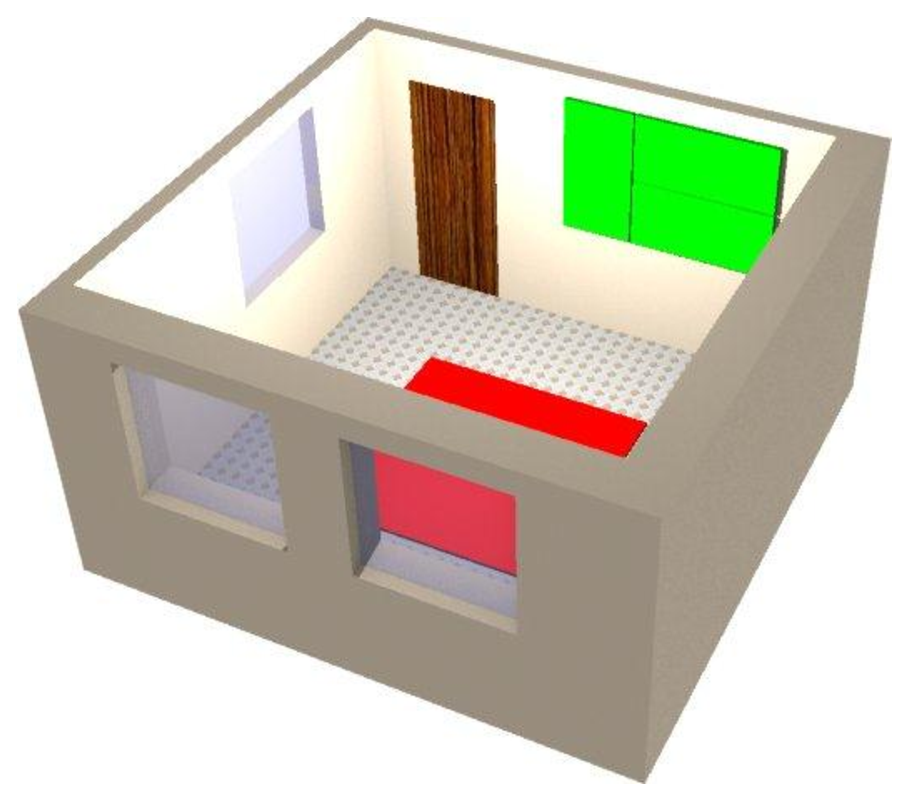
\includegraphics[width=66mm]{AcouSalle1.eps}\hspace{10mm}
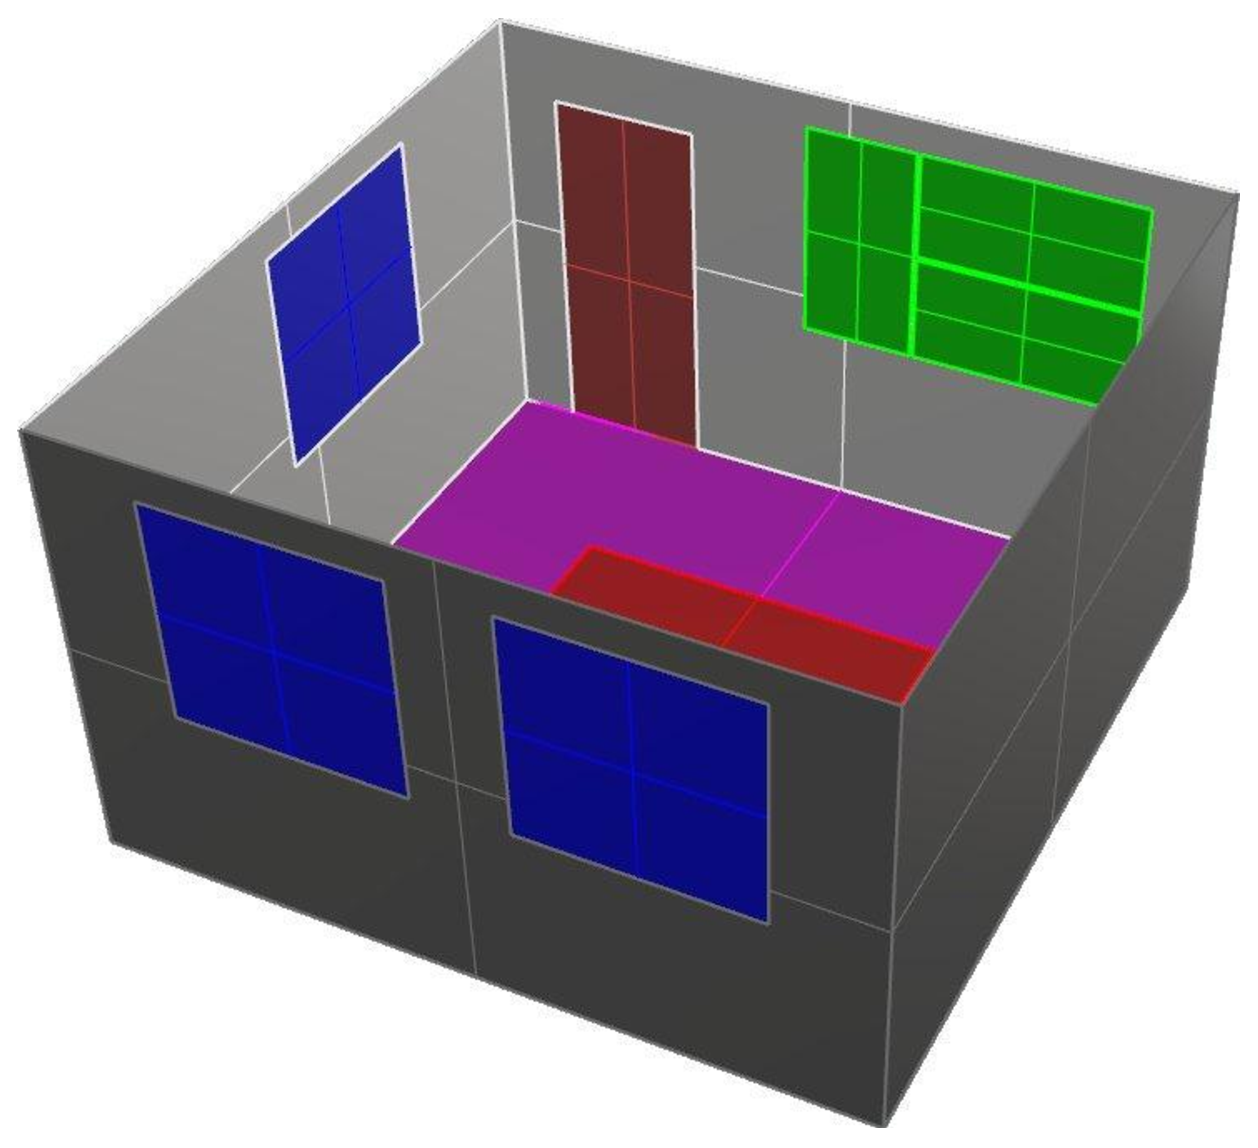
\includegraphics[width=65mm]{AcouSalle2.eps}
\caption{Un problème d'acoustique des salles}\label{Fig-AcouSalle}
\end{figure}
La salle est constitué de deux murs épais en béton, de deux murs fins en placo. Elle comporte 3 fenêtres et une porte. Le sol est en carrelage, avec au centre un tapis épais. Le plafond non représenté est en béton. Au mur, à côté de la porte, se trouvent trois panneaux acoustiques.

Pour effectuer la modélisation, on ne contentera de représenter les surfaces internes de la pièce. Les murs épais (en gris foncé), le sol et le plafond seront considérés comme parfaitement réfléchissants. Pour les murs fins, on entrera une impédance correspondant à la perte par transmission. On fera de même avec les fenêtres et la porte. Les conditions d'absorption des panneaux acoustiques et de la moquettes pourront être modélisées en entrant l'impédance associée ou en utilisant un modèle d'absorption de type Biot-Allard si cela est disponible dans le logiciel.

On maillera le volume d'air intérieur défini par ces surfaces portant les conditions aux limites. On n'oubliera pas d'ajouter la source: ici un locuteur sera représenté par un monopôle, i.e. une source ponctuelle omnidirectionnelle. On lancera l'analyse en fréquences et l'on s'intéressera par exemple à la répartition spatiale de la pression acoustique à différentes fréquences choisies.


\medskip
\subsection{Un silencieux automobile}

La figure~\ref{Fig-AcouSilen} présente un silencieux d'automobile.
\begin{figure}[h!]
\centering
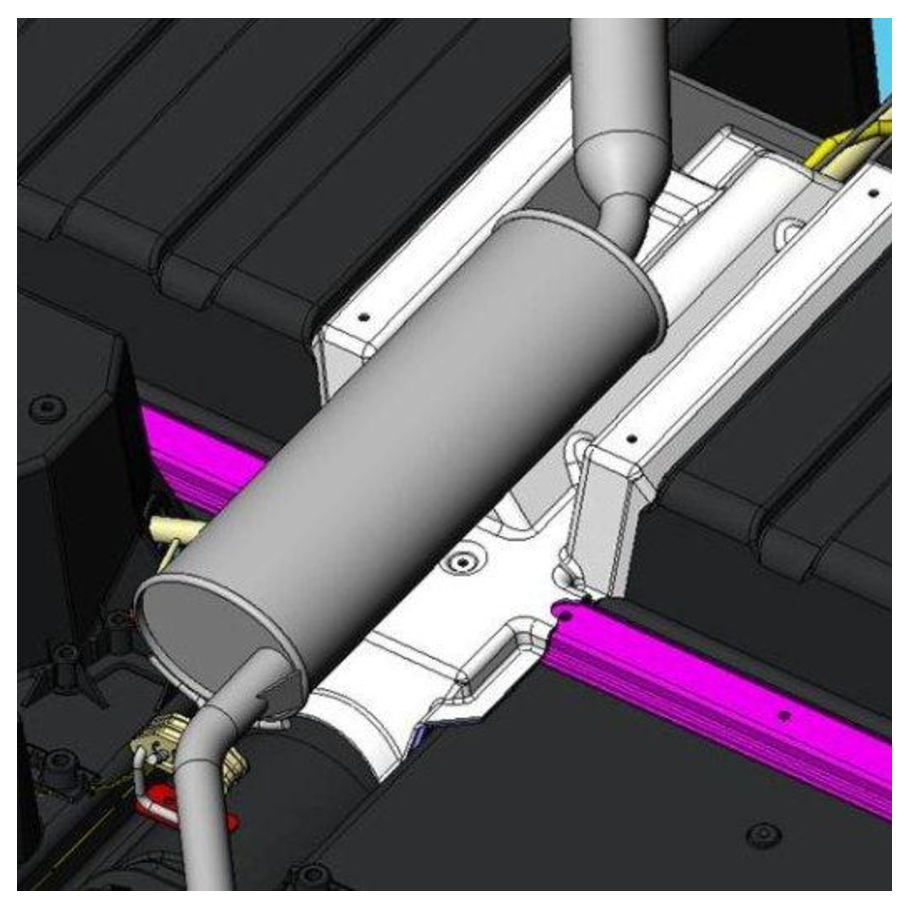
\includegraphics[width=33mm]{AcouSilen0.eps}\hfill
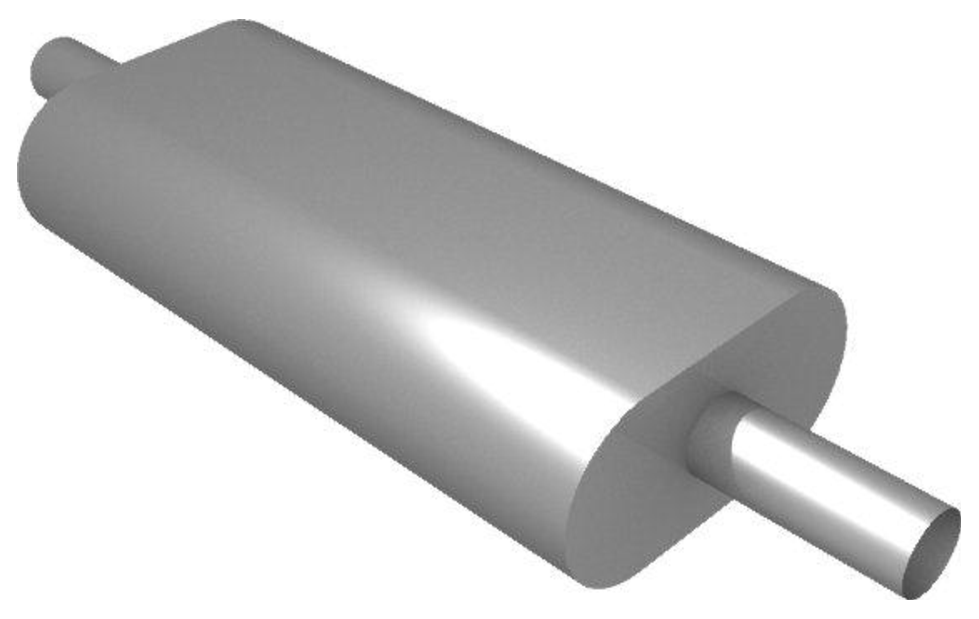
\includegraphics[width=50mm]{AcouSilen1.eps}\hfill
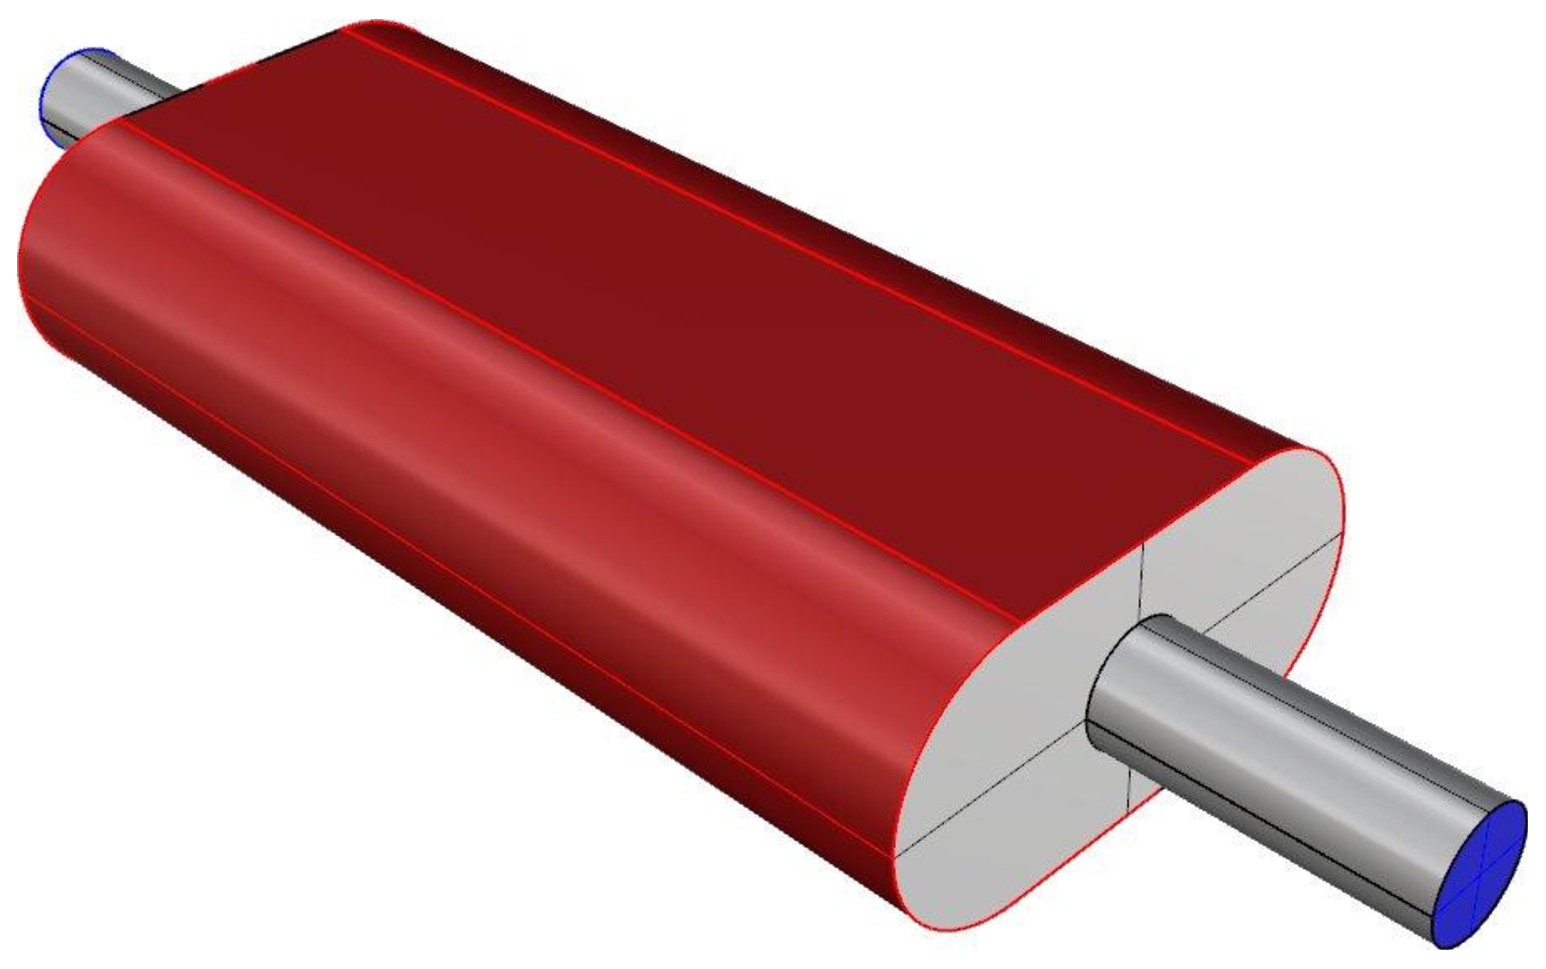
\includegraphics[width=50mm]{AcouSilen2.eps}
\caption{Modélisation d'un silencieux}\label{Fig-AcouSilen}
\end{figure}
Ce silencieux ne sera défini que par les surfaces représentées et le volume d'air qu'elles contiennent. On appliquera aux parois en rouge soit une condition de mur rigide (réflexion parfaite), soit une impédance correspondant à l'absorption due à la présence d'un matériau fibreux (laine de verre). Les surfaces grises seront également considérées comme des surfaces parfaitement réfléchissantes. Les deux section en bleu (on n'en voit qu'une, l'autre étant à l'autre bout) correspondront à l'entrée de l'onde (onde plane) dans le silencieux, et à sa sortie.

On s'intéressera au facteur de perte, tel que défini par la relation~(\ref{Eq-FacPerte}). Les résultats avec et sans absorbant sont illustrés sur la figure~\ref{Fig-AcouSilenRes}, pour des fréquences allant de 25 à 1500~Hz par pas de 25~Hz.
\begin{figure}[h!]
\centering
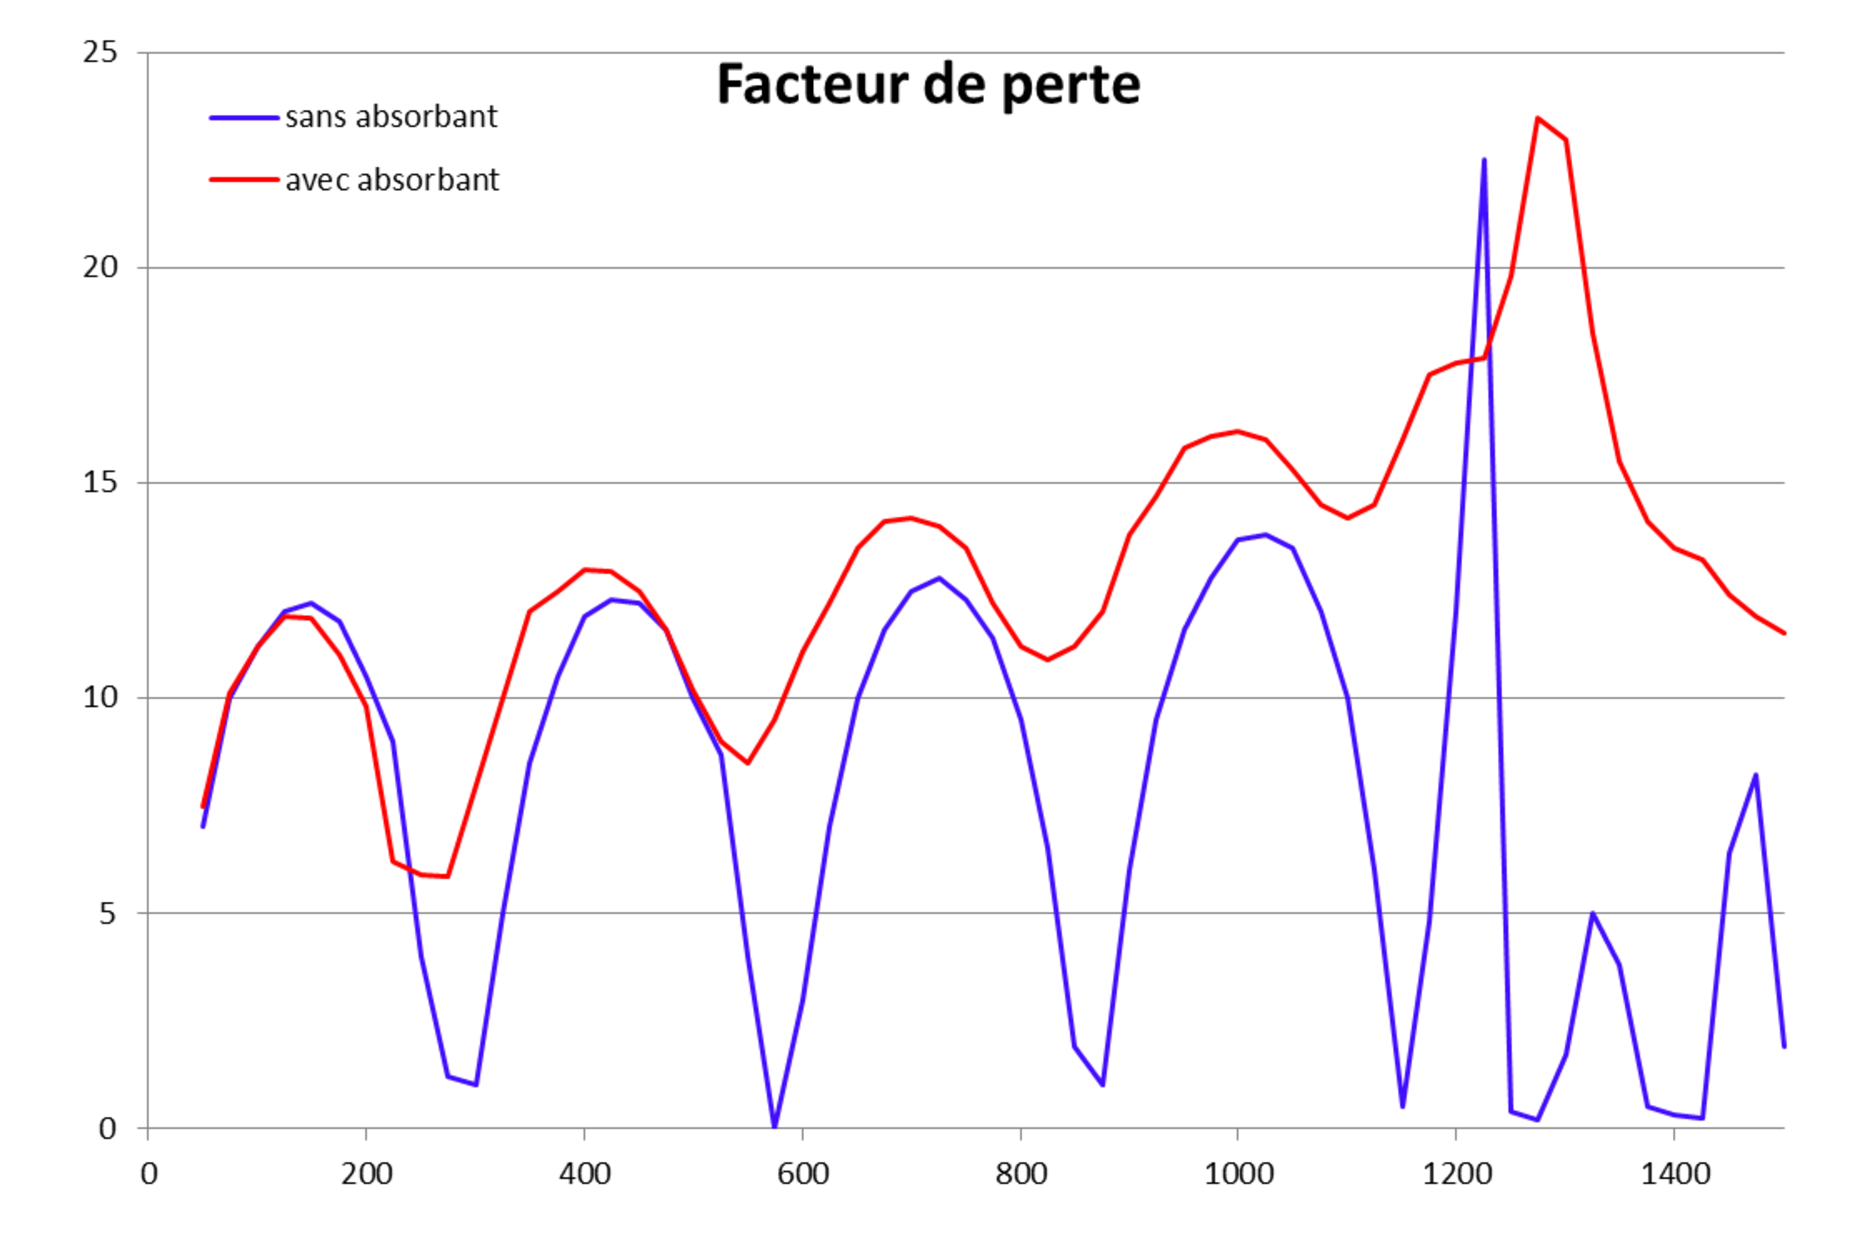
\includegraphics[width=140mm]{AcouSilen3.eps}
\caption{Facteur de perte pour le silencieux}\label{Fig-AcouSilenRes}
\end{figure}
L'influence de l'ajout d'un absorbant est très nette sur ce graphique.

\medskip
\subsection{Deux mots de statistiques}

Nous reprenons ici une remarque faite au paragraphe~\ref{Sec-PInv-Stat}.
Considérons la figure~\ref{Fig-AcouSilenRes}: elle représente la variation d'une réponse~$Y$ (ici le facteur de perte) en fonction d'une entrée~$X$ (ici la fréquence).

Supposons que nous nous intéressions maintenant à ce silencieux sollicité à une fréquence proche de 1000~Hz. On va supposer que la fréquence suit une loi normale centrée sur 1000~Hz et d'écart-type 25~Hz. Évidemment, avec les calculs menés précédemment, nous disposons de peu de points. On va même considérer disposer des points donnés au tableau~\ref{Tab-SilenStat}.
\begin{table}[h!]
\centering
\begin{tabular}{r|ccccc}
Fréquence      & 950  & 975  & 1000 & 1025 & 1050 \\
\hline
Sans absorbant & 11.6 & 12.8 & 13.7 & 13.8 & 13.5 \\
Avec absorbant & 15.8 & 16.1 & 16.2 & 16.0 & 15.3\\
poids $1000.p_i$& 2.16 & 9.68 & 15.96 & 9.68 & 2.16
\end{tabular}
\caption{Points disponibles pour l'approximation de la moyenne}\label{Tab-SilenStat}
\end{table}
L'application de la formule~(\ref{Eq-PInv-Stat}) sur ces quelques points conduit à une première approximation de la moyenne du facteur de perte de~$13.38$ sans absorbant et~$16.06$ avec absorbant.

Évidemment, c'est une première approximation très grossière, qui peut être améliorée. Pour cela, il nous faudrait disposer de plus de points, aussi bien dans le domaine considéré qu'en dehors. Si l'on ne peut relancer de calcul, on peut essayer d'approximer la courbe de la réponse afin de pouvoir interpoler et extrapoler des points.

On peut utiliser tout type d'interpolation (voir chapitre~\ref{chap-interpolation}) comme par exemple un polynôme de Lagrange... ici nous utiliserons une courbe de tendance polynomiale de degré 2. Dans le cas sans absorbant, celle-ci est donnée par l'équation suivante: $y= -0,0004342857x^2 + 0,8877714286x - 439,8628571429$. De là, on peut générer quelques points supplémentaires. Vu la forme de la courbe de réponse, on sait que les valeurs interpolées seront correctes, ce n'est pas le cas pour les valeurs extrapolées, surtout loin de la zone ayant servie à générer cette courbe de tendance. Par exemple on trouve 12.6 pour 1075~Hz au lieu de 12.0, 11.2 pour 1100~Hz au lieu de 10.0. Néanmoins, en fonction de la forme de la courbe, cela peut permettre une amélioration sensible de l'approximation de la moyenne de la réponse.

Pour une analyse plus complète dans le cadre stochastique, c'est au chapitre~\ref{Ch-stocha} que l'on se reportera. Toutes les méthodes décrites sont applicables en fréquence.


\medskip
\subsection{Sur les conditions aux limites}

\begin{wrapfigure}{l}{65mm}
\centering
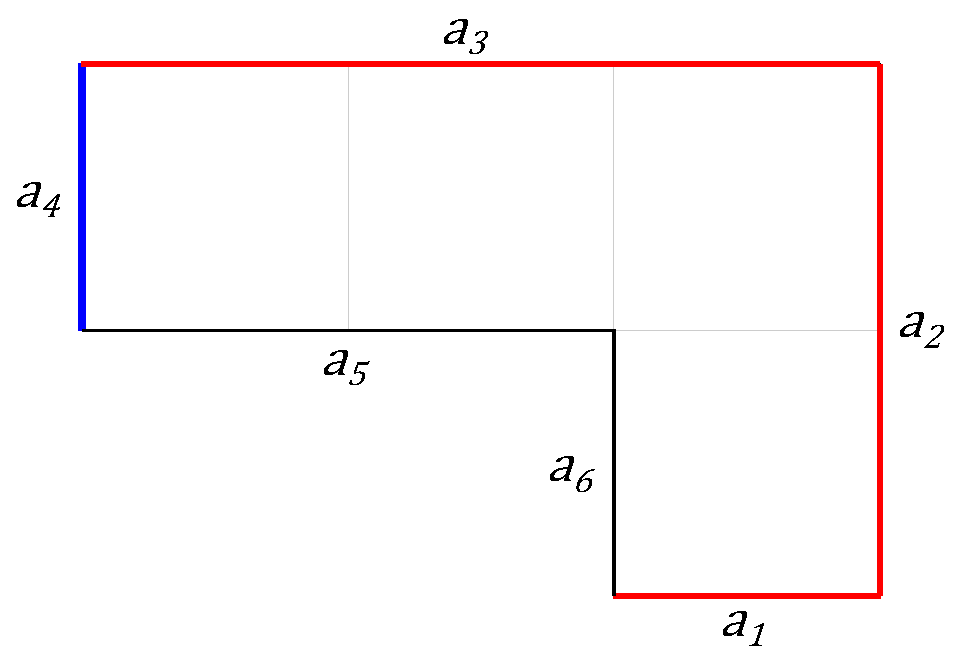
\includegraphics[width=55mm]{AcouDiff0.eps}
\caption{Acoustique et obstacle}\label{Fig-AcouDiff0}
\end{wrapfigure}
Nous nous proposons de retrouver l'illustration~\ref{Fig-diffrac}d.

Pour cela, nous considérons le modèle décrit à la figure~\ref{Fig-AcouDiff0} constitué de 6 segments~$a_1$ à $a_6$. L'onde acoustique incidente arrive par le segment~$a4$. L'onde est libre de se propager, et notamment elle n'est pas réfléchie sur les côtés~$a_1$ à~$a_3$, l'obstacle ne correspondant qu'aux faces~$a_5$ et~$a_6$.

Pour modéliser l'onde arrivant dans le modèle, on va supposer que la surface~$a_4$ porte une condition de Dirichlet de type~$p=\overline{p}$.
Nous proposons, dans un premier temps, d'imposer sur les faces~$a_1$ à~$a_3$ une condition de Dirichlet de type~$p=0$.
Nous utiliserons \freefem pour cet exemple.

Dans un premier temps, nous allons entrer directement la formulation faible définie à l'aide des formes bilinéaire~(\ref{Eq-Helmacomplex}) et linéaire~(\ref{Eq-Helmacomplex}) que nous rappelons:
\begin{equation}
a(p,q)=\dint_\Omega \partial_{x_i}p\partial_{x_i}\tilde{q}-k^2p\tilde{q} +
\dint_{\Gamma_R} i\rho ckA_n\tilde{q}
\quad \text{ et } \quad
b(q)=-\dint_{\Gamma_N} i\rho c k\overline{V}_n q
\end{equation}

\medskip
La description de la géométrie et le maillage sont donnés par:
\colorgris\scriptsize
\begin{Verbatim}[numbers=left,numbersep=3pt]
real freq=200;// fréquence en Hz
real c=343;// vitesse du son en m/s
func g=1;// on a p=g sur a4 => onde plane, par condition de Dirichlet
real k=freq/c;

border a1(t=0,1) { x= 2+t; y=0;}
border a2(t=0,1) { x=3; y= 2*t;}
border a3(t=0,1) { x= 3-3*t; y=2 ;}
border a4(t=0,1) { x= 0; y= 2-t ;}
border a5(t=0,1) { x= 2*t; y= 1 ;}
border a6(t=0,1) { x= 2; y=1-t ;}

mesh Th=buildmesh( a1(20) + a2(40) + a3(60) + a4(20) + a5(40) + a6(20));
\end{Verbatim}
\colorblack\normalsize

\medskip
Écrivons maintenant brutalement notre formulation faible:
\colorgris\scriptsize
\begin{Verbatim}[numbers=left,numbersep=3pt,firstnumber=last]
fespace Vh(Th, P2);
Vh<complex> p, q;

solve helmholtz(p,q)= int2d(Th)(dx(p)*dx(conj(q)) + dy(p)*dy(conj(q)) - k*k*p*conj(q) )
 -int1d(Th,a4)(g*q) + on(a1,p=0) + on(a2,p=0)+ on(a3,p=0);
plot (p, wait=1, ps="AcouDiff3.eps");
\end{Verbatim}
\colorblack\normalsize

\medskip
Le résultat est donné à la figure~\ref{Fig-AcouDiff3} pour plusieurs valeurs de la fréquence.
\begin{figure}[h!]
\centering
\ifVersionDuDocEstVincent
   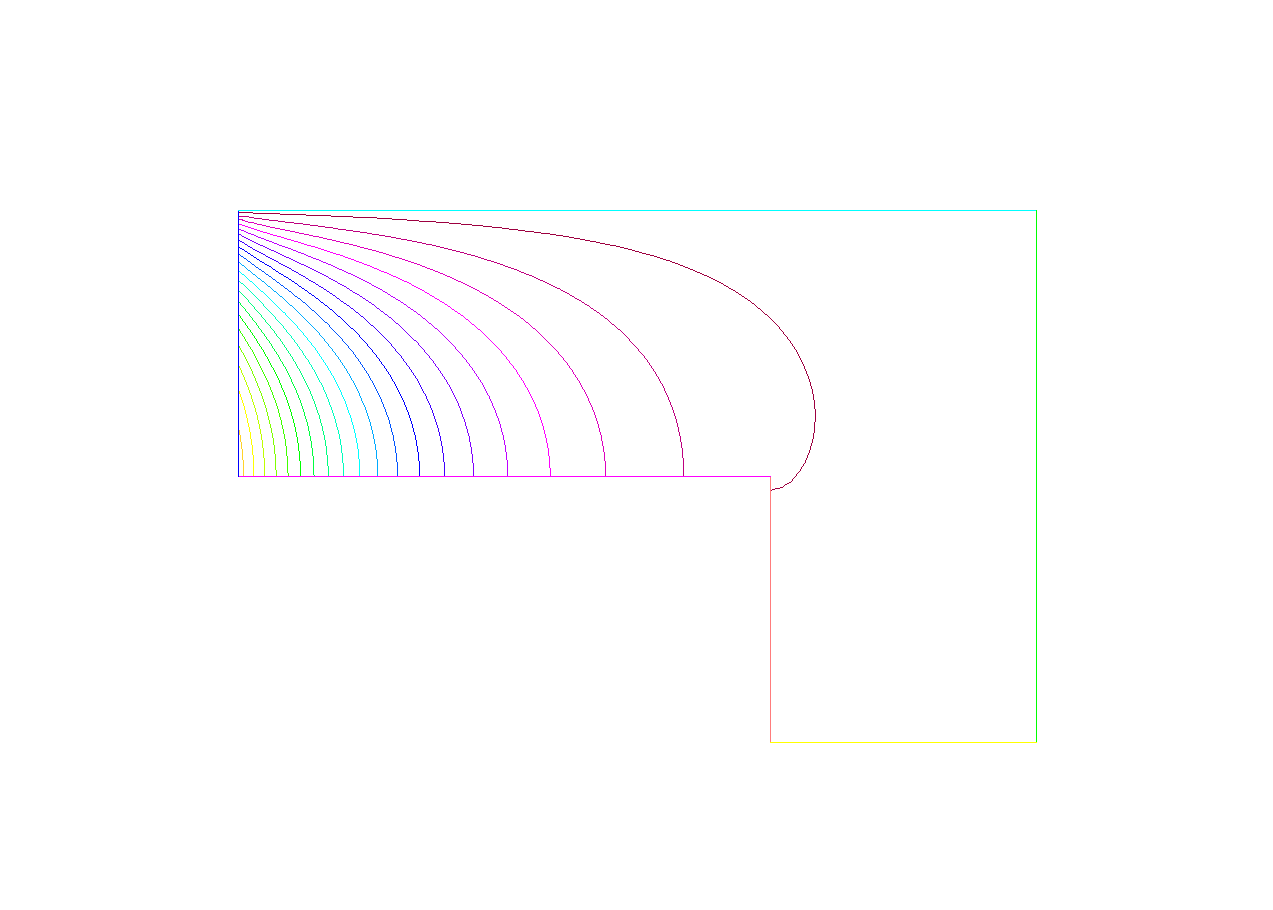
\includegraphics[width=57mm]{AcouDiff1-1.eps}\hfill
   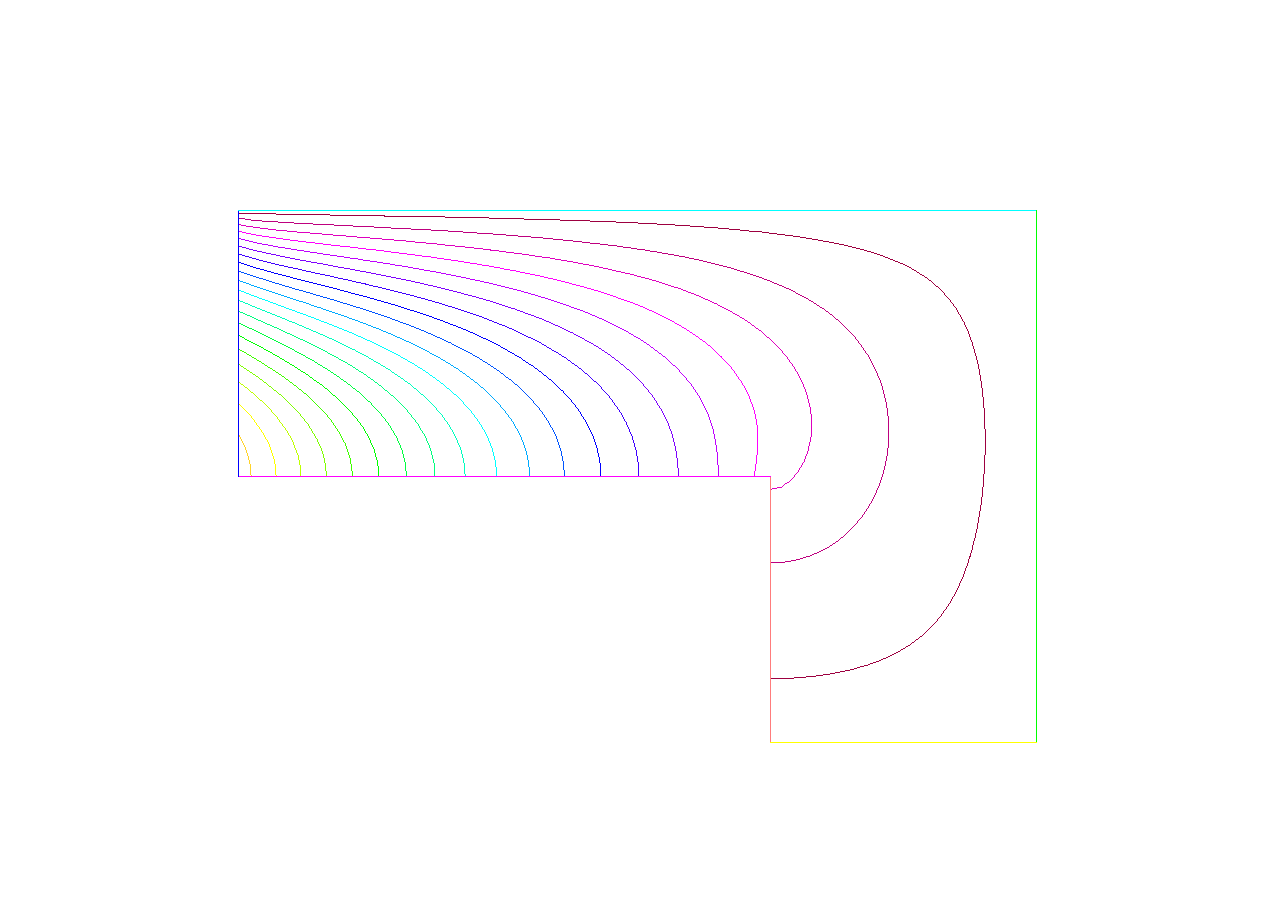
\includegraphics[width=57mm]{AcouDiff1-5.eps}\hfill
   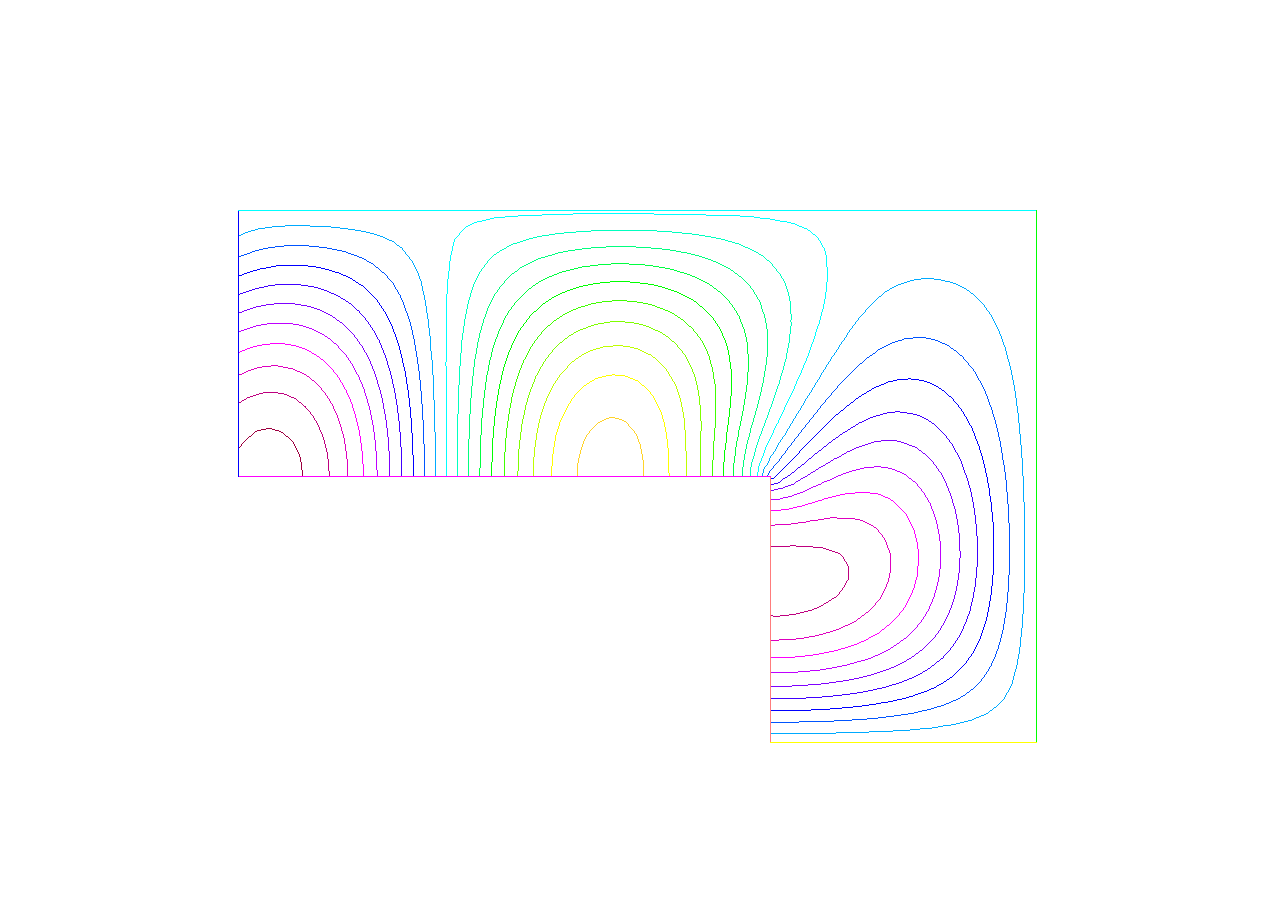
\includegraphics[width=57mm]{AcouDiff1-10.eps}
\else
   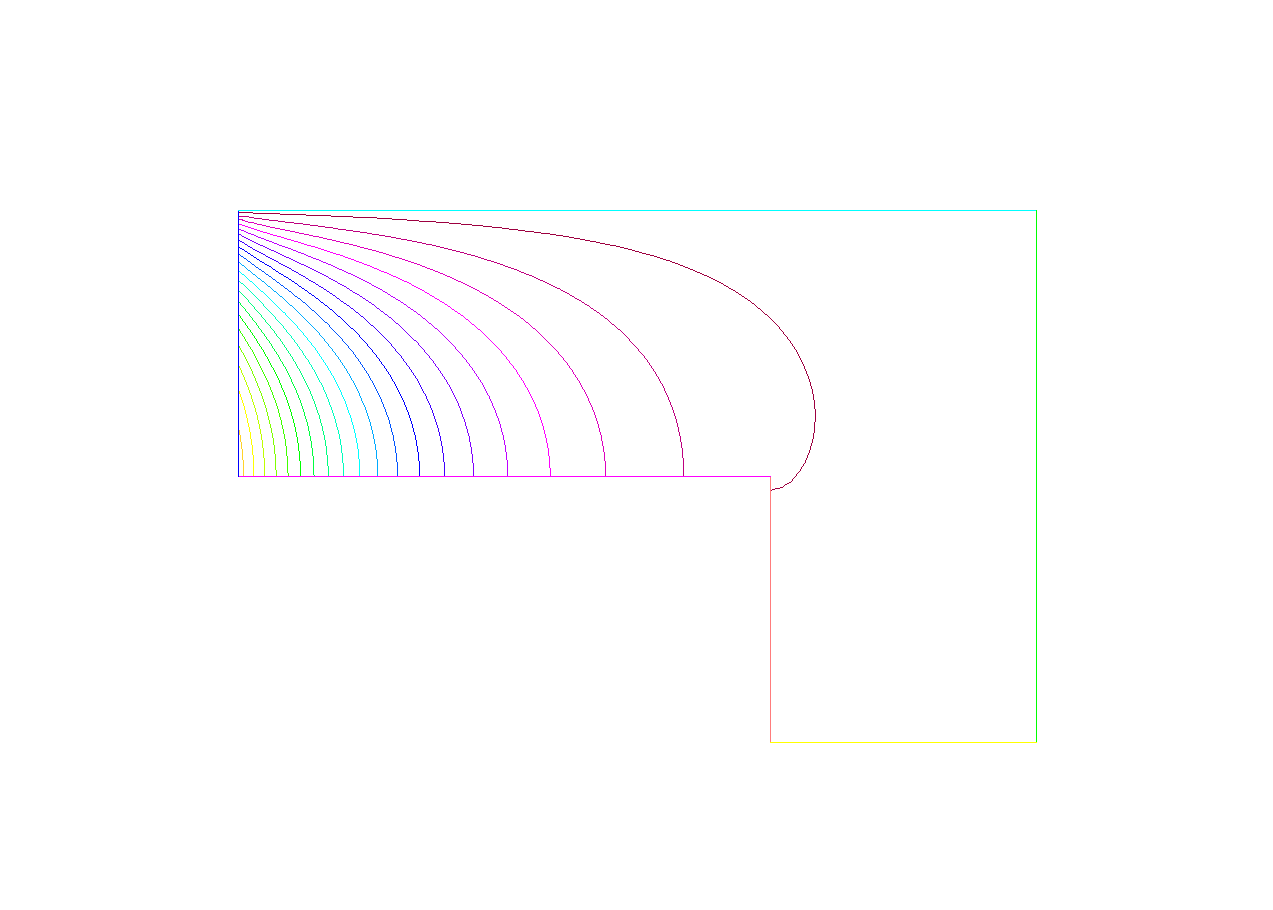
\includegraphics[width=50mm]{AcouDiff1-1.eps}\hfill
   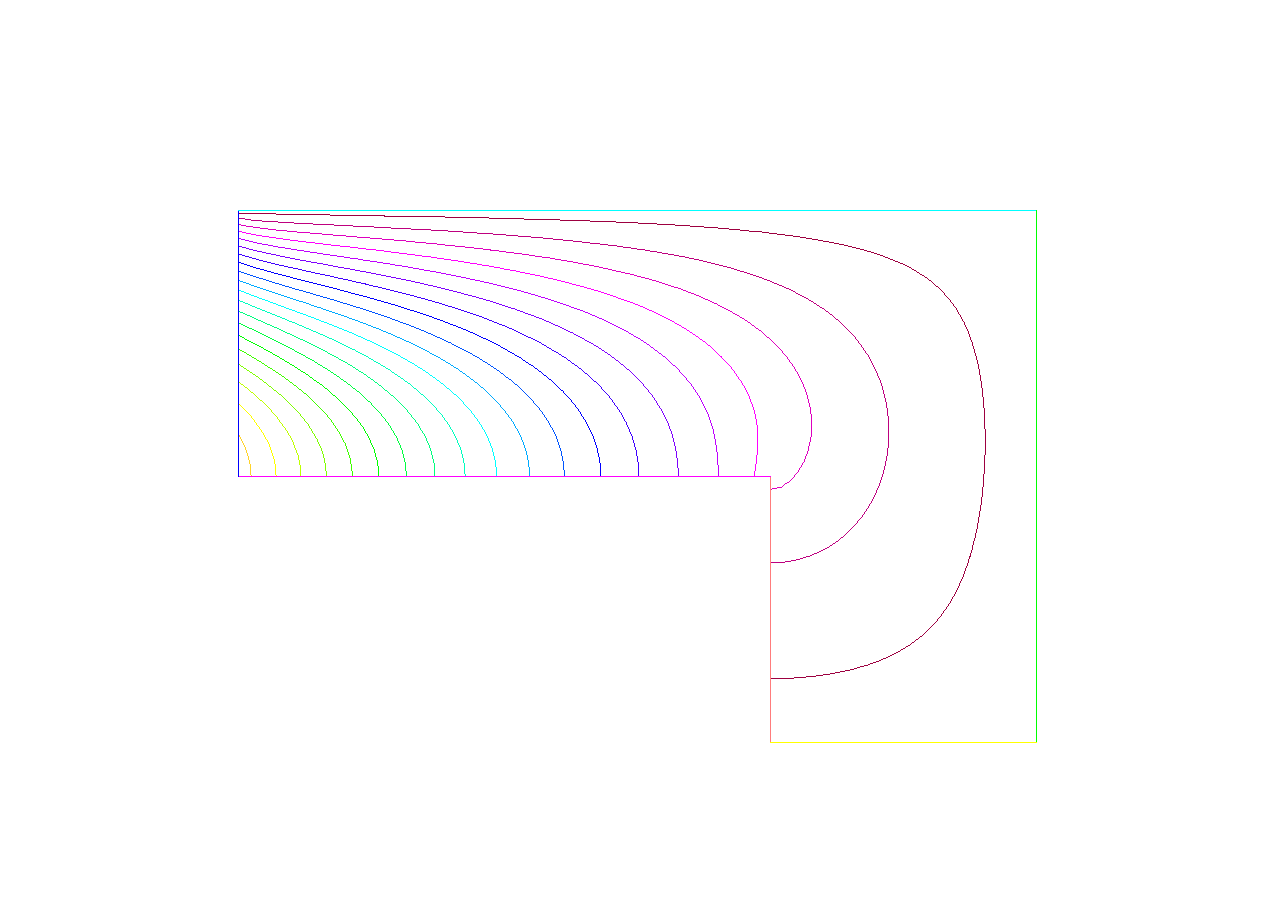
\includegraphics[width=50mm]{AcouDiff1-5.eps}\hfill
   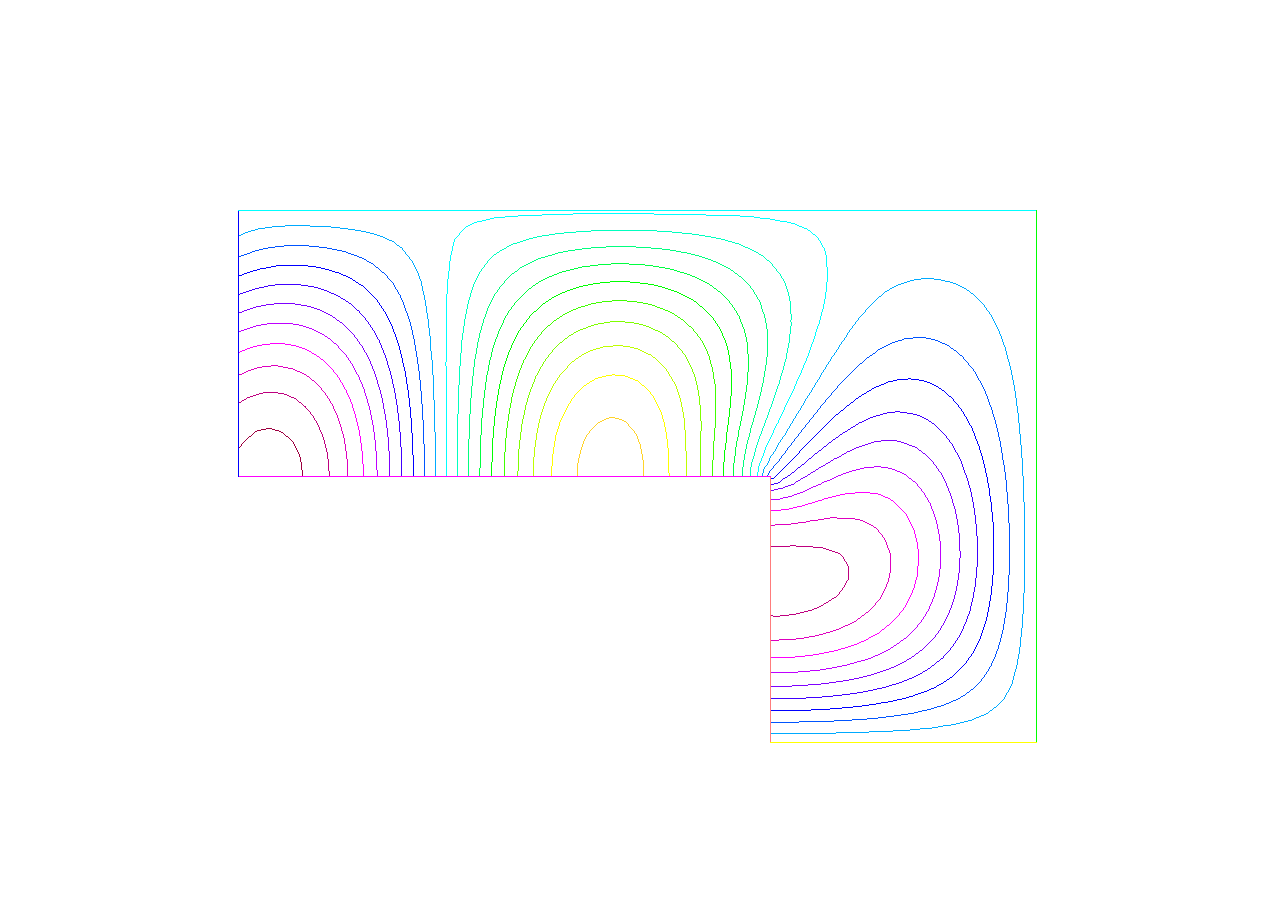
\includegraphics[width=50mm]{AcouDiff1-10.eps}
\fi
\caption{Acoustique au coin de la rue pour des fréquences de~$100$, $500$ et $1000$~Hz}\label{Fig-AcouDiff3}
\end{figure}

\medskip\noindent
Y a-t-il un intérêt à demander une approximation P2?
\flushright
\textcolorgris{\reflectbox{Yaka essayer... ici non. Valeurs quasiment identiques.}}
\flushleft

Les conditions aux limites sont-elles satisfaisantes?
\flushright
\colorgris{\reflectbox{Pas vraiment!}\\ 
\reflectbox{Imposer~$p=0$ ne correspond pas à une condition aux limites de type «fuite» à l'infini.}\\
\reflectbox{On force seulement la pression à être nulle au bord, d'où la forme de la répartition...}\colorblack\flushleft

\medskip
Modifions le script précédent, et ne passons pas en complexes:
\colorgris\scriptsize
\begin{Verbatim}[numbers=left,numbersep=3pt,firstnumber=14]
fespace Vh(Th,P1);
Vh p,q;

 solve helmholtz(p,q)= int2d(Th)(dx(p)*dx(q) + dy(p)*dy(q) - k*k*p*q )
 -int1d(Th,a4)(g*q) + on(a1,p=0) + on(a2,p=0)+ on(a3,p=0);

string legende="frequence = "+freq+" Hz";
plot (p, wait=true, cmm=legende, fill=1, value=true);
\end{Verbatim}
\colorblack\normalsize

\medskip\noindent
Y a-t-il une différence?
\flushright
\textcolorgris{\reflectbox{Yaka essayer... ici non. Valeurs quasiment identiques.}}
\flushleft

\medskip
Et si on entrait une condition de Neumann? Là, il est nécessaire d'être en complexe. L'unité complexe sous \freefem est \verb|1i|.
\colorgris\scriptsize
\begin{Verbatim}[numbers=left,numbersep=3pt,firstnumber=14]
fespace Vh(Th, P2);
Vh<complex> p, q;

solve helmholtz(p,q)= int2d(Th)(p*q*k*k - dx(p)*dx(q) - dy(p)*dy(q))
 -int1d(Th,a4)(g*q) -int1d(Th,a1)(1i*c*k*q)-int1d(Th,a2)(1i*c*k*q)-int1d(Th,a3)(1i*c*k*q);

string legende="frequence = "+freq+" Hz";
plot (p, wait=true, cmm=legende, fill=1, value=true);
\end{Verbatim}
\colorblack\normalsize

\medskip
Cette fois la réponse est nécessairement différente, puisque les conditions aux limites ne sont pas les mêmes... les résultats correspondants sont à la figure~\ref{Fig-AcouDiff2}.
\begin{figure}[h!]
\centering
\ifVersionDuDocEstVincent
   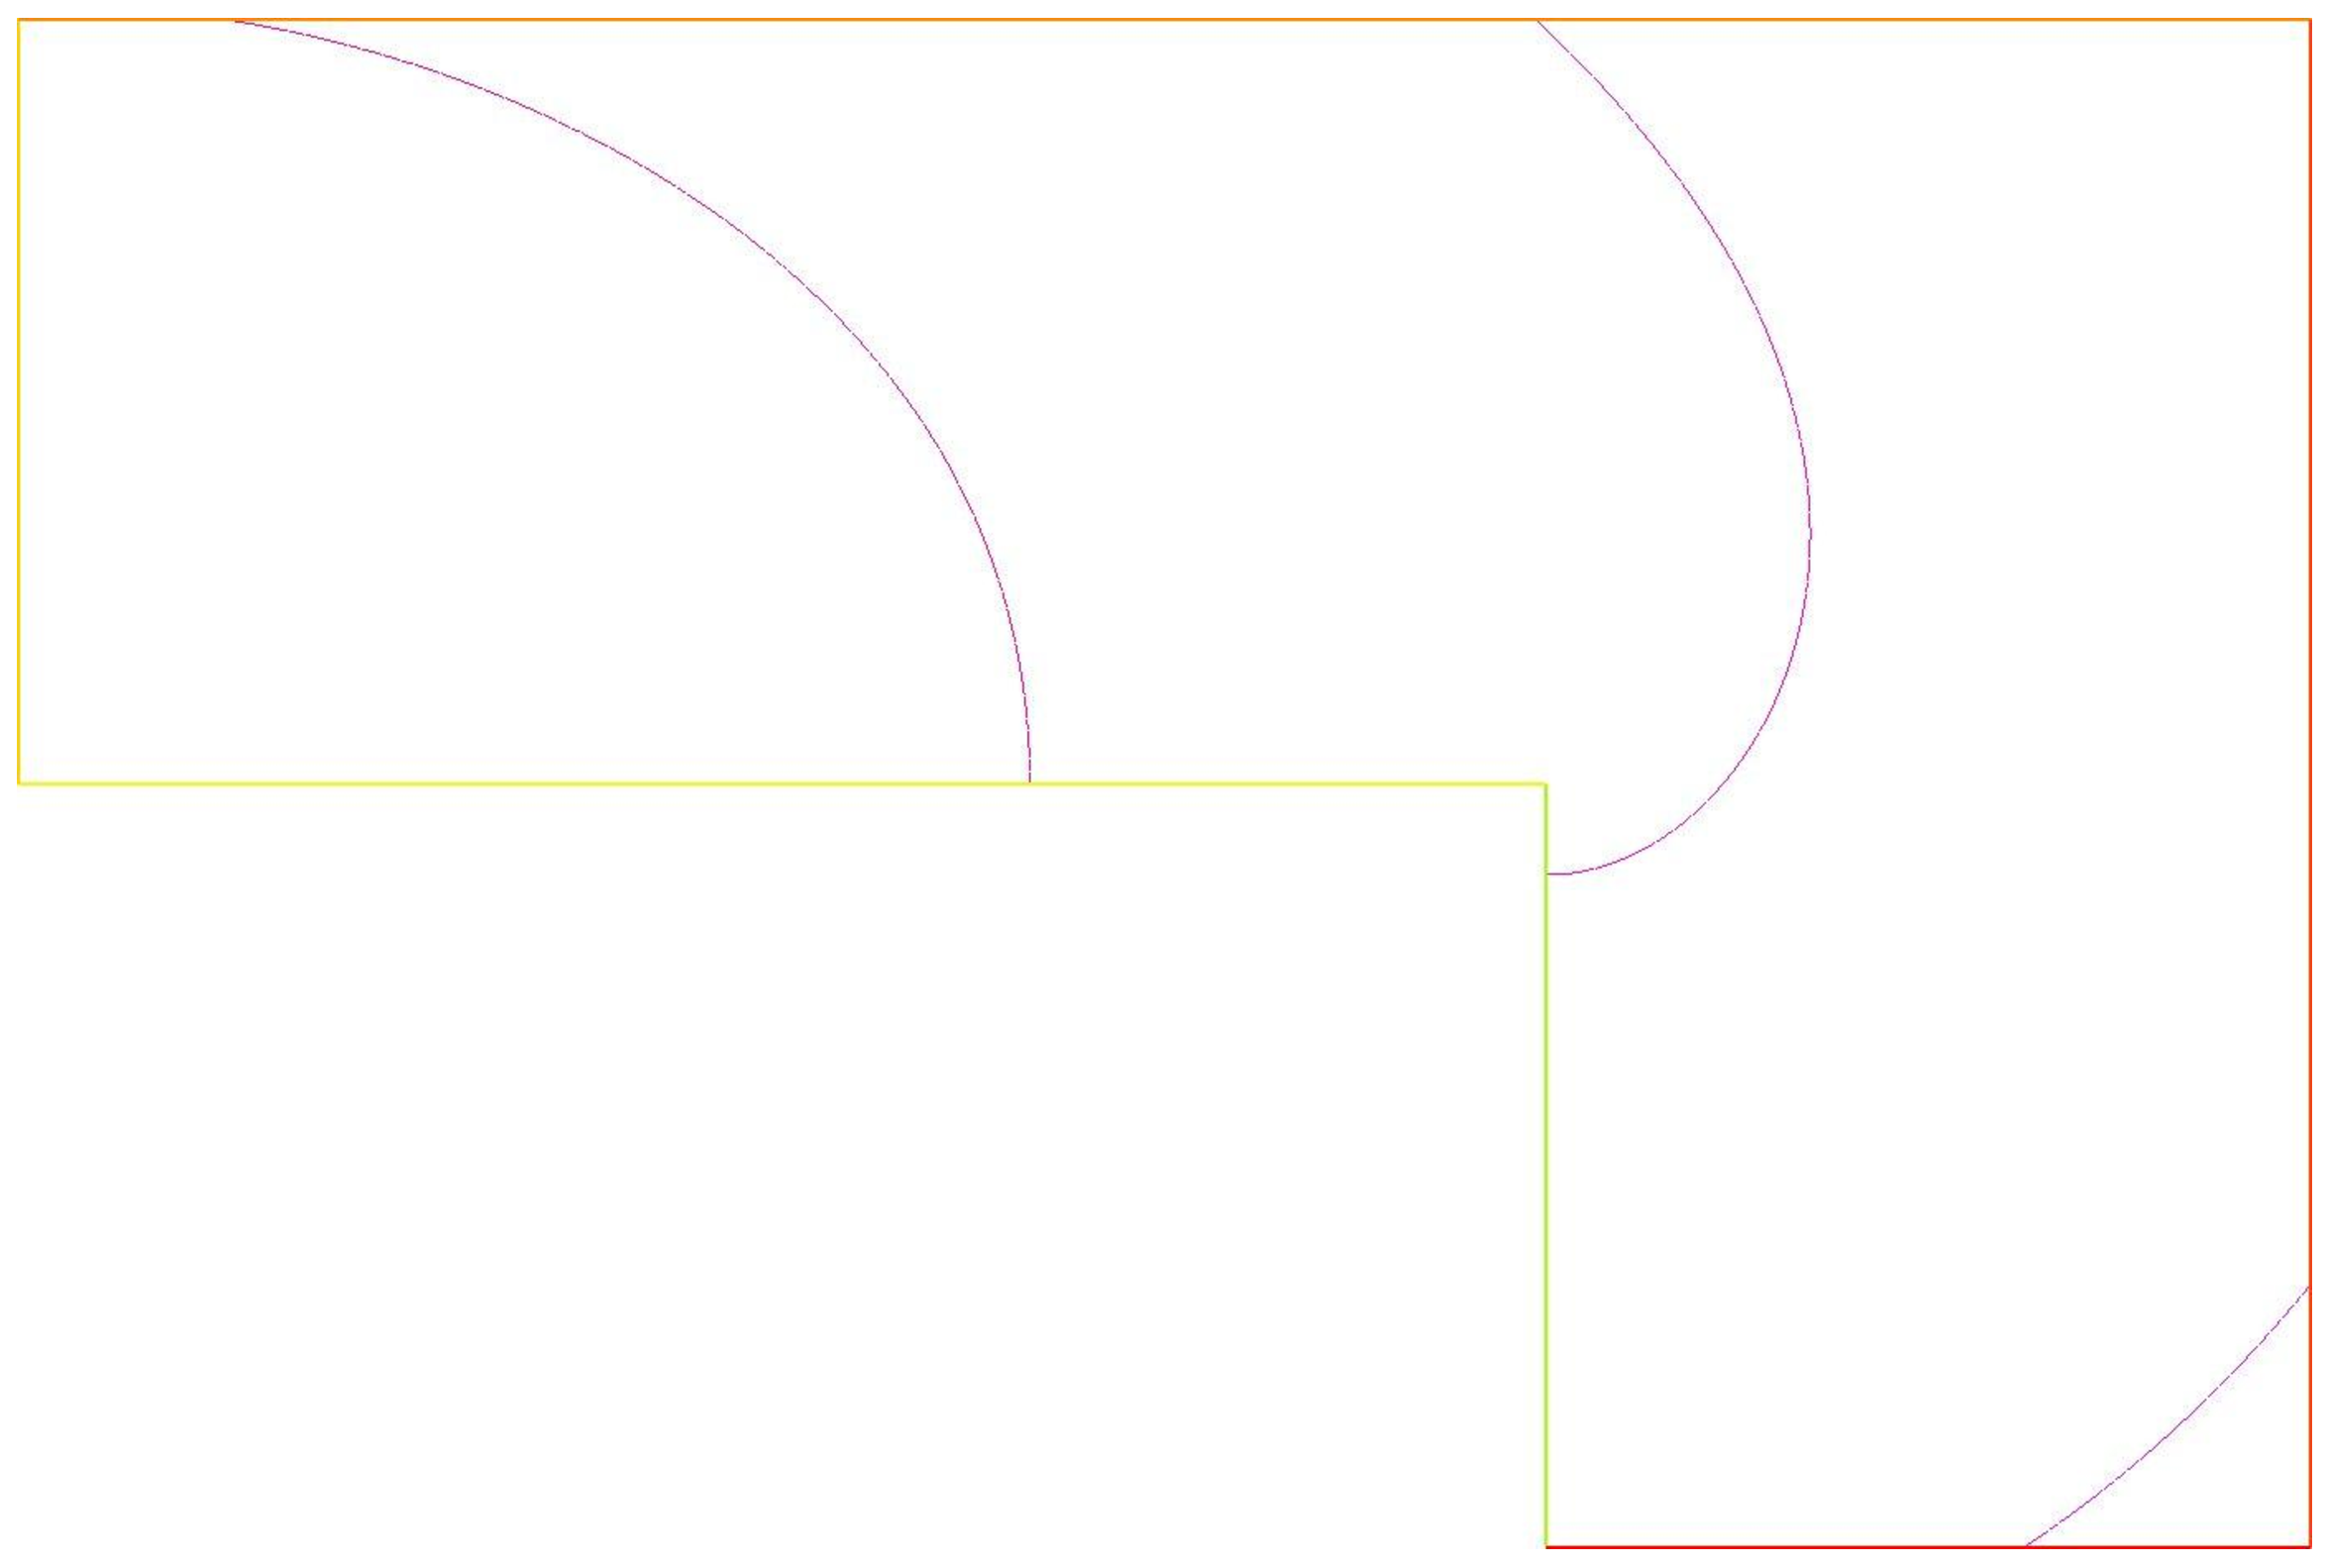
\includegraphics[width=40mm]{AcouDiff2-1.eps}\hfill
   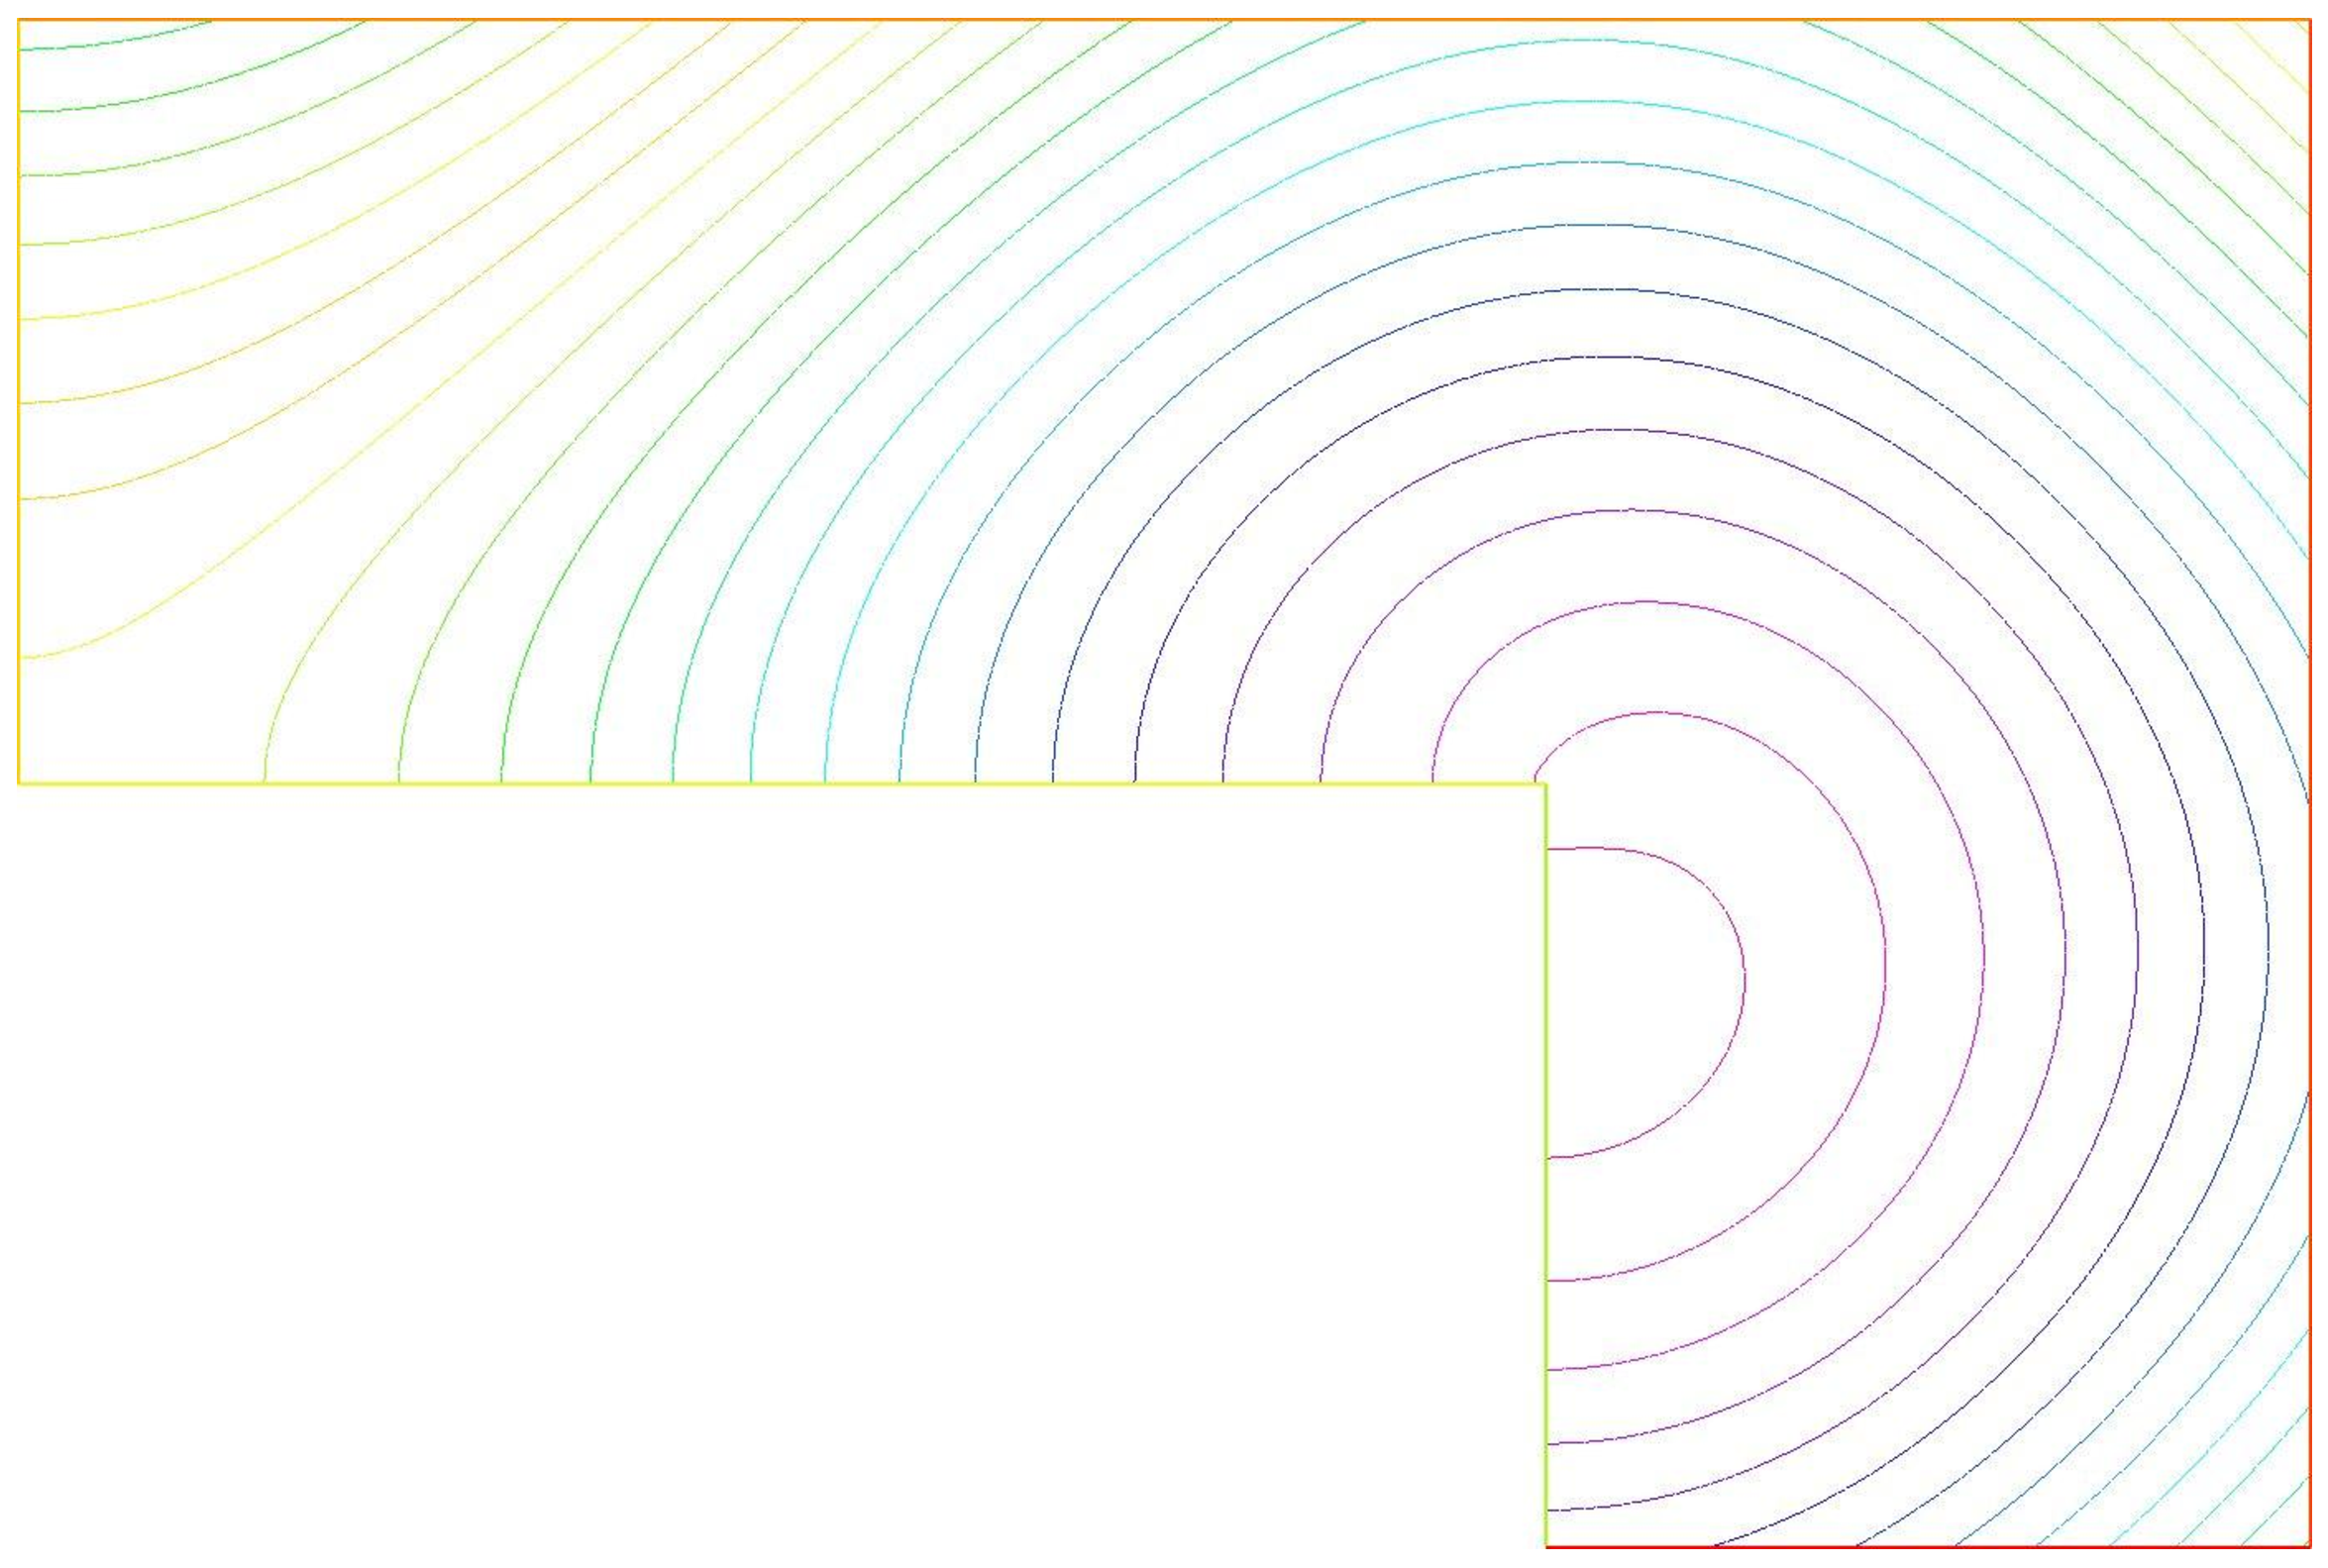
\includegraphics[width=40mm]{AcouDiff2-5.eps}\hfill
   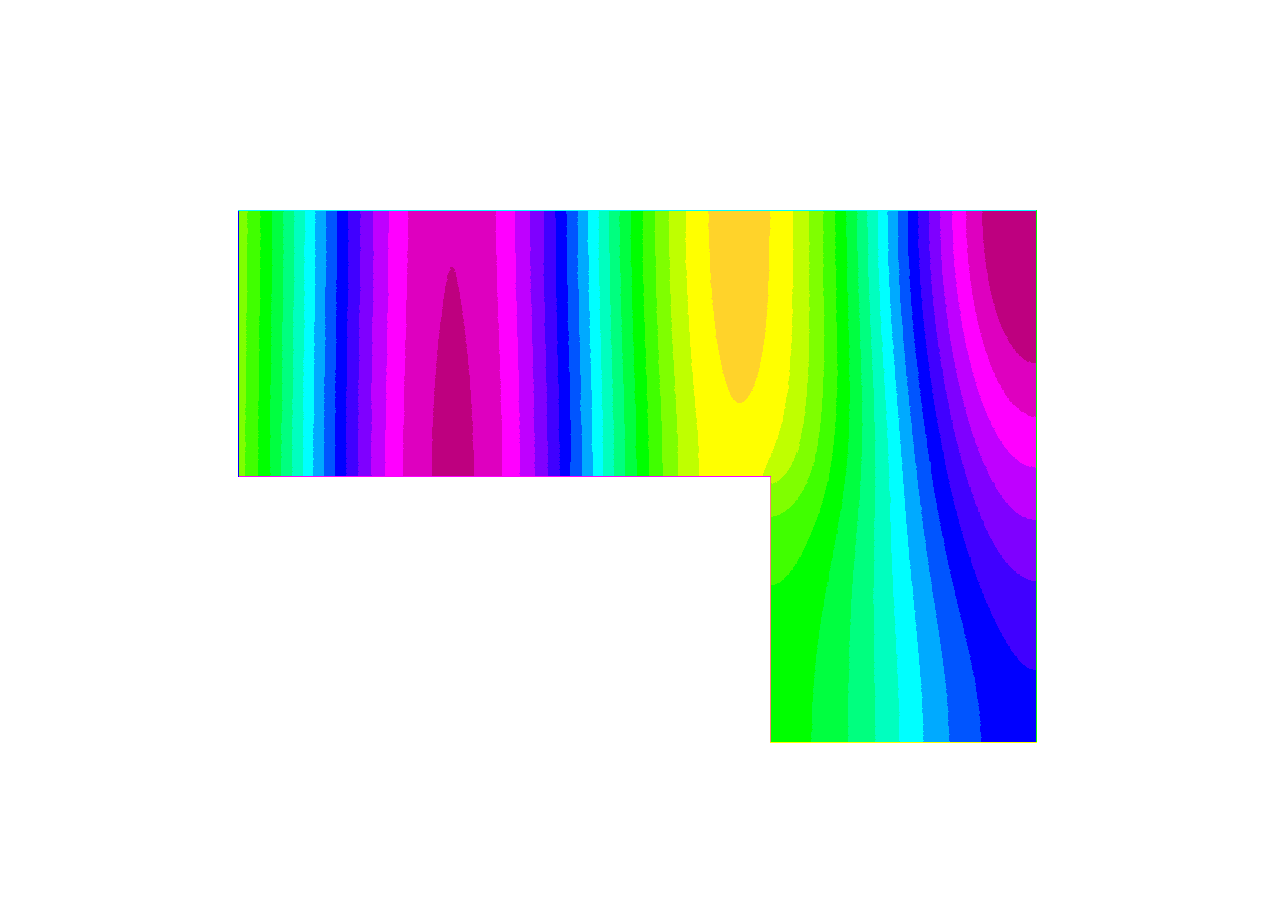
\includegraphics[width=40mm]{AcouDiff2-10.eps}
\else
   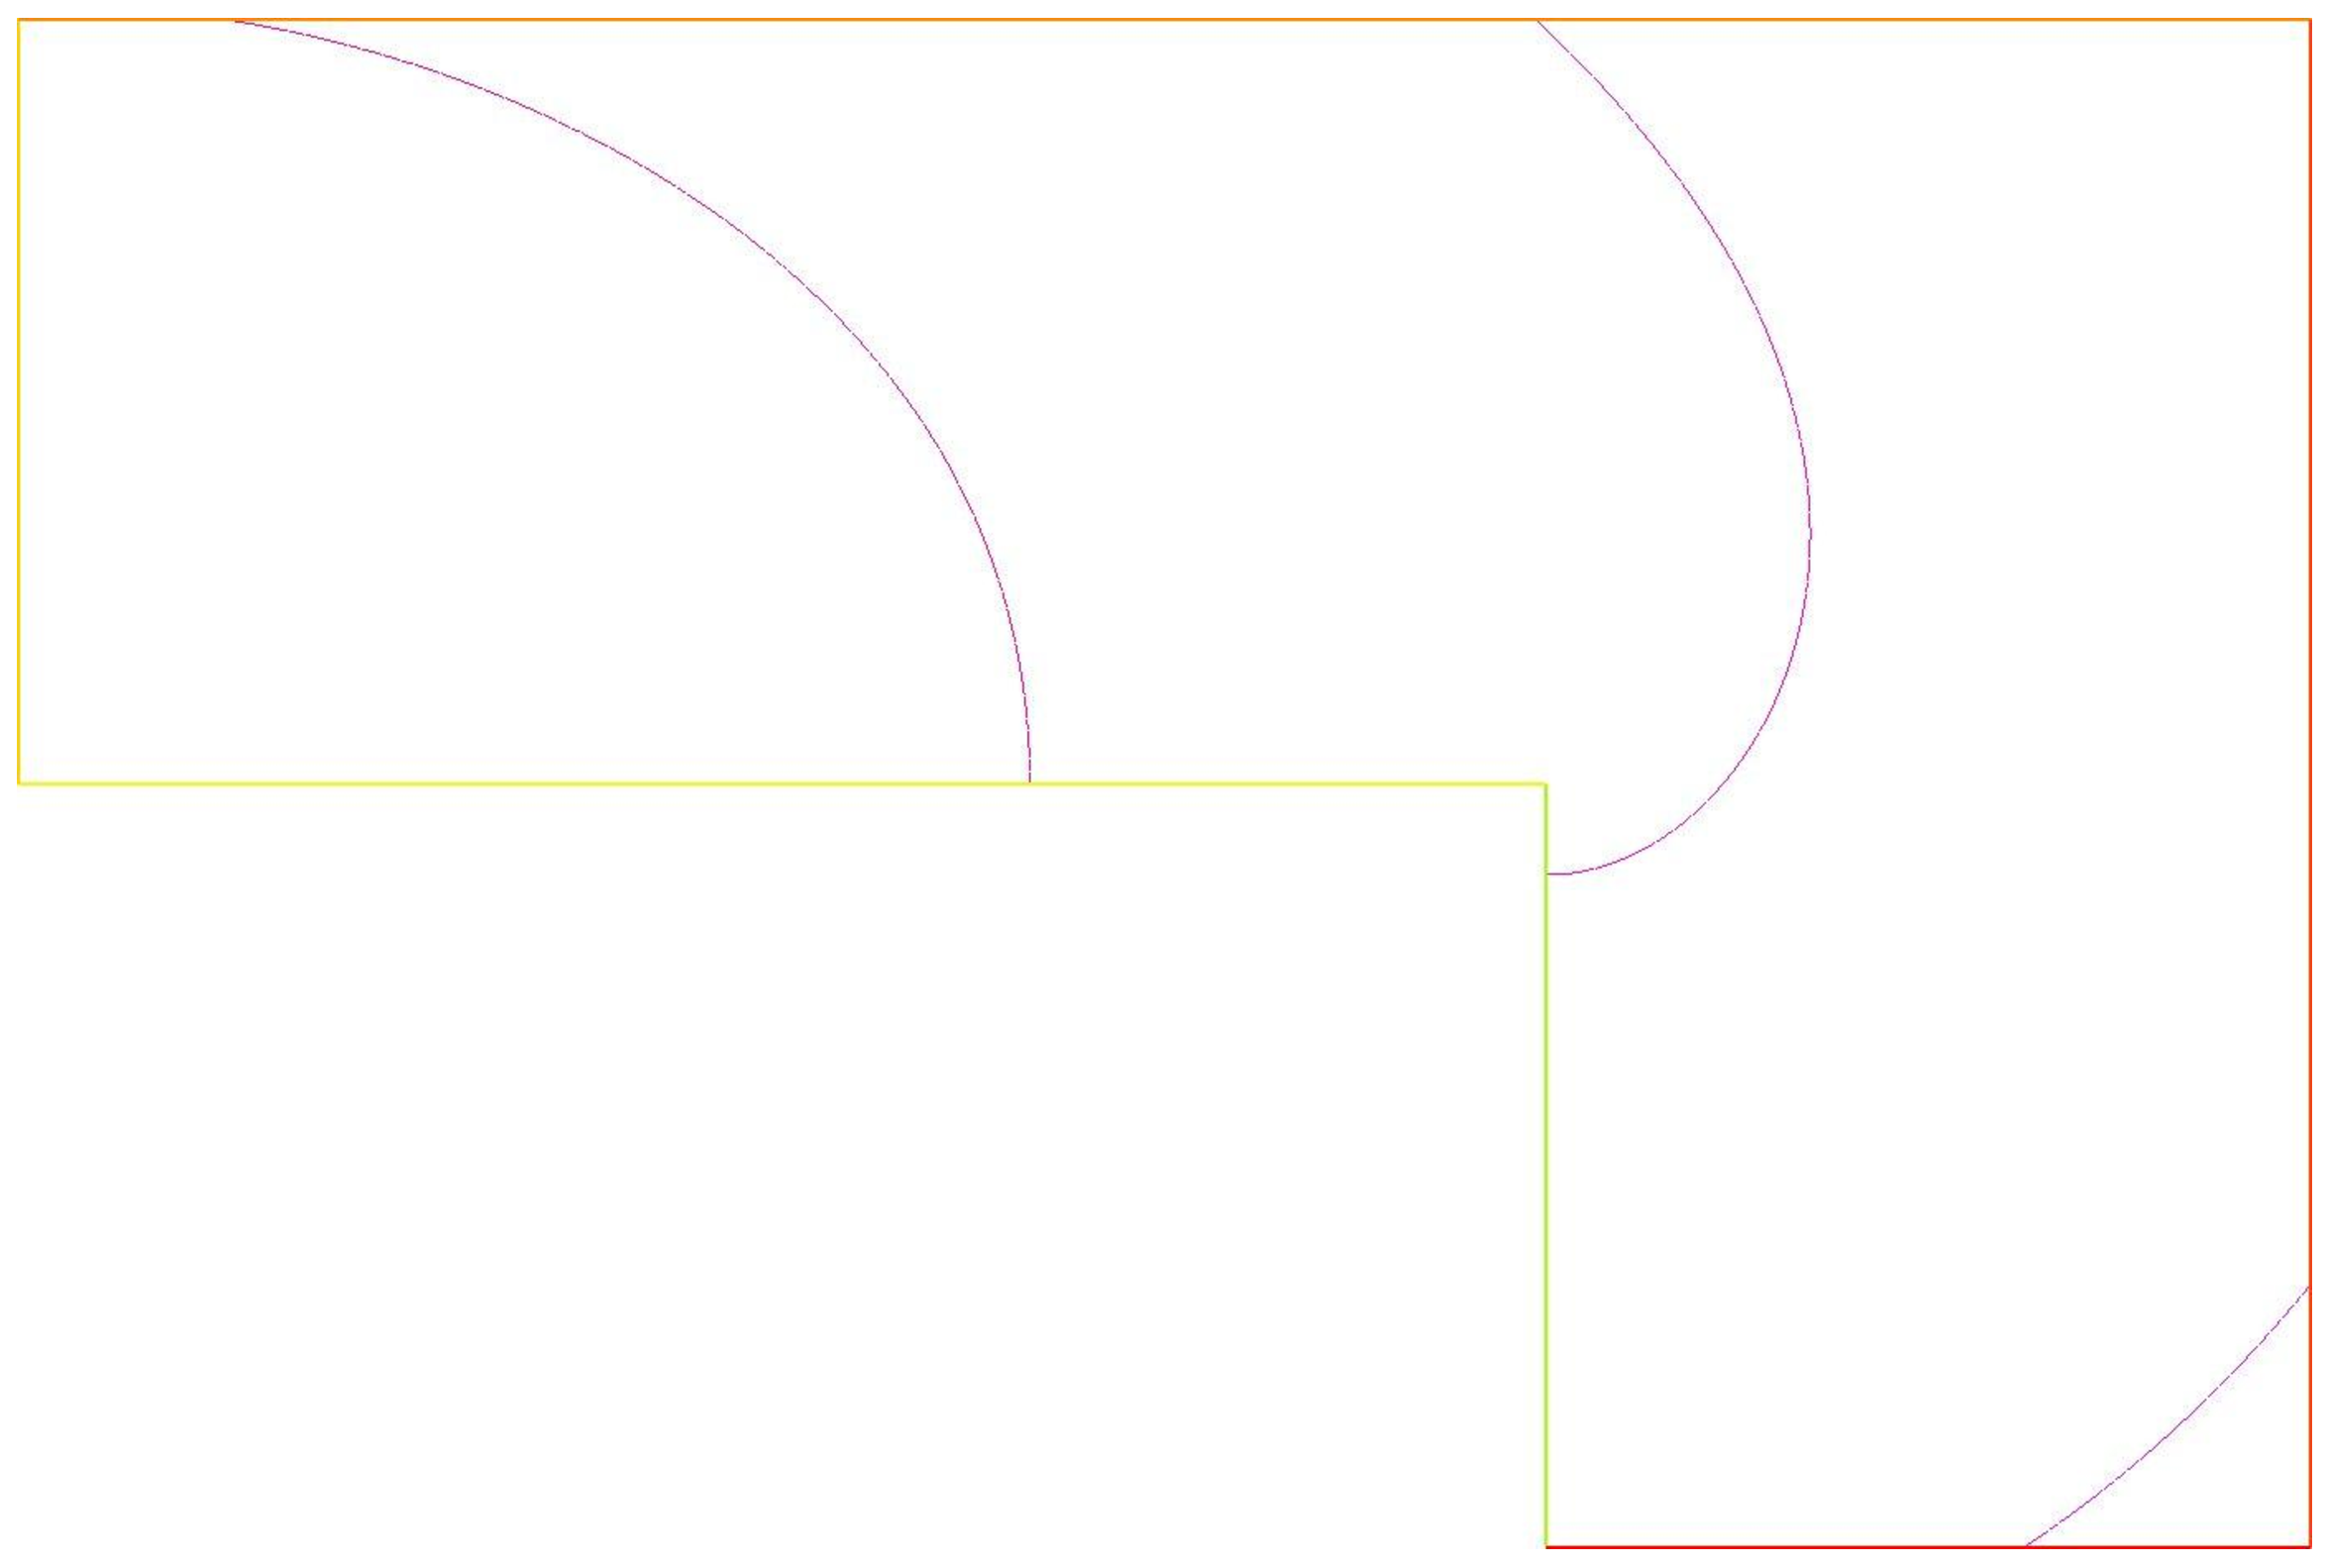
\includegraphics[width=33mm]{AcouDiff2-1.eps}\hfill
   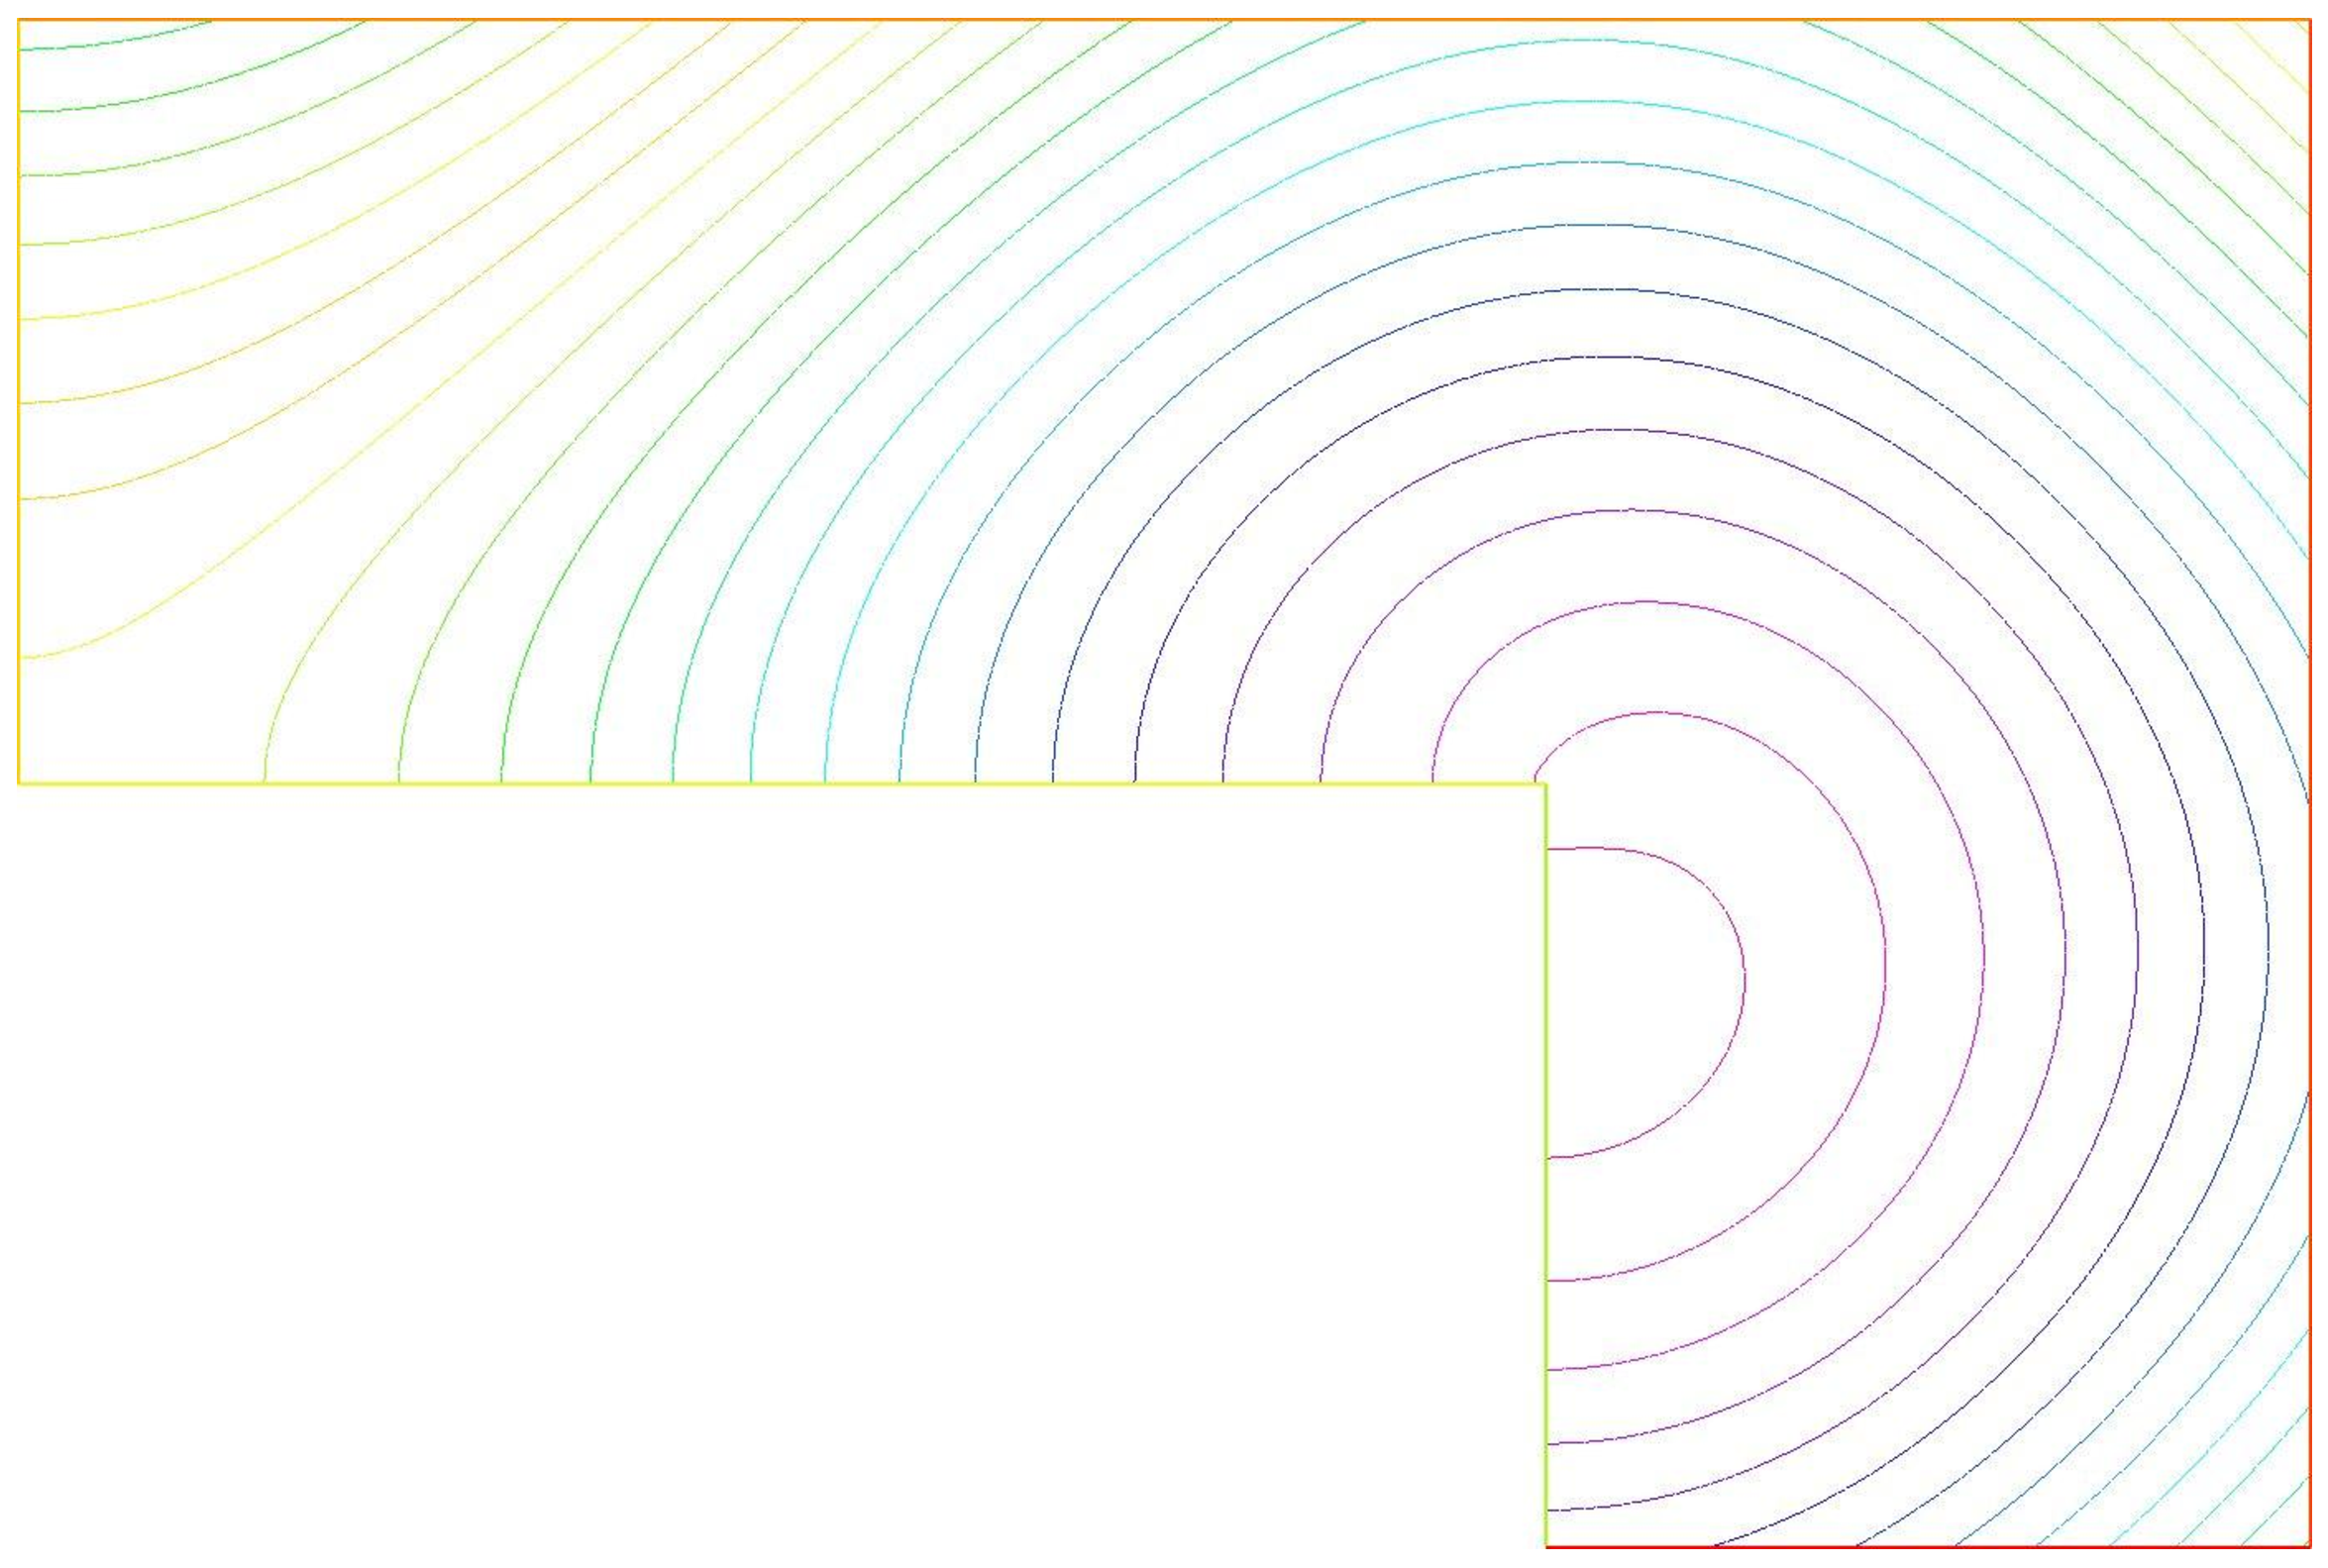
\includegraphics[width=33mm]{AcouDiff2-5.eps}\hfill
   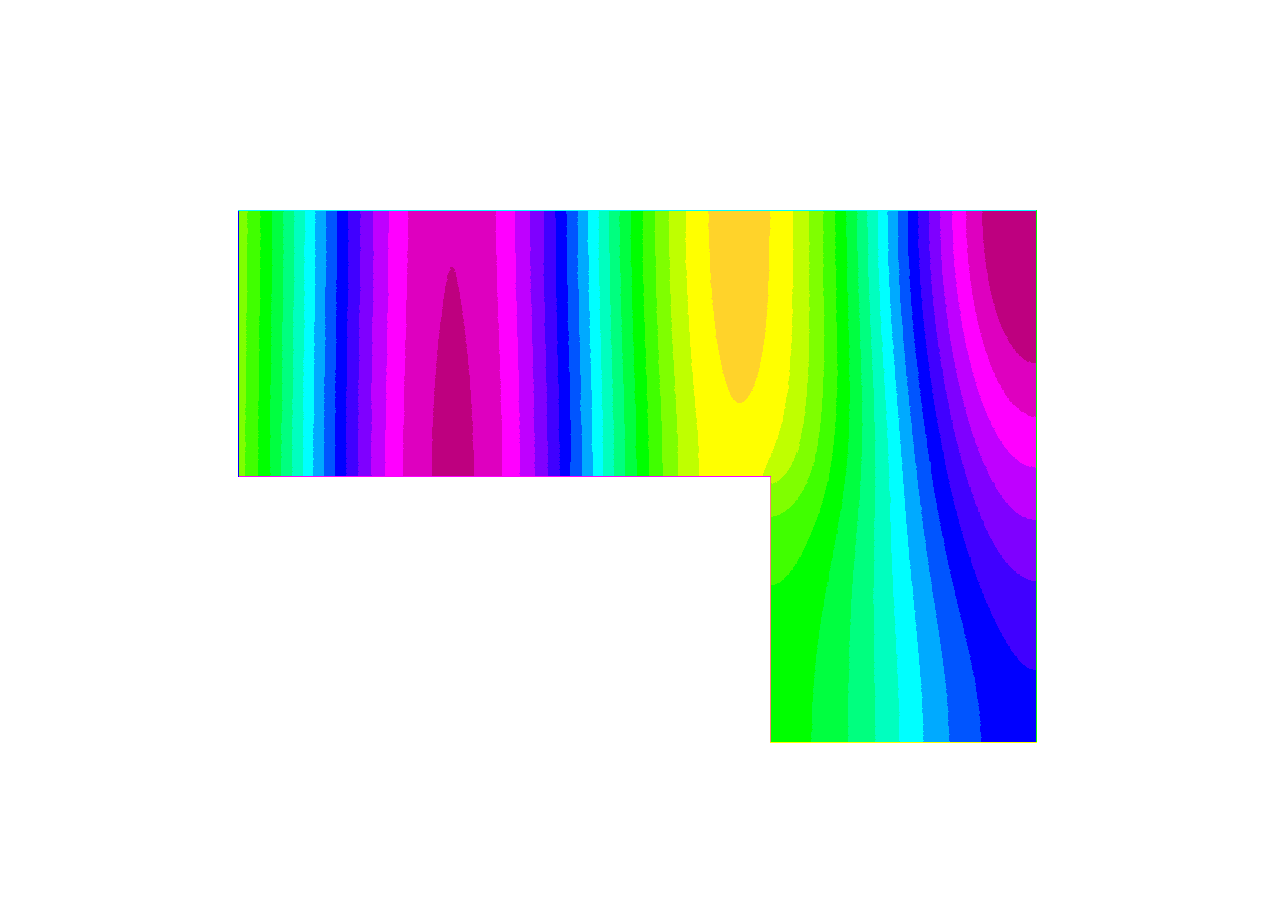
\includegraphics[width=33mm]{AcouDiff2-10.eps}
\fi
\caption{Avec condition de Neumann et pour des fréquences de~$100$, $500$ et $1000$~Hz}\label{Fig-AcouDiff2}
\end{figure}

\medskip\noindent
À quoi correspondent ces résultats?
\flushright
\textcolorgris{\reflectbox{Chaque paroi vibre à une vitesse telle que~$\rho \overline{V}_n=1$.}}
\flushleft

Sauriez-vous introduire des conditions de Robin?
\flushright
\colorgris\reflectbox{Évidemment!}\\
\reflectbox{Il suffit de changer \textrm{1i*c*k*q} en \textrm{1i*c*k*conj(q)/Z} où~$Z$ est l'impédance.}
\flushleft\colorblack

%\begin{figure}[h!]
%\centering
%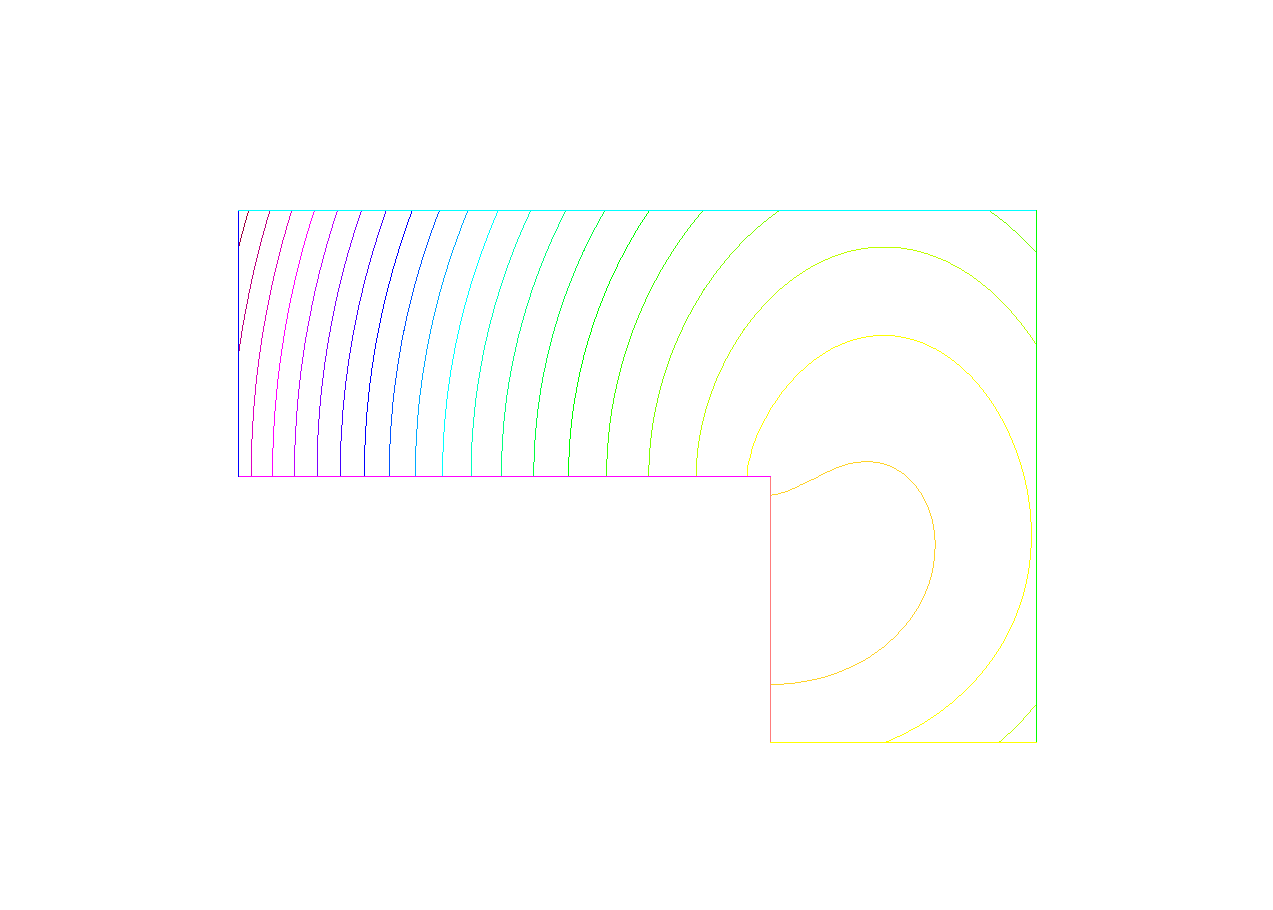
\includegraphics[width=95mm]{AcouDiff4B.eps}
%\caption{Condition aux limites de Robin}\label{Fig-AcouDiff4b}
%\end{figure}
Permettraient-elles de laisser «fuir» l'onde à l'infini?
\flushright
\colorgris\reflectbox{Oui. Pour cela il faut que l'impédance de surface soit égale à celle du milieu, i.e. ici $Z=\rho c$.}\\
\reflectbox{En terme de codage, cela correspond à \textrm{1i*k*conj(q)}.}
\flushleft\colorblack

Est-on assez loin des conditions aux limites?
\flushright
\colorgris\reflectbox{Non. Voir figure~\ref{Fig-AcouDiff4Ch}.}
\flushleft\colorblack
\begin{figure}[h!]
\centering
\ifVersionDuDocEstVincent
   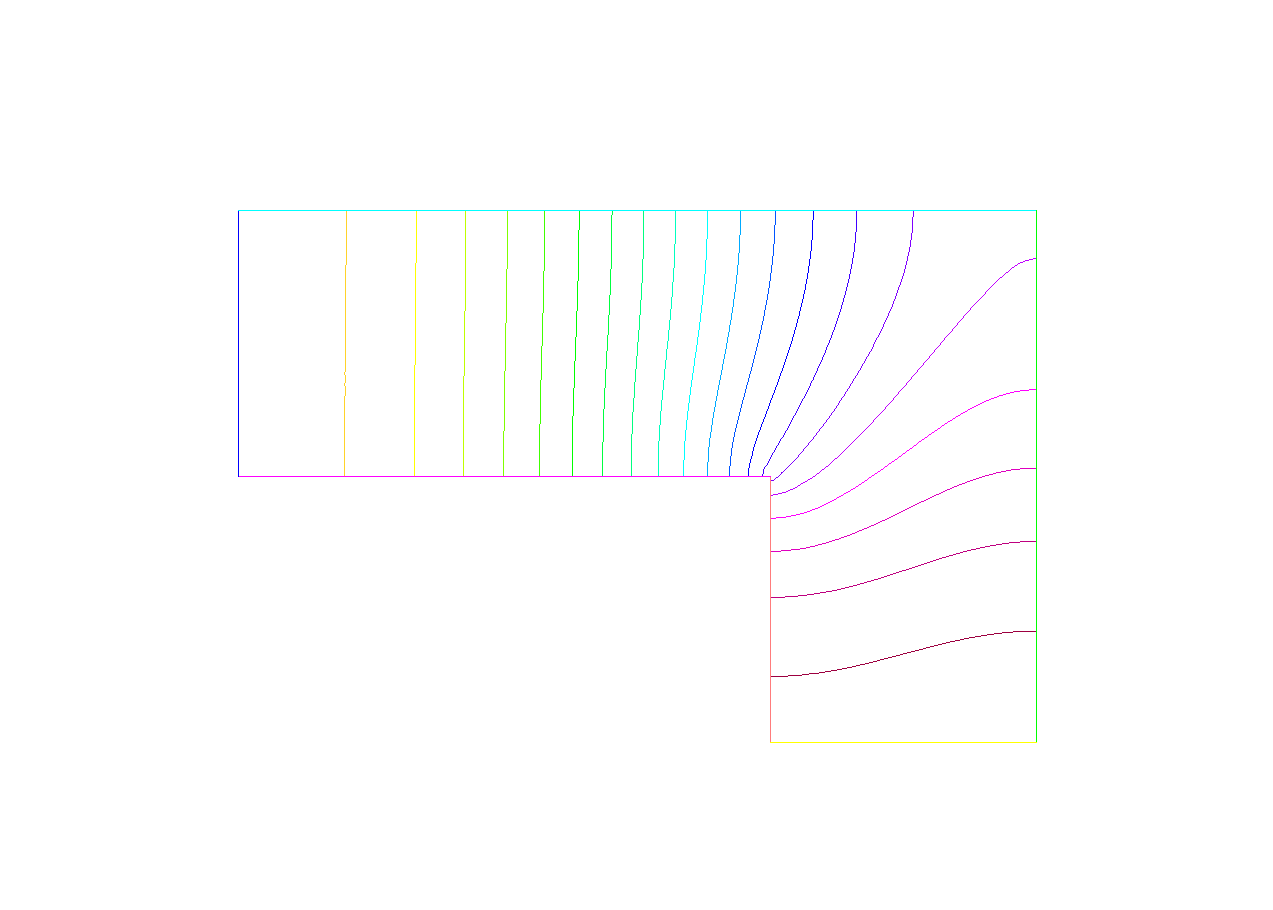
\includegraphics[width=57mm]{AcouDiff4Ch2.eps}\hfill
   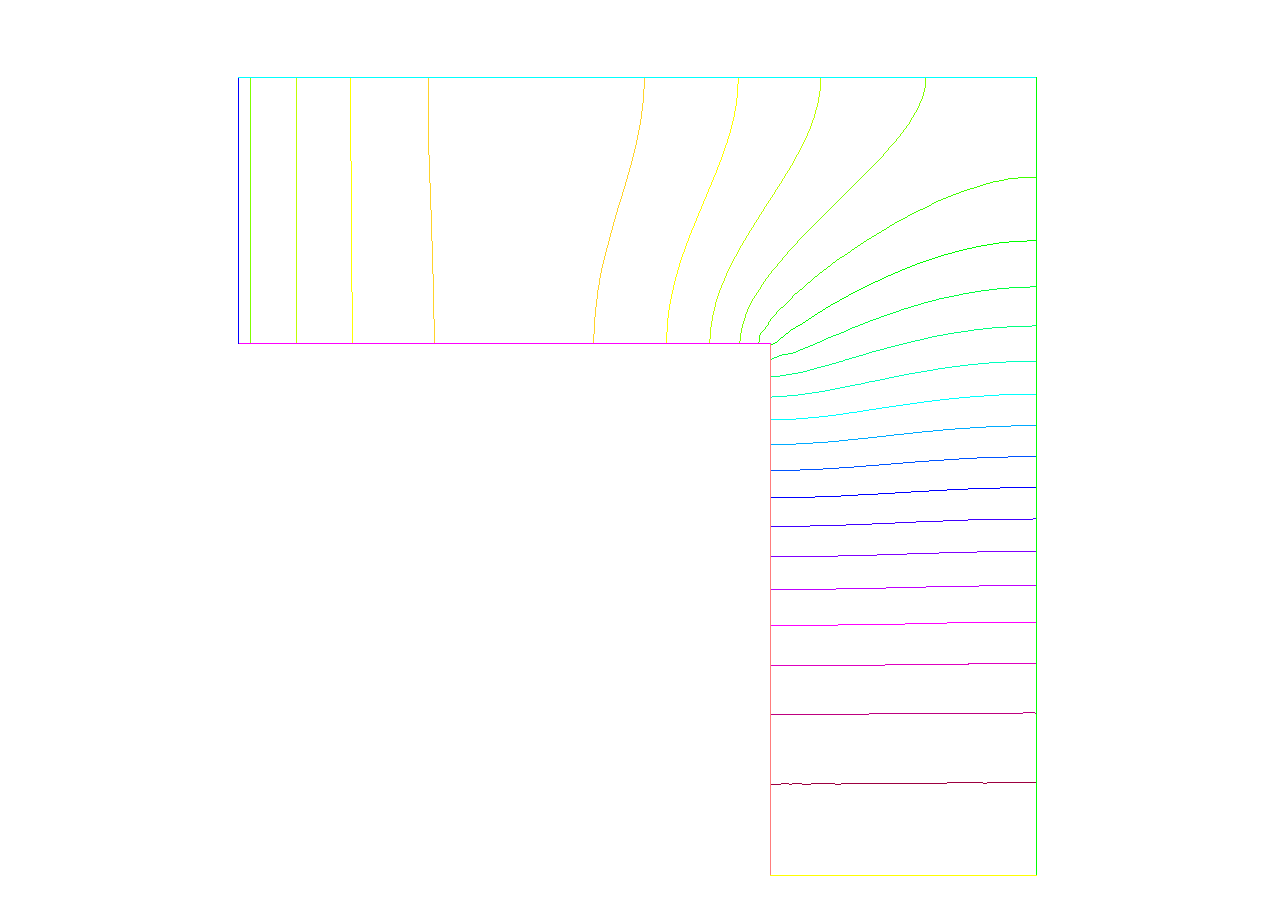
\includegraphics[width=57mm]{AcouDiff4Ch3.eps}\hfill
   \includegraphics[width=57mm]{AcouDiff4ch3l4.eps}
\else
   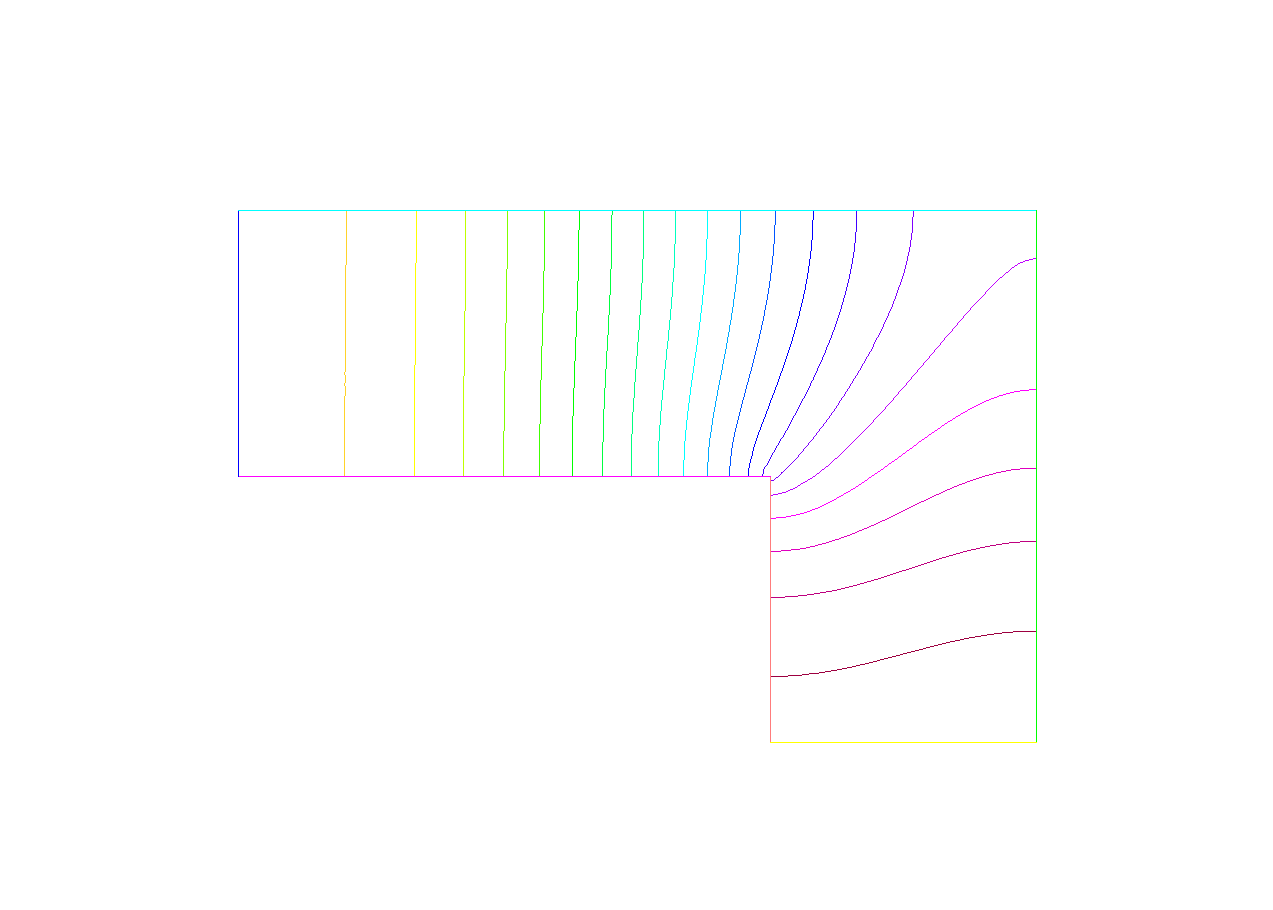
\includegraphics[width=50mm]{AcouDiff4Ch2.eps}\hfill
   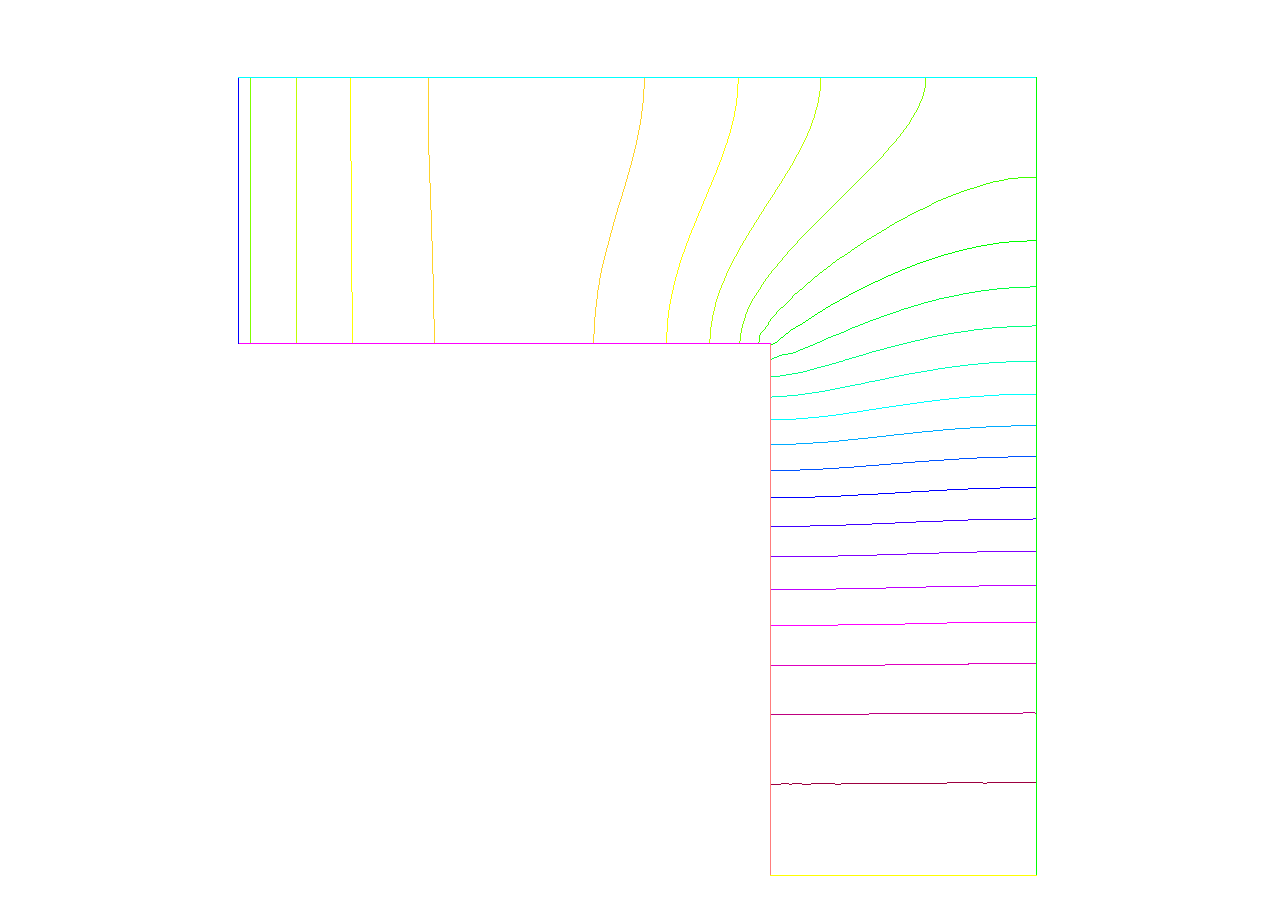
\includegraphics[width=50mm]{AcouDiff4Ch3.eps}\hfill
   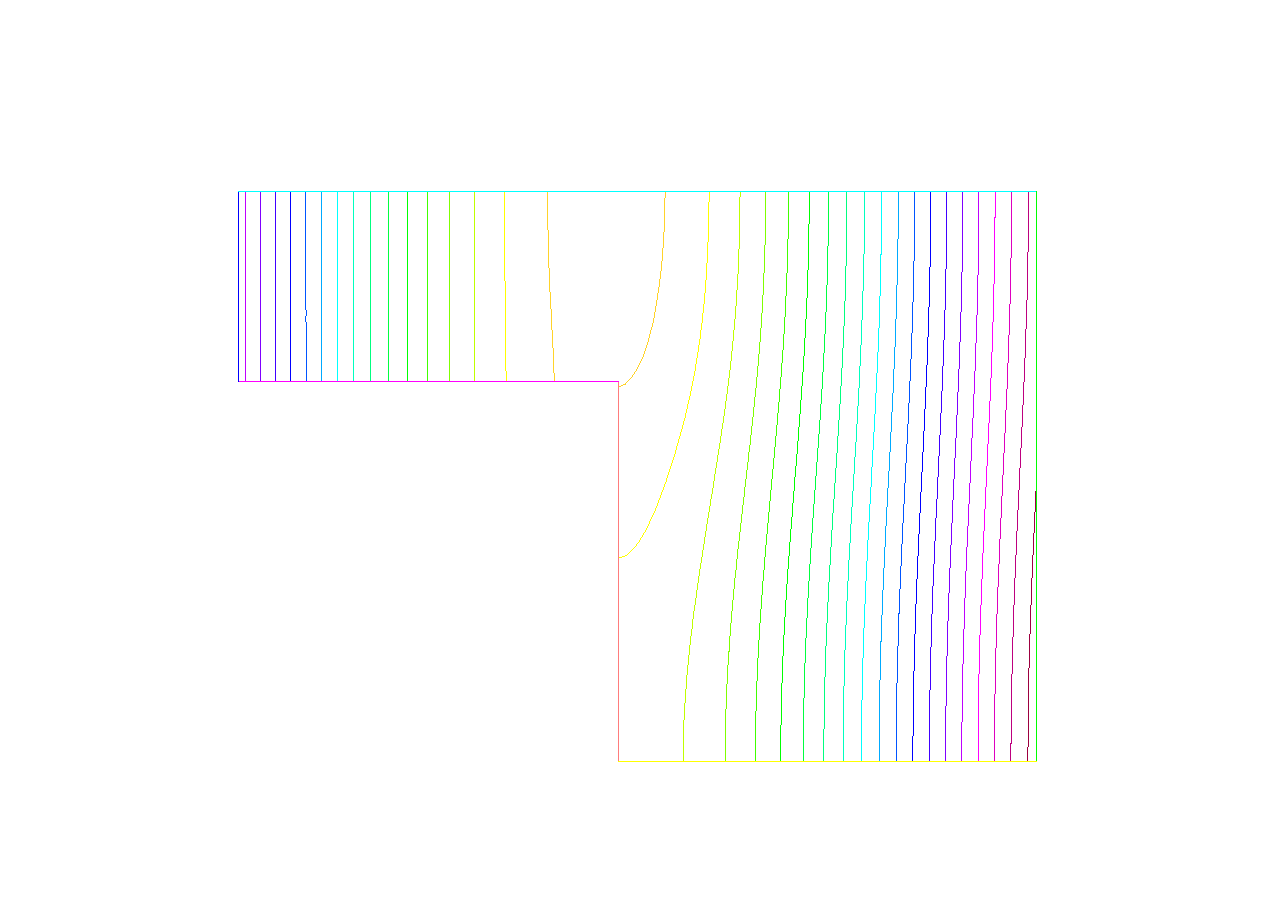
\includegraphics[width=50mm]{AcouDiff4Ch3l4.eps}
\fi
\caption{Distance aux conditions aux limtes}\label{Fig-AcouDiff4Ch}
\end{figure}


%\medskip
%\subsection{Un tablier léger}
%
%Dans les cas déjà évoqués tels qu'une source acoustique puissante faisant varier une plaque mince (tablier fin de véhicule) ou d'une vibration se propageant jusqu'à faire rayonner une surface, alors il sera effectivement nécessaire de modéliser à la fois le domaine mécanique et le domaine acoustique.
% ou un haut-parleur.

%\medskip
%\subsection{Propagation à travers plusieurs milieux}
%Pascal: air / plaque / air

%\medskip
%\subsection{Interaction fluide-structure forte: une lame dans un écoulement}
%

%\medskip
%\subsection{Ondes dans un solide}
% Comsol acou p198 : ondes dans un solide

%\medskip
%\section{Un cas qui ne fonctionne pas}
% sous réserve de trouver un cas où une excitation à la fréquence f1
% conduit à une solution à la fréquence f2:
% via un composant mécanique: on sait modéliser, donc pas d'intérêt
% via un milieu très dispersif ? à essayer
